\documentclass[11pt]{beamer}  % [t], [c], или [b] --- вертикальное выравнивание на слайдах (верх, центр, низ)
%\documentclass[handout]{beamer} % Раздаточный материал (на слайдах всё сразу)
%\documentclass[aspectratio=169]{beamer} % Соотношение сторон

%\usetheme{Berkeley} % Тема оформления
%\usetheme{Bergen}
%\usetheme{Szeged}

%\usecolortheme{beaver} % Цветовая схема
%\useinnertheme{circles}
%\useinnertheme{rectangles}

\usepackage{CS-theme/beamerthemeCS} % Подгружаем тему
%\usetheme{Warsaw} % Подгружаем тему
 
%%% Работа с русским языком
\usepackage{cmap}					% поиск в PDF
\usepackage{mathtext} 				% русские буквы в формулах
\usepackage[T2A]{fontenc}			% кодировка
\usepackage[utf8]{inputenc}			% кодировка исходного текста
\usepackage[english,russian]{babel}	% локализация и переносы

%% Beamer по-русски
\newtheorem{rtheorem}{Теорема}
\newtheorem{rproof}{Доказательство}
\newtheorem{rexample}{Пример}

%%% Дополнительная работа с математикой
\usepackage{amsmath,amsfonts,amssymb,amsthm,mathtools} % AMS
\usepackage{icomma} % "Умная" запятая: $0,2$ --- число, $0, 2$ --- перечисление
\usepackage{cancel}

%% Номера формул
%\mathtoolsset{showonlyrefs=true} % Показывать номера только у тех формул, на которые есть \eqref{} в тексте.
%\usepackage{leqno} % Нумерация формул слева

%% Свои команды
\DeclareMathOperator{\sgn}{\mathop{sgn}}

%% Перенос знаков в формулах (по Львовскому)
\newcommand*{\hm}[1]{#1\nobreak\discretionary{}
{\hbox{$\mathsurround=0pt #1$}}{}}

%%% Работа с картинками
\usepackage{graphicx}  % Для вставки рисунков
\graphicspath{{images/}{images2/}}  % папки с картинками
\setlength\fboxsep{3pt} % Отступ рамки \fbox{} от рисунка
\setlength\fboxrule{1pt} % Толщина линий рамки \fbox{}
\usepackage{wrapfig} % Обтекание рисунков текстом

%%% Работа с таблицами
\usepackage{array,tabularx,tabulary,booktabs} % Дополнительная работа с таблицами
\usepackage{longtable}  % Длинные таблицы
\usepackage{multirow} % Слияние строк в таблице

%%% Программирование
\usepackage{etoolbox} % логические операторы

%%% Другие пакеты
\usepackage{lastpage} % Узнать, сколько всего страниц в документе.
\usepackage{soul} % Модификаторы начертания
\usepackage{csquotes} % Еще инструменты для ссылок
%\usepackage[style=authoryear,maxcitenames=2,backend=biber,sorting=nty]{biblatex}
\usepackage{multicol} % Несколько колонок

%%% Картинки
\usepackage{tikz}
\usepackage{pgfplots}
\usepackage{pgfplotstable}
\usetikzlibrary{shapes,arrows}
\usetikzlibrary{arrows,positioning} 
\setlength{\parskip}{\baselineskip} 
\usetikzlibrary{arrows,decorations.text, chains,positioning,fit,calc,
  shapes.symbols,shapes.misc,shapes.geometric,
  shadows,backgrounds}
	
% Definition of circles
\def\firstcircle{(0,0) circle (1.5cm)}
\def\secondcircle{(0:2cm) circle (1.5cm)}

\colorlet{circle edge}{blue!50}
\colorlet{circle area}{blue!20}

\tikzset{filled/.style={fill=circle area, draw=circle edge, thick},
    outline/.style={draw=circle edge, thick}}	



\usepackage{stackengine}
\usepackage{multirow}
\usepackage{listings}
\lstloadlanguages{bash,c}

\lstset{escapechar=`,
	extendedchars=false,
	language=sh,
	frame=none,
	tabsize=2, 
	columns=fullflexible, 
%	basicstyle=\scriptsize,
	keywordstyle=\color{blue}, 
	commentstyle=\itshape\color{brown},
%	identifierstyle=\ttfamily, 
	stringstyle=\mdseries\color{black}, 
	showstringspaces=false, 
	numbers=left, 
	numberstyle=\tiny, 
	breaklines=true, 
	inputencoding=utf8,
	keepspaces=true,
	morekeywords={u\_short, u\_char, u\_long, in\_addr}
	}

\definecolor{darkgreen}{cmyk}{0.7, 0, 1, 0.5}

\lstdefinelanguage{diff}
{
    morekeywords={+, -},
    sensitive=false,
    morecomment=[l]{//},
    morecomment=[s]{/*}{*/},
    morecomment=[l][\color{darkgreen}]{+},
    morecomment=[l][\color{red}]{-},
    morestring=[b]",
}

\definecolor{mGreen}{rgb}{0,0.6,0}
\definecolor{mGray}{rgb}{0.5,0.5,0.5}
\definecolor{mPurple}{rgb}{0.58,0,0.82}
\definecolor{backgroundColour}{rgb}{0.95,0.95,0.92}
\usepackage{lipsum}
\usepackage{courier}

\lstdefinestyle{CStyle}{
    %backgroundcolor=\color{backgroundColour},   
    %commentstyle=\color{mGreen},
    %keywordstyle=\color{magenta},
    %numberstyle=\tiny\color{mGray},
    %stringstyle=\color{mPurple},
    %basicstyle=\footnotesize,
    %inputencoding=utf8, 
    %extendedchars=\true,
    %breakatwhitespace=false,         
    %breaklines=false,                 
    %captionpos=b,                    
    %keepspaces=false,                 
    %numbers=left,                    
    %numbersep=5pt,                  
    %showspaces=false,                
    %showstringspaces=false,
    %showtabs=false,                  
    basicstyle=\small\fontencoding{T1}\ttfamily,
  breaklines=true,
  keepspaces=true,
  extendedchars=\true,
    tabsize=2,
    language=Delphi
}
\colorlet{lightblue}{white!25!blue}
\newcommand{\WHILE}{\mbox{\sf \textcolor{lightblue}{while}}\;}
\newcommand{\DO}{\;\mbox{\sf\textcolor{lightblue}{do}}\;}
\newcommand{\AND}{\;\mbox{\sf\textcolor{lightblue}{and}}\;}
\newcommand{\OR}{\;\mbox{\sf\textcolor{lightblue}{or}}\;}
\newcommand{\WAIT}{\;\mbox{\sf\textcolor{lightblue}{wait}}\;}
\newcommand{\IF}{\;\mbox{\sf\textcolor{lightblue}{if}}\;}
\newcommand{\THEN}{\;\mbox{\sf\textcolor{lightblue}{then}}\;}
\newcommand{\ELSE}{\;\mbox{\sf\textcolor{lightblue}{else}}\;}
\newcommand{\BEGIN}{\;\mbox{\sf\textcolor{lightblue}{begin}}\;}
\newcommand{\END}{\mbox{\sf\textcolor{lightblue}{end}}\;}
\newcommand{\pair}[2]{\langle #1,\; #2 \rangle}
\newcommand{\SKIP}{\mbox{\sf\textcolor{lightblue}{skip}}\;}
\newcommand{\TRUE}{\mbox{\sf\textcolor{lightblue}{true}}\;}
\newcommand{\FALSE}{\mbox{\sf\textcolor{lightblue}{false}}\;}
\newcommand{\AWAIT}{\mbox{\sf\textcolor{lightblue}{await}}\;}
%%%%%%%%%%%%%%%%%%%%%%%%%%%%%%%%%%%%%%%%%%%%%%%%%%%%%%
\newcommand{\turn}{\mbox{\em turn}}
\newcommand{\ass}{:=}
\newcommand{\para}{\mid\mid}
\newcommand{\tab}[3]{\multicolumn{#1}{l}{}&
                     \multicolumn{#2}{l}{{#3}}}
\newcommand{\pic}{$\pi$-calculus}
\newcommand{\acquire}{\mathop{\mathit{acquire}}}
\newcommand{\release}{\mathop{\mathit{release}}}
%%%%%%%%%%%%%%%%%%%%%%%%%%%%%%%%%%%%%%%%%%%%%%%%%%%%%%
\newcommand{\assert}[1]{{\textcolor{violet}{\{#1\}}}}
\newcommand{\actif}{\mathop{\it actif}}
\newcommand{\tour}{\mathop{\it turn}}
\newcommand{\CO}{\mathit{pc}}

\usepackage{xcolor}

\definecolor{sqBlue}{RGB}{218,234,233}
\definecolor{ballBlue}{RGB}{40,156,156}

\usepackage{epstopdf}

\newcommand{\red}{}
\newcommand{\green}{}

\begin{document}
\title{Подготовительные курсы: Информатика}

\author{А.В. Якушин}
\date{\today}
\institute[ВМК МГУ им. М.В. Ломоносова]{ВМК МГУ им. М.В. Ломоносова}


 
%\includeonlylecture{lec6} % Можно поместить это в преамбулу
%\lecture{Введение}{lec0}
\subtitle{Введение в предмет}
\frame[plain]
{\titlepage}	% Титульный слайд

	\section{Описание курса}
	\begin{frame}
\frametitle{Описание курса}


\LARGE \begin{center}
Подготовка к сдаче \\Единого Государственного Экзамена\\ по информатике
\end{center}

\normalsize

\begin{block}{Преподаватели:}
Лапонина Ольга Робертовна (практика)\\
Рыбко Елена Владимировна (практика)\\
Якушин Алексей Валериевич (лекции)\\
\end{block}

\end{frame}

\begin{frame}
\frametitle{Содержание курса}


\begin{itemize}
\item Системы счисления
\item Кодирование информации
\item Алгебра логики
\item Информационные технологии
\item Алгоритмы и исполнители
\item Базовые алгоритмы
\item Подпрограммы
\item Одномерные массивы
\item Двумерные массивы
\item Теория игр
\item Олимпиадные задачи

\end{itemize}

\end{frame}


%\lecture{Лекция 1}{lec1}
\subtitle{Лекция 1 --- Системы счисления}
\frame[plain]
{\titlepage}	% Титульный слайд

	\section{Системы счисления}
	\subsection{Основные определения}
	
\begin{frame}
\frametitle{Основные определения}
\begin{block}{Система счисления}
  совокупность правил для записи (изображения, кодирования) чисел с помощью специальных символов (цифр).
\end{block}

\begin{block}{Цифра}
  специальный символ для записи чисел.
\end{block}

\begin{block}{Алфавит системы счисления}
  совокупность цифр, используемых для записи чисел.
\end{block}

\end{frame}

\begin{frame}
\frametitle{Основные определения}

\begin{block}{Позиционная система счисления}
  значение цифры зависит от ее позиции в коде числа.
\end{block}

\begin{block}{Непозиционная система счисления}
  значение цифры НЕ зависит от ее позиции в коде числа.
\end{block}

\end{frame}

\begin{frame}

\subsection{Позиционная система счисления}
\frametitle{Позиционная система счисления}

\begin{block}{Основание}
  количество различных цифр, используемых для кодирования чисел.\\
	Обозначается $p$, $p\geq 2$.
\end{block}

\begin{block}{Базис}
  последовательность степеней основания системы счисления, задающих веса разрядов.\\
	Основание $p$, веса $1,p,p^2,p^3, \ldots$
\end{block}

\end{frame}

\begin{frame}
  \frametitle{Десятичная система счисления}
	\framesubtitle{Пример}
	
\begin{itemize}
\item Рассмотрим число в десятичной системе счисления, 
$ 7086= 7\cdot 10^{3} + 0\cdot 10^{2} + 8 \cdot 10^{1}+6\cdot 10^{0} $

\item Основание $p=10$.
  
\item 10 цифр $\{0, 1, 2, \ldots ,\, 9 \}$

\end{itemize}

\end{frame}

\subsection{Формула разложения по степеням основания}
\begin{frame}
  \frametitle{Формула разложения по степеням основания}
	
\begin{block}{Целое число ($N \geq 1$)}
  $$
	a_{n}\cdot p^{n}+a_{n-1}\cdot p^{n-1}+a_{n-2}\cdot p^{n-2}+\ldots + a_{1}\cdot p+a_0=\sum_{i=0}^{n}a_i\cdot p^i
	$$
\end{block}
\begin{block}{Дробное число ($0\leq N \le 1$)}
  $$
	a_{-1}\cdot p^{-1}+a_{-2}\cdot p^{-2}+a_{-3}\cdot p^{-3}+\ldots + a_{-m}\cdot p^{-m}=\sum_{i=-1}^{-m}a_i\cdot p^i
	$$
\end{block}


\end{frame}

\begin{frame}
  \frametitle{Формула разложения по степеням основания}
	Любое число может быть представлено как в виде кода
	$$ 
	N_p=\overline{\underbrace{a_n a_{n-1} a_{n-2} \cdots  a_{1} a_{0}}_{целая\; часть}, \underbrace{a_{-1} a_{-2} \cdots  a_{-m}}_{дробная\; часть}}
	$$
так и в виде разложения по степеням основания (в виде многочлена)
  $$
	N_p=\sum_{i=0}^{n}a_i\cdot p^i + \sum_{i=-1}^{-m}a_i\cdot p^i=\sum_{i=n}^{-m}a_i\cdot p^i
	$$



\end{frame}

\begin{frame}
  \frametitle{Формула разложения по степеням основания}
	\framesubtitle{Примеры}
	$ X=123.45_{10} $
  $$	
  X_{10}=1 \cdot 10^2+2\cdot 10^1+3\cdot 10^0+4\cdot 10^{-1}+5\cdot 10^{-2}
  $$

  $ X=1101.01_2	$
	$$
  X_2 = 1\cdot 2^3 + 1\cdot 2^2 + 0\cdot 2^1 + 1\cdot 2^0 + 0\cdot 2^{-1} + 1\cdot 2^{-2} 
	$$
	
	$ X=243.36_p	$
	$$
  X_p = 1\cdot p^2 + 4\cdot p^1 + 3\cdot 2^0 + 3\cdot p^{-1} + 6\cdot p^{-2} 
	$$
	
\end{frame}

\begin{frame}
  \frametitle{Формула разложения по степеням основания}
	\framesubtitle{Несколько полезных следствий}
	\begin{itemize}
		\item $ p^k=1\underbrace{00 \ldots 00_p}_{k} $\\
		например $$2^5=100000_2$$\\
		         $$7^3=1000_7$$
		\item $ p^k-1=\underbrace{ccc\ldots\ldots cc_p}_{k} $ где $c$ наибольшая цифра\\
		например $$2^5-1=11111_2$$\\
		         $$7^3-1=666_7$$
	\end{itemize}
	
\end{frame}

\subsection{Перевод из любой системы счисления в десятичную}
\begin{frame}
  \frametitle{Перевод из любой системы счисления в десятичную}
	
	$ X=1101.01_2	$

	\begin{enumerate}
	\item Отметить разряды
	$$
	   X=\overset{\overset{3}{}}{1}\overset{\overset{2}{}}{1}\overset{\overset{1}{}}{0}\overset{\overset{0}{}}{1}.\overset{\overset{-1}{}}{0}\;\overset{\overset{-2}{}}{1}_2
	$$
	\item Разложить по степеням основания
		$$
  X_2 = 1\cdot 2^3 + 1\cdot 2^2 + 0\cdot 2^1 + 1\cdot 2^0 + 0\cdot 2^{-1} + 1\cdot 2^{-2} 
	$$
	\item Выполнить вычисления в десятичной системе счисления
	$$
  X_2 = 8+4+0+1+0+0.25=13.25_{10} 
	$$
	\end{enumerate}
  
	
	
	
	
\end{frame}

\subsection{Перевод из одной системы счисления в другую}
\begin{frame}
  \frametitle{Перевод из одной системы счисления в другую}
	\framesubtitle{Целое число}
	Пусть дано число $N$ в системе счисления с основанием $p$
	$$
	N_p=a_{n}\cdot p^{n}+a_{n-1}\cdot p^{n-1}+a_{n-2}\cdot p^{n-2}+\ldots + a_{1}\cdot p+a_0
	$$	
	Необходимо представить его в системе счисления \\ с основанием $q$
	$$
	X_q=b_{m}\cdot q^{m}+b_{m-1}\cdot q^{m-1}+b_{m-2}\cdot q^{m-2}+\ldots + b_{1}\cdot q+b_0
	$$	
	\pause
	Первую слева цифру мы не можем найти так как не знаем сколько в числе цифр
	
	\pause
	Можем найти последнюю
	
	
\end{frame}

\begin{frame}
  \frametitle{Перевод из одной системы счисления в другую}
	\framesubtitle{Целое число}
	Пусть дано число $N$ в системе счисления с основанием $p$
	$$
	N_p=a_{n}\cdot p^{n}+a_{n-1}\cdot p^{n-1}+a_{n-2}\cdot p^{n-2}+\ldots + a_{1}\cdot p+a_0
	$$	
	Необходимо представить его в системе счисления\\ с основанием $q$
	$$
	X_q=b_{m}\cdot q^{m}+b_{m-1}\cdot q^{m-1}+b_{m-2}\cdot q^{m-2}+\ldots + b_{1}\cdot q+b_0
	$$	
	\pause
	$$
	X_q=\underbrace{(b_{m}\cdot q^{m}+b_{m-1}\cdot q^{m-1}+b_{m-2}\cdot q^{m-2}+\ldots + b_{1})}_{целая\; часть \;от\; деления=N_1}\cdot q+b_0
	$$	
	\pause
	$$
	X_q=N_1\cdot q+b_0
	$$
	
	
	
\end{frame}

\begin{frame}
  \frametitle{Перевод из одной системы счисления в другую}
	\framesubtitle{Целое число: Алгоритм}
	$N_p=X_q$
	\begin{enumerate}
		\item Разделить на основание новой системы счисления
		$$ N=q\cdot N_1+b_0 $$
		\item Повторить шаг 1 с целой частью от деления
		$$ N_1=q\cdot N_2+b_1 $$
		$$ N_2=q\cdot N_3+b_2 $$
		$$ \ldots $$
		\item Закончить, когда $N_m < q $
		$X_q=b_{m}\cdot q^{m}+b_{m-1}\cdot q^{m-1}+b_{m-2}\cdot q^{m-2}+\ldots + b_{1}\cdot q+b_0$
	\end{enumerate}
	
	
\end{frame}

\begin{frame}
  \frametitle{Перевод из одной системы счисления в другую}
	\framesubtitle{Дробное число}
	Пусть дано число $N$ в системе счисления с основанием $p$
	$$
	N_p=a_{-1}\cdot p^{-1}+a_{-2}\cdot p^{-2}+a_{-3}\cdot p^{-3}+\ldots + a_{-m}\cdot p^{-m}
	$$	
	Необходимо представить его в системе счисления \\ с основанием $q$
	$$
	X_q=b_{-1}\cdot q^{-1}+b_{-2}\cdot q^{-2}+b_{-3}\cdot q^{-3}+\ldots + b_{-k}\cdot q^{-k}
	$$	
	\pause
	Последнюю слева цифру мы не можем найти так как не знаем сколько в числе цифр
	
	\pause
	Можем найти первую
	
	
\end{frame}

\begin{frame}
  \frametitle{Перевод из одной системы счисления в другую}
	\framesubtitle{Дробное число}
	Пусть дано число $N$ в системе счисления с основанием $p$
	$$
	N_p=a_{-1}\cdot p^{-1}+a_{-2}\cdot p^{-2}+a_{-3}\cdot p^{-3}+\ldots + a_{-m}\cdot p^{-m}
	$$	
	Необходимо представить его в системе счисления \\ с основанием $q$
	$$
	X_q=b_{-1}\cdot q^{-1}+b_{-2}\cdot q^{-2}+b_{-3}\cdot q^{-3}+\ldots + b_{-k}\cdot q^{-k}
	$$	
	\pause
	$$
	qX_q=b_{-1}+b_{-2}\cdot q^{-1}+b_{-3}\cdot q^{-2}+\ldots + b_{-k+1}\cdot q^{-k+1}
	$$
	
	\pause
	$qN_p=b_{-1}+N_1$
	$$
	qX_q=\underbrace{b_{-1}}_{цифра}+\underbrace{b_{-2}\cdot q^{-1}+b_{-3}\cdot q^{-2}+\ldots + b_{-k+1}\cdot q^{-k+1}}_{дробная \; часть}
	$$
	
	
\end{frame}

\begin{frame}
  \frametitle{Перевод из одной системы счисления в другую}
	\framesubtitle{Дробное число: Алгоритм}
	$N_p=X_q$
	\begin{enumerate}
		\item Умножить на основание новой системы счисления
		$$ qN=b_{-1}+N_1 $$
		\item Повторить шаг 1 с дробной частью \\
		$ qN_1=b_{-2}+N_2 $\\
		$ qN_2=b_{-3}+N_3 $\\
		$ \ldots $
		\item Закончить, когда:
		\begin{itemize}
			\item $N_i =0 $ или 
			\item дробная часть повторилась или 
			\item получено заданное количество знаков в дробной части
		\end{itemize}
		
		
	\end{enumerate}
	
	
\end{frame}


\begin{frame}
 \frametitle{Перевод из одной системы счисления в другую}
	\framesubtitle{Примеры}
	
\begin{tabular}{cccc}
Целое число 
	\pause & \begin{tabular}{c|c}
231 & 1\tabularnewline
\pause
115 & 1\tabularnewline
\pause
57 & 1\tabularnewline
\pause
28 & 0\tabularnewline
\pause
14 & 0\tabularnewline
\pause
7 & 1\tabularnewline
\pause
3 & 1\tabularnewline
\pause
1 & 1\tabularnewline
\end{tabular}
\pause & \raisebox{-0.5\height}{\includegraphics[width=0.5cm,height=4cm]{images/up.png}}
\pause
 & $231_{10}=11100111_2$\tabularnewline
\end{tabular}

	
\end{frame}


\begin{frame}
 \frametitle{Перевод из одной системы счисления в другую}
	\framesubtitle{Примеры}	

\begin{tabular}{cccc}
Дробное число 
	\pause & \begin{tabular}{c|c}
\multicolumn{1}{c}{} & 725\tabularnewline
\hline 
1 & 45\tabularnewline
\pause
0 & 9\tabularnewline
\pause
1 & 8\tabularnewline
\pause
1 & 6\tabularnewline
\pause
1 & 2\tabularnewline
\pause
0 & 4\tabularnewline
\pause
0 & 8\tabularnewline

\end{tabular}
\pause & \raisebox{-0.5\height}{\includegraphics[width=0.5cm,height=4cm]{images/down.png}}
\pause
 & $0.725_{10}=0.101(1100)_2$\tabularnewline
\end{tabular}

	
\end{frame}


\subsection{Системы счисления используемые в ЭВМ}
\begin{frame}
  \frametitle{Системы счисления используемые в ЭВМ}
	\huge
	\begin{itemize}
		\item Двоичная
		\item Восьмеричная
		\item Шестнадцатеричная
	\end{itemize}
	\normalsize
\end{frame}

\begin{frame}
  \frametitle{Системы счисления используемые в ЭВМ}
	\framesubtitle{Двоичная система счисления}
	\begin{block}{Основание}
	  $p=2$
	\end{block}
	\begin{block}{Цифры}
	  $\{0, \; 1\}$
	\end{block}
	
	\begin{block}{Пример числа}
	  $100_2$
	\end{block}
\end{frame}


\begin{frame}
  \frametitle{Системы счисления используемые в ЭВМ}
	\framesubtitle{Восьмеричная система счисления}
	\begin{block}{Основание}
	  $p=8$
	\end{block}
	\begin{block}{Цифры}
	  $\{0,1, 2, 3, 4, 5, 6, 7\}$
	\end{block}
	
	\begin{block}{Пример числа}
	  $437_8$
	\end{block}
\end{frame}


\begin{frame}
  \frametitle{Системы счисления используемые в ЭВМ}
	\framesubtitle{Шестнадцатеричная система счисления}
	\begin{block}{Основание}
	  $p=16$
	\end{block}
	\begin{block}{Цифры}
	  $\{0,1, 2, 3, 4, 5, 6, 7, 8, 9 , \underset{10}{A}, \underset{11}{B}, \underset{12}{C}, \underset{13}{D}, \underset{14}{E}, \underset{15}{F}\}$
	\end{block}
	
	\begin{block}{Пример числа}
	  $3BF_{16}$
	\end{block}
\end{frame}

\begin{frame}
  \frametitle{Системы счисления используемые в ЭВМ}
	\framesubtitle{Соответствие между двоичной, восьмеричной и шестнадцатеричной}
	
	Рассмотрим число $213_8$.
	
	Разложим по степеням основания $213_8=2\cdot8^2+1\cdot8+3$.\\ Для перевода в двоичную систему счисления следует выполнить все операции умножения и сложения в двоичной системе счисления. \\	
	$10\cdot1000000+1\cdot1000+11$
	
	Обратим внимание, что при сложении затрагиваются только три последних разряда числа, следовательно можно перевести из восьмеричной в двоичную, просто представив восьмеричные цифры в двоичном коде, дополнив их ведущими нулями до 3-х разрядов. $213_8=\underbrace{010}_{2}\underbrace{001}_{1}\underbrace{011_2}_{3}$
	
	
\end{frame}


\begin{frame}
  \frametitle{Системы счисления используемые в ЭВМ}
	\framesubtitle{Соответствие между двоичной, восьмеричной и шестнадцатеричной}
	\small
	\begin{center}
	\begin{tabular}{|c|c|c|c|c|}
\hline 
$X_{10}$ & $X_{16}$ & $X_{16}\Rightarrow X_{2}$ & $X_{8}\Rightarrow X_{2}$ & $X_{4}\Rightarrow X_{2}$\tabularnewline
\hline 
\hline 
0 & 0 & 0000 & 000 & 00\tabularnewline
\hline 
1 & 1 & 0001 & 001 & 01\tabularnewline
\hline 
2 & 2 & 0010 & 010 & 10\tabularnewline
\hline 
3 & 3 & 0011 & 011 & 11\tabularnewline
\hline 
4 & 4 & 0100 & 100 & \tabularnewline
\hline 
5 & 5 & 0101 & 101 & \tabularnewline
\hline 
6 & 6 & 0110 & 110 & \tabularnewline
\hline 
7 & 7 & 0111 & 111 & \tabularnewline
\hline 
8 & 8 & 1000 &  & \tabularnewline
\hline 
9 & 9 & 1001 &  & \tabularnewline
\hline 
10 & A & 1010 &  & \tabularnewline
\hline 
11 & B & 1011 &  & \tabularnewline
\hline 
12 & C & 1100 &  & \tabularnewline
\hline 
13 & D & 1101 &  & \tabularnewline
\hline 
14 & E & 1110 &  & \tabularnewline
\hline 
15 & F & 1111 &  & \tabularnewline
\hline 
\end{tabular}
	\end{center}
	\normalsize
\end{frame}

\begin{frame}
  \frametitle{Системы счисления используемые в ЭВМ}
	\framesubtitle{Соответствие между двоичной, восьмеричной и шестнадцатеричной}
	$$ 1101010100111_2$$
	
	$$ \underbrace{01}_{1}\underbrace{10}_{2}\underbrace{10}_{2}\underbrace{10}_{2}\underbrace{10}_{2}\underbrace{01}_{1}\underbrace{11}_{3} =1222213_4 $$
	
	$$ \underbrace{001}_{1}\underbrace{101}_{5}\underbrace{010}_{2}\underbrace{100}_{4}\underbrace{111}_{7} = 15247_8 $$
	
	$$ \underbrace{0001}_{1}\underbrace{1010}_{A}\underbrace{1010}_{A}\underbrace{0111}_{7} =1AA7_{16} $$
\end{frame}


\subsection{Двоичная система счисления}

\begin{frame}
  \frametitle{Двоичная система счисления}
	\framesubtitle{Арифметические операции}
	
	\begin{tabular}{cc}
 
Таблица сложения & Таблица умножения \tabularnewline

\begin{tabular}{|c|c|c|}
\hline 
+ & 0 & 1\tabularnewline
\hline 
0 & 0 & 1\tabularnewline
\hline 
1 & 1 & 10\tabularnewline
\hline 
\end{tabular} & %
\begin{tabular}{|c|c|c|}
\hline 
{*} & 0 & 1\tabularnewline
\hline  
0 & 0 & 0\tabularnewline
\hline 
1 & 0 & 1\tabularnewline
\hline 
\end{tabular}\tabularnewline
  &   \tabularnewline
 \begin{tabular}{cr}
\multirow{2}{*}{+} & \texttt{110111}\tabularnewline
 & \texttt{1011}\tabularnewline
\cline{2-2} 
 & \texttt{1000010}\tabularnewline
\end{tabular} & %
\begin{tabular}{cr}
\multirow{2}{*}{{*}} & \texttt{1011}\tabularnewline
 & \texttt{101}\tabularnewline
\cline{2-2} 
 & \texttt{1011}\tabularnewline
 & \texttt{0000\textcolor[rgb]{1,1,1}{0}}\tabularnewline
 & \texttt{1011\textcolor[rgb]{1,1,1}{00}}\tabularnewline
\cline{2-2} 
 & \texttt{110111}\tabularnewline
\end{tabular}\tabularnewline
\end{tabular}
	
\end{frame}

\begin{frame}
  \frametitle{Двоичная система счисления}
	\framesubtitle{Прямой, обратный и дополнительный код}
	\begin{block}{Прямой код}
	исходное двоичное число. (модуль в случае отрицательного)
	\end{block}
	\begin{block}{Обратный код}
	инвертированный прямой код (то есть единицы заменены нулями, а нули --- единицами).
	\end{block}
	
	\begin{block}{Дополнительный код}
	  обратный код, увеличенный на единицу.
	\end{block}
	
\end{frame}


\begin{frame}
  \frametitle{Двоичная система счисления}
	\framesubtitle{Представление отрицательных чисел в компьютере}
	Пусть будет $4$ бита в коде. Забираем 1 бит под знак. Получаем $3$ значащих разряда.\\
	$x=-5$\\ \pause

	\begin{tabular}{rl}
 Прямой код (П) & $0101$\tabularnewline
Обратный код (О) & $1010$\tabularnewline
Дополнительный код (Д)  & $1011$ \tabularnewline 
\end{tabular}\\  

\pause
	Для $n$ разрядов П+Д=$2^n$. $0101+1011=1\underbrace{0000}_{4}=0000$\\
	Ведущая $1$ отбрасывается (переполнение разрядности).\\  	 
	
\end{frame}

\begin{frame}
  \frametitle{Двоичная система счисления}
	\framesubtitle{Представление отрицательных чисел в компьютере}
	Рассмотрим числовую прямую. 
	\small
	\begin{tabular}{cccccccc|cccccccc}
0 & 1 & 2 & 3 & 4 & \textcolor[rgb]{1,0,0}{5} & 6 & 7 & 8 & 9 & \textcolor[rgb]{1,0,0}{10} & \textcolor[rgb]{1,0,0}{11} & 12 & 13 & 14 & 15\tabularnewline
-8 & -7 & -6 & -5 & -4 & -3 & -2 & -1 & 0 & 1 & 2 & 3 & 4 & 5 & 6 & 7\tabularnewline
 &  &  &  &  & \textcolor[rgb]{1,0,0}{П} &  &  &  &  & \textcolor[rgb]{1,0,0}{О} & \textcolor[rgb]{1,0,0}{Д} &  &  &  & \tabularnewline
\multicolumn{8}{c|}{Отрицательные} & \multicolumn{8}{c}{Положительные}\tabularnewline
\end{tabular}
	 \normalsize
	Отрицательное число $x$, таким образом хранится как $2^n-|x|$. ($-5\Rightarrow 16-5$)
	
	Для $n$ разрядов получаем:\\
	Положительные числа: $0\ldots 2^n-1$ ($n=4, [0..15]$)\\
	Отрицательные числа: $-2^{n-1}\ldots 2^{n-1}-1$ ($n=4, [-8..7]$)
	
\end{frame}

\begin{frame}
  \frametitle{Двоичная система счисления}
	\framesubtitle{Сложение и вычитание степеней}
	\pause
	Рассмотрим выражение при $n>k$ $$2^n+2^k=1\underbrace{00\ldots 0}_{n-k-1}1\underbrace{00\ldots0}_{k} $$.
	\pause
	Рассмотрим выражение при $n>k$ $$2^n-2^k=\underbrace{11\ldots 11}_{n-k}\underbrace{00\ldots0}_{k} $$.
	
	
\end{frame}

\subsection{Примеры решения задач}

\begin{frame}
  \frametitle{Примеры решения задач}
	\begin{block}{Задача}
	Перечислите через запятую в порядке возрастания все десятичные числа, не превосходящие $40$, запись которых в двоичной системе заканчивается на $011$.

	\end{block}
	\pause
	\begin{block}{Решение}
Выпишем двоичные числа, которые оканчиваются на $011$ и их десятичное представление:

\begin{tabular}{r|l}
0 & 011=3\tabularnewline
1 & 011=11\tabularnewline
10 & 011=19\tabularnewline
11 & 011=27\tabularnewline
100 & 011=35\tabularnewline
101 & 011=43\tabularnewline
\end{tabular}


	\end{block}
	
\end{frame}

\begin{frame}
  \frametitle{Примеры решения задач}
	\begin{block}{Задача}
	Укажите наибольшее четырёхзначное восьмеричное число, двоичная запись которого содержит 4 единицы. В ответе запишите только само восьмеричное число, основание системы счисления указывать не нужно.
	\end{block}
	\pause
	\begin{block}{Решение}
Если мы хотим получить наибольшее, то значащие 1 должны идти в начале числа. \\
Если восьмеричное число содержит 4 разряда, то его двоичное представление содержит от 10 до 12 разрядов.

Наибольшее: $111100000000_2=7400_8$\\ \pause
Наименьшее: $001000000111_2=1007_8$\\

	\end{block}
	
\end{frame}

\begin{frame}
  \frametitle{Примеры решения задач}
	\begin{block}{Задача}
	Решите уравнение $103_x+11_{10}=103_{x+1}$ . Ответ запишите в десятичной системе счисления. 
	\end{block}
	\pause
	\begin{block}{Решение}
Переведем все в десятичную.
$$ x^2+3+11=(x+1)^2+3$$
$$ x^2+14=x^2+2x+1+3$$
$$ 2x=10 $$
$$ x=5 $$
	\end{block}
	
\end{frame}

\begin{frame}
  \frametitle{Примеры решения задач}
	\begin{block}{Задача}
	Сколько единиц в двоичной записи числа $4^{2018} + 8^{305} – 2^{130} – 120$
	\end{block}
	\begin{block}{Решение}
	\begin{enumerate}
	\pause
	\item Переведем все к одной степени $2^{4036} + 2^{915} – 2^{130} – 2^7+2^3$
	\pause
	\item Установим чередование знаков $2^{4036} + 2^{915} +2^{130} - 2^{130}– 2^{130} – 2^7+2^3=$\\
	$=2^{4036} + 2^{915} -2^{130} - 2^{130}+2^{130} – 2^7+2^3=2^{4036} + 2^{915} -2^{131} + 2^{130} – 2^7+2^3$
	\pause
	\item Подсчет
     $\underbrace{2^{4036}}_{1} + \underbrace{2^{915} -2^{131}}_{915-131} + \underbrace{2^{130} – 2^7}_{130-7}+\underbrace{2^3}_{1}$
		\pause
		\item Ответ: 909
	\end{enumerate}
	\pause
	
	В общем случае 
	$$
	-2^n=-2^{n+1}+2^n
	$$
	
	\end{block}
	
\end{frame}
%\lecture{Лекция 2}{lec2}
\subtitle{Лекция 2 --- Информация и кодирование}
\frame[plain]
{\titlepage}	% Титульный слайд

\section{Информация и кодирование}
\section{Информация}
 \subsection{Информация}
\begin{frame}
\frametitle{Основные определения}


\begin{block}{Информация}
  Информация (от лат. informatio) — отражение реального (материального) мира, выраженное в виде сигналов и знаков.

\end{block}

\pause

\begin{block}{Информатика}
Изучает способы хранения, обработки, передачи, классификации, визуализации и т.п. информации.
\end{block}
\pause
\begin{block}{Информация и ее представление}
Различают
 \begin{itemize}
 \item{представление или изображение информации (внешняя форма);}
 \item{значение (абстрактная информация)}
 \item{отношение к реальному миру (связь абстрактной информации с действительностью)}
 \end{itemize}
 
\end{block}

\end{frame}

\begin{frame}
\frametitle{Основные определения}
\begin{block}{Информационная технология}
Конкретный способ хранения, обработки, передачи, классификации, визуализации и т.п. информации.
\end{block}
\pause
\begin{block}{Виды информационных технологий}
\begin{itemize}
	\item Обработка текста
	\item Обработка графики
	\item СУБД
	\item Обработка больших данных
	\item и др.
\end{itemize}
\end{block}

\end{frame}

\begin{frame}[fragile,squeeze]{Данные, информация, знания}

\begin{block}{Сигнал, сообщение}
 Это физический уровень информации. Например сигнал светофора или звуковые колебания.
\end{block}
\pause
\begin{block}{Данные}
 Дискретные или аналоговые сигналы, которые может обработать компьютер.
\end{block}
\pause
\begin{block}{Знания}
 Большие массивы данных объединенные сложной внутренней структурой. 
\end{block}
\end{frame}

\begin{frame}[fragile,squeeze]{Данные, информация, знания}

\begin{block}{Свойства информации}
 \begin{itemize}
	 \item абстрактность
	 \item неотделимость от носителя
 \end{itemize}
 \end{block}

\end{frame}

 \subsection{Информационный процесс}
\begin{frame}[fragile,squeeze]{Информационный процесс}


\begin{block}{Информационный процесс}
 Информационный процесс описывает посдедовательность действий, выполняемых с информацией или данными.
 Система, реализующая информационный процесс, называется информационной системой.
 \end{block}
\begin{block}{Виды информационных процессов}
 \begin{itemize}
	 \item передача информации
	 \item хранение информации
	 \item обработка информации
	 \item восприятие (распознавание) информации
 \end{itemize}
 \end{block}
\end{frame}


\section{Кодирование и измерение информации}
\subsection{Основы комбинаторики}
\begin{frame}
\frametitle{Комбинаторика}
Комбинаторика --- раздел математики, который изучает задачи выбора и расположения элементов из некоторого основного множества в соответствии с заданными правилами. 

Формулы и  принципы  комбинаторики  используются  в  теории информации для расчета количества информации, в теории вероятности, статистике и в других науках. 

Мы будем рассматривать комбинаторные формулы на множествах содержащих только не повторяющиеся элементы.
\end{frame}


\begin{frame}
\frametitle{Правила суммы и произведения}
{\bf Правило суммы.} Если элемент $a$ можно выбрать $m$ способами, а элемент
$b$ - $n$ способами, причём любой выбор элемента $a$ отличен от любого выбора
элемента $b$, то выбор <<$a$ или $b$>>$\;$ можно сделать

$m+n$ способами.

\pause

{\bf Правило произведения.} Если элемент $a$ можно выбрать $m$ способами, а элемент
$b$ - $n$ способами, то выбор пары элементов <<$a$ и $b$>>$\;$ можно сделать

 $m\cdot n$ способами.
\end{frame}

\begin{frame}
\frametitle{Правила суммы и произведения}
\framesubtitle{Примеры}
\textbf{Задача:} Монету бросают трижды. Сколько разных последовательностей орлов и решек можно при этом получить?
\pause
\textbf{Решение}

В каждом броске есть 2 варианта, соответственно получаем

$$ \underline{2}\cdot \underline{2} \cdot \underline{2} = 8 $$


\end{frame}

\begin{frame}
\frametitle{Правила суммы и произведения}
\framesubtitle{Примеры}
\textbf{Задача:} Cколько существует различных семизначных телефонных номеров (cчитается, что номер начинаться с нуля не может)? 
\pause
\textbf{Решение}

Первую цифру можно выбрать 9 способами, а каждую из шести остальных – 10 способами. Итого, $9\cdot10^6$ способов

\end{frame}

\begin{frame}
\frametitle{Перестановки}
{\bf Перестановки} Числом перестановок без повторений из $n$ элементов называется количество способов выписать в строчку все эти $n$ элементов. 

Оно обозначается $P_n$ и находится по формуле $P_n=n!$.

$$ n! = n\cdot(n-1)\cdots 1$$

\end{frame}



\begin{frame}
\frametitle{Перестановки}
\framesubtitle{Примеры}
\textbf{Задача:} Сколько существует трёхзначных чисел, в записи которых цифры 1, 2, 3 встречаются ровно по одному разу?
\pause
\textbf{Решение}

На первое место можно поставить любую из трёх цифр, на второе --- любую из двух оставшихся, а на третье --- последнюю оставшуюся цифру. Таким образом, всего получается 6 чисел.

$$3! = 6$$  чисел. 

\end{frame}

\begin{frame}
\frametitle{Перестановки}
\framesubtitle{Примеры}
\textbf{Задача:} 
а) Сколькими способами 28 учеников могут выстроиться в очередь в столовую?\\
б) Как изменится это число, если Петю Иванова и Колю Васина нельзя ставить друг за другом? 
\pause
\textbf{Решение}

a) $28!$

б) Временно уберём из очереди Колю. Оставшихся учеников можно расставить 27! способами. Колю в каждую очередь можно вставить 28 способами, но два из них – перед Петей и после него – запрещены. \\
$26\cdot27!$

\end{frame}

\begin{frame}
\frametitle{Размещения}
{\bf Размещения} Числом размещений  из $n$ элементов по $k$ называется количество способов выписать в строку $k$ различных элементов, каждый из которых выбран из данных $n$ (элементы могут повторяться, сточки отличающиеся порядком, считаются разными). Оно обозначается $A_n^k$ и находится
по формуле

$$A_n^k=\frac{n!}{(n-k)!}$$
\end{frame}



\begin{frame}
\frametitle{Размещения}
\framesubtitle{Примеры}
\textbf{Задача:} Сколько существует различных последо-вательностей из символов "A", "B", "C", "D" и "E" длиной ровно 3 символа? (При условии, что символы не могут повторяться.)

\pause
\textbf{Решение}

Необходимо определить количество размещений $n = 5$ элементов (символы <<A>>, <<B>>, <<C>>, <<D>> и <<E>>) в группах по $m = 3$ элемента (длина цепочек символов). Для этого воспользуемся формулой:

$$A_5^3=\frac{n!}{(n-k)!}=\frac{5!}{(5-3)!}=\frac{5!}{2!}=3\cdot4\cdot5=60$$

\end{frame}

\begin{frame}
\frametitle{Сочетания}
{\bf Сочетания.} Числом сочетаний из $n$ 
элементов по $k$ называется количество способов выбрать $k$ элементов из данных
$n$ различных элементов (наборы, отличающиеся лишь порядком, считаются
одинаковыми). 

Оно обозначается $C_n^k$ и находится по формуле

$$C_n^k=\frac{A_n^k}{P_k}=\frac{n!}{k!(n-k)!}$$.


\end{frame}



\begin{frame}
\frametitle{Сочетания}
\framesubtitle{Примеры}
\textbf{Задача:} Пульт управления состоит из 9 переключателей, каждый из которых может пребывать в одном из двух состояний: <<включён>> или <<выключен>>. Сколько различных режимов работы оборудования может обеспечить данный пульт, если одновременно могут быть включены только любые четыре переключателя? \\
\textbf{Решение}
Необходимо определить количество возможных сочетаний $n = 9$ элементов (общее количество выключателей) в группах по $m = 4$ элемента (выключателя). При этом порядок их включения не важен.

$$С_9^4=\frac{9!}{4!(9-4)!}=\frac{9!}{4!5!}=\frac{6\cdot 7\cdot 8\cdot 9}{2\cdot 3\cdot 4}=126$$

\end{frame}

 \subsection{Дискретный и аналоговый сигнал}

\begin{frame}[fragile,squeeze]{Дискретный и аналоговый сигнал}
\begin{block}{Аналоговый сигнал}
 сигнал, у которого каждый из представляющих параметров описывается функцией времени и непрерывным множеством возможных значений (звук, свет, электрический ток).
\end{block}
\pause
\begin{block}{Дискретный сигнал}
сигнал, который является прерывистым (в отличие от аналогового) и который изменяется во времени и принимает любое значение из списка возможных значений. Список возможных значений может быть непрерывным или квантованным. 
\end{block}
\pause
\begin{block}{Цифровой сигнал}
 сигнал, который можно представить в виде последовательности дискретных (цифровых) значений. В наше время наиболее распространены двоичные цифровые сигналы
\end{block}

\end{frame}

\begin{frame}[fragile,squeeze]{Дискретный и аналоговый сигнал}
Аналоговый сигнал
 \includegraphics[height=2cm]{images/analog.png}
\pause
Дискретный сигнал
 \includegraphics[height=2cm]{images/discrete.png}

\pause
Цифровой сигнал
  \includegraphics[height=2cm]{images/digital.png}


\end{frame}

 \subsection{Понятие кода}
\begin{frame}[fragile,squeeze]{Кодирование информации}
\begin{block}{Код}
 Система правил переводящая символы одного алфавита в символы другого алфавита.
\end{block}
\pause
\begin{block}{Кодирование и декодирование}
 Перевод сообщения из одного алфавита в другой.
 Декодирование --- обратная операция.
\end{block}
\pause
\begin{block}{Кодер и декодер}
 Устройства выполняющие кодирование и декодирование.
\end{block}

Приведите пример незакодированного сообщения
\end{frame}

 \begin{frame}[fragile,squeeze]{Подходы к измерению информации}

 \begin{itemize}
	

\item АЛФАВИТНЫЙ --- основан на подсчете числа символов в сообщении. Этот подход не связывает количество информации с содержанием сообщения, позволяет реализовать передачу, хранение и обработку информации с помощью технических устройств, не теряя при этом содержания (смысла) сообщения.
\pause
\item ВЕРОЯТНОСТНЫЙ --- Согласно Шеннону, количество информации в сообщении характеризуется уменьшением неопределенности какой-либо ситуации после получения сообщения. \\
По Шеннону, информация --- уменьшение неопределенности наших знаний.
 \end{itemize}

\end{frame}
 \subsection{Алфавитный подход}
\begin{frame}[fragile,squeeze]{Алфавит и язык}

 Для сообщений, которыми обмениваются люди, в большинстве случаев имеются соглашения относительно их формы.
О таких сообщениях мы говорим, что они передаются в языковой форме, что они составлены на некотором языке. При этом слово \alert{язык} используется в существенно более широком смысле, чем в случае связанного с ним понятия <<говорить>>. 

Мы знаем разговорный и письменный языки, язык глухонемых, построенный на жестах и мимике, печать для слепых
воспринимаемую осязанием и др.

\pause
\begin{block}{Алфавит}
 Набор знаков для изображения элементов языка. Алфавиты бывают конечные и бесконечные. Конечный алфавит является дискретным. Знаки в алфавите не повторяются.
\end{block}


\end{frame}


\begin{frame}[fragile,squeeze]
\frametitle{Алфавит и язык}
\framesubtitle{ Виды языков}

\begin{itemize}
	\item естественные \\создаются условно случайным образом на основе коммуникации между людьми);\pause
	\item искусственные;\\ создаются для специальных целей либо для определенных групп людей: язык математики, морской семафор, язык программирования и т.п.;\pause
	\item формальные\\характеризуются точными правилами построения выражений и их понимания, обеспечивая непротиворечивое, точное и компактное отображение свойств и отношений изучаемой предметной области (моделируемых объектов): язык логики, язык программирования.
\end{itemize}

\end{frame}

\begin{frame}[fragile,squeeze]
\frametitle{Единицы информации}

Количество символов (знаков) языка всегда конечно и называется \alert{Мощностью алфавита}.

Наименьшим пригодным для кодирования информации алфавитом является алфавит, состоящий из двух символов. Каждый из этих символов будет являться наименьшей единицей информации.
\pause

Чтобы осуществить кодирование, достаточно двух символов: 0 или 1  составляет 1 бит  ( bit )

BInary digiT --- (двоичный знак)
\end{frame}

\begin{frame}[fragile,squeeze]
\frametitle{Единицы информации}

1 байт  =  8 бит\\\pause
1 Кбайт  =  1024 байт  =  $2^{10}$ байт\\\pause
1 Мбайт  =  1024 Кбайт  =  $2^{20}$ байт\\\pause
1 Гбайт  =  1024 Мбайт  =  $2^{30}$ байт\\\pause
1 Тбайт  =  1024 Гбайт  =  $2^{40}$ байт\\\pause
1 Пбайт  =  1024 Тбайт  =  $2^{50}$ байт\\\pause
1 Эбайт  =  1024 Пбайт  =  $2^{60}$ байт\\\pause
1 Збайт  =  1024 Эбайт  =  $2^{70}$ байт\\\pause
1 Йбайт  =  1024 Збайт  =  $2^{80}$ байт\\

\end{frame}

\begin{frame}[fragile,squeeze]
\frametitle{Способы кодирования}

\textbf{Двоичное равномерное кодирование} --- каждый символ кодируется одинаковым количеством бит.

\pause
\textbf{Двоичное неравномерное кодирование} --- количество бит, использующихся для кодирования символов, различается.

\end{frame}

 \subsection{Равномерное кодирование}
\begin{frame}[fragile,squeeze]
\frametitle{Равномерное кодирование}

Код называется равномерным (или кодом постоянной длины), если все его кодовые слова содержат одинаковое число букв (одинаковую длину слов).

Для кодирования одного символа алфавита мощности $N$ потребуется минимальное количество бит $i$, равное наименьшему  показателю степени числа 2, при котором значение степени больше либо равно N. \\
Формула Хартли

$$i = log_2N.$$

При этом результат следует округлить до большего целого.

\end{frame}
\begin{frame}[fragile,squeeze]
\frametitle{Равномерное кодирование}
\framesubtitle{Пример}

\textbf{Задача:} Компьютерная игра состоит из 20 уровней, на каждом из которых игроку нужно отыскать 6 секретных ключей. При переходе с уровня на уровень у игрока остаются все найденные ключи. Какое минимальное количество бит потребуется для кодирования номеров секретных ключей?  \\ \pause
\textbf{Решение}
Определим количество ключей:	$20\cdot 6  =  120$

Таким образом, требуется закодировать 120 различных состояний в двоичной системе. 
$$i  = log_2120  =  7.$$

\end{frame}


 \subsection{Неравномерное кодирование}
\begin{frame}[fragile,squeeze]
\frametitle{Неравномерное кодирование}
Для однозначного декодирования неравномерного двоичного кода требуется выполнение условий Фано (Fano conditional):
\begin{itemize}
	\item Ни одно кодовое слово не является началом другого кодового слова (прямое условие)
\item Ни одно кодовое слово не является концом другого кодового слова (обратное условие)
\end{itemize}

Такие коды называются префиксными

\end{frame}
\begin{frame}[fragile,squeeze]
\frametitle{Неравномерное кодирование}
\framesubtitle{Пример}

Префиксный код легче всего представить в виде двоичного дерева, в котором  листы помечены  символами, которые объединяются для формирования сообщения. 

Кодировка символа определяется по пути вниз от корня дерева к листу, который содержит этот символ: 
бит 0 ---левая ветвь, бит 1 правая ветвь. В следующем дереве серые квадраты являются листами (внешними узлами). 

\end{frame}

\begin{frame}[fragile,squeeze]
\frametitle{Неравномерное кодирование}
\framesubtitle{Пример}

Префиксный код легче всего представить в виде двоичного дерева, в котором  листы помечены  символами, которые объединяются для формирования сообщения. 

\begin{tabular}{cc}

\raisebox{-0.5\height}{\includegraphics[height=4cm]{images/prefix.png}} \pause & %
\begin{tabular}{|c|c|}
\hline 
Символ & Код\tabularnewline
\hline 
a & 0\tabularnewline
\hline 
b & 111\tabularnewline
\hline 
c & 1011\tabularnewline
\hline 
d & 1010\tabularnewline
\hline 
r & 110\tabularnewline
\hline 
! & 100\tabularnewline
\hline 
\end{tabular}\tabularnewline

\end{tabular}

\end{frame}

 \subsection{Вероятностный подход}

 \begin{frame}[fragile,squeeze]
\frametitle{Вероятность}

Вероятность $(0 \leq р \leq 1)$ – количественная оценка возможности наступления какоголибо события.

В качестве события можно рассматривать исход некоего опыта. 
Множество всех возможных исходов некоторого опыта составляют полную группу событий. 

Сумма вероятностей всех возможных исходов равна 1. 

События, наступающие с одинаковой долей вероят-ности называются равновероятными.

Если есть N разных равновероятных событий, то вероятность наступления одного из них $p = \frac{1}{N}$

\end{frame}

\begin{frame}[fragile,squeeze]
\frametitle{Вероятностный подход}

$1$ бит несет информацию о наступлении одного из двух равновероятных событий.
Если событие может наступить с вероятностью $p$, то количество бит информации $i$ об этом событии определяется формулой Шеннона:
$$i=-log_2p $$ 
Если существует $N$ равновероятных событий, то формулу Шеннона можно записать в виде:
$$i=-log_2\frac{1}{N} $$ 


\end{frame}

\begin{frame}[fragile,squeeze]
\frametitle{Вероятностный подход}
\framesubtitle{Пример}

\textbf{Задача.} В лабораторию почерковедческой экспертизы было направлено $40$ образцов почерка. Заключение эксперта о том, что записку писал левша, содержит $3$ бита информации. Сколько записок, написанных правшами было передано эксперту? \\ \pause
\textbf{Решение.} Выразим из формулы Шеннона вероятность $p=2^{-i}$\\  \pause
Вероятность того, что записку писал левша: $p=2^{-3}=\frac{1}{8}$
Следовательно, количество записок, написанных левшами $\dfrac{40}{8} = 5$. 

Таким образом, записок, написанных правшами будет  $40 – 5 = 35$.




\end{frame}

\section{Представление информации в компьютере}
\begin{frame}[fragile,squeeze]
\frametitle{Представление информации в компьютере}


В ЭВМ применяется двоичная система счисления, т.е. все числа в компьютере представляются с помощью нулей и единиц, поэтому компьютер может обрабатывать только информацию, представленную в цифровой форме.




\end{frame}

 \subsection{Кодирование чисел}
\begin{frame}[fragile,squeeze]{Кодирование чисел}

\textbf{Ячейка памяти --- 1 байт}
\begin{table}
	\centering
		\begin{tabular}{|c|c|c|c|c|c|c|c|}\hline
		  0 & 0 & 0 & 1 & 1 & 0 & 1 & 1\\ 
		\hline
		\end{tabular}
\end{table}

\end{frame}


\begin{frame}[fragile,squeeze]{Неотрицательные целые числа}

Крайний правый бит называется \textbf{младшим} (least significant bit --- LSB).\\
Крайний левый бит называется \textbf{старшим} (most significant bit --- (MSB)).

Стандартный размер типа данных целое число (int) --- 2 байта.
\begin{enumerate}
\item{Получаем двоичное представление числа --- $319_{10}=100111111_2$}
\item{Дополняем слева нулями до 16 разрядов --- 0000000100111111 (Прямой код)}
\item{Получаем шестнадцатеричный код (HEX-сод) --- 013F.}
\end{enumerate}
\end{frame}

\begin{frame}[fragile,squeeze]{Отрицательные целые числа}

\textbf{Ячейка памяти --- 1 байт}
\begin{table}
	\centering
		\begin{tabular}{|c|c|c|c|c|c|c|c|}\hline
		  \alert{0} & 0 & 0 & 1 & 1 & 0 & 1 & 1\\ 
		\hline
		\end{tabular}
\end{table}

Крайний левый бит отвечает за знак. 0 --- положительное, 1 --- отрицательное.

Возникает проблема кодирования числа 0, т.к. получаются числа +0 и -0.
Для ее решения используют \textit{дополнительный код}.
Дополнение числа $-N$  до некоторого числа $M$ равно $N`=M-N$.
В случае двухбайтовой ячейки $M=2^{16}$


\end{frame}
\begin{frame}[fragile,squeeze]{Отрицательные целые числа}

\textbf{Дополнительный код числа}
\begin{enumerate}
\item{Получаем двоичное представление модуля числа --- $319_{10}=100111111_2$}
\item{Дополняем слева нулями до 16 разрядов --- 0000000100111111 (Прямой код)}
\item{Инвертируем каждый бит --- 1111111011000000 (Обратный код)}
\item{Прибавляем 1 --- 1111111011000001 (Дополнительный код)}
\item{Получаем шестнадцатеричный код (HEX-сод) --- FEC1.}
\end{enumerate}

\end{frame}

\subsection{Вещественные числа}

\begin{frame}[fragile,squeeze]{Вещественные числа}

Для хранения вещественных чисел в стандартном случае (float) используется 4 байта.

\begin{table}
	\centering
		\begin{tabular}{|r|ccc|ccc|}\hline
		  31 & 30 & ~ & 23 & 22 & ~ & 0\\ \hline
		  0 & 1 & $\ldots$ & 0 & 1 & $\ldots$ & 0\\  \hline
		  Знак & \multicolumn{3}{|c|}{Порядок}  & \multicolumn{3}{|c|}{Мантисса}\\
		\hline
		\end{tabular}
\end{table}

\end{frame}

\begin{frame}[fragile,squeeze]{Вещественные числа}

Получим машинное представление числа $-319.125_{10}$

\begin{enumerate}
\item{Получаем двоичное представление модуля числа --- $319.125_{10}=100111111.001_2$}
\item{Получаем нормализованное представление числа $100111111.001=0.100111111001\cdot10^{1001}$}
\item{Порядок числа $1001$. Т.к. порядок может быть положительным и отрицательным, то используют смещенный порядок. 
$
1001+1000000=1001001
$
}
\item{Мантисса числа $100111111001$}
\item{Знак числа $1$}
\item{Машинное представление $\overbrace{1}^{-}\overbrace{1001001}^{порядок}\overbrace{100111111001000000000000}^{мантисса}$}
\item{Получаем шестнадцатеричный код (HEX-сод) --- C99F9000.}
\end{enumerate}

\end{frame}

\begin{frame}[fragile,squeeze]
\frametitle{Кодирование чисел}
\framesubtitle{Количество информации}

Если для хранения целых чисел выделяется $n$ байт, то можно закодировать (хранить в памяти) 
$$ N=2^{8n}$$

чисел с учетом или без учета знака.

Например $n=2$байта, $N=2^{16}=65536бит=64Кбайта$.

\end{frame}

 \subsection{Кодирование текста}
\begin{frame}[fragile,squeeze]
\frametitle{Кодирование текста}

Для представления текстовой информации используется таблица нумерации символов или таблица кодировки символов, в которой каждому символу соответствует целое число (порядковый номер). Восемь двоичных разрядов могут закодировать 256 различных символов.

\pause
Какой вид кодирования здесь используется?

\pause
Известные кодовые таблицы для русского языка: ASCII, КОИ-8, CP1251, UTF8

\end{frame}

\begin{frame}[fragile,squeeze]
\frametitle{Кодирование текста}
\framesubtitle{Количество информации}

Информационный объем текста вычисляется по формуле:
$$ V=i\cdot N,$$
где $i$-количество бит используемое для хранения 1 символа, $N$ --- количество символов.
\end{frame}

\begin{frame}[fragile,squeeze]
\frametitle{Кодирование текста}
\framesubtitle{Пример}

\textbf{Задача.} Алфавит некоторого языка состоит из 54 символов. Оцените в байтах информационный объём сообщения длиной в 120 символов. \\\pause
\textbf{Решение.} Определим минимальное количество бит, которое  пот-ребуется для кодирования каждого символа алфавита.
Для кодирования 54 символов достаточно 6 бит.

Следовательно, информационный объем  сообщения составит  $6\cdot 120 = 720$  бит.  Или  90  байт.

\end{frame}
\subsection{Кодирование изображений}
\begin{frame}[fragile,squeeze]
\frametitle{Компьютерная графика}
Компьютерная графика в настоящее время сформировалась как наука об аппаратном и программном обеспечении для разнообразных изображений от простых чертежей до реалистичных образов естественных объектов. Компьютерная графика используется почти во всех научных и инженерных дисциплинах для наглядности и восприятия, передачи информации. 

Конечным продуктом компьютерной графики является изображение. Это изображение может использоваться в различных сферах, например, оно может быть техническим чертежом, иллюстрацией с изображением детали в руководстве по эксплуатации, простой диаграммой, архитектурным видом предполагаемой конструкции или проектным заданием, рекламной иллюстрацией или кадром из мультфильма.

\end{frame}
\begin{frame}[fragile,squeeze]
\frametitle{Кодирование цвета}


Цвет очень тесно связан с нашей жизнью и мы очень часто воспринимаем его как совершенно простую, обычную вещь. Понимание того, что на самом деле представляет цвет, из чего он состоит, как он создается --- решает многие проблемы. Понимание того, что цвет в реальной жизни, цвет на экране компьютера и цвет, создаваемый принтером это разные цвета успокаивает нервную систему.

Свет это очень сложный объект и полное понимание его внутренней природы, свойств ещё не известно науке. В компьютерной графике удобно рассматривать свет как поток электромагнитных волн. Белый свет представляет собой как бы смешение всех возможных цветов, среди которых выделяют семь основных (цвета радуги\index{цвета радуги}).
\end{frame}

\begin{frame}[fragile,squeeze]
\frametitle{Кодирование цвета}
Первым разложил белый свет на цвета радуги Исаак Ньютон (за что его чуть было не отлучили от церкви). Он пропустил луч света через стеклянную призму и получил радугу, затем пропустил полученные лучи через другую стеклянную призму и снова получил белый свет.

\begin{figure}[htbp] \begin{center}
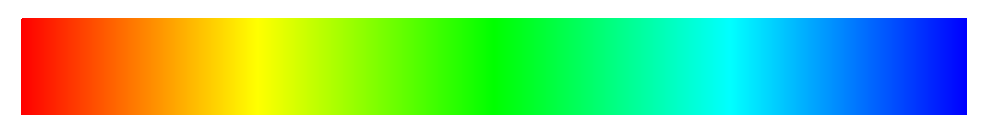
\includegraphics[width=10cm]{images/part11}

\end{center} \end{figure}
\end{frame}

\begin{frame}[fragile,squeeze]
\frametitle{Кодирование цвета}

Основные цвета в разложении белого света --- красный, оранжевый, желтый, зеленый, голубой, синий и фиолетовый образуют так называемый видимый свет видимый свет, тот свет, который воспринимается человеческм глазом. Каждый из цветов характеризуется длиной своей волны.

\end{frame}


\subsection{Цветовые модели}
\begin{frame}[fragile,squeeze]
\frametitle{Аддитивная цветовая модель RGB}
\textit{Аддитивный цвет}\index{цветовая модель!RGB} получается при соединении лучей света разных цветов. В этой системе отсутствие всех цветов представляет собой \textit{черный} цвет, а присутствие всех цветов --- \textit{белый}. Система аддитивных цветов работает с излучаемым цветом работает с излучаемым светом, например от монитора компьютера, экрана телевизора.

Эта модель используется для описания цветов, которые получаются с помощью устройств, основанных на принципе излучения. В качестве основных цветов выбран красный (Red), зеленый (Green) и синий (Blue). Иные цвета и оттенки получаются смешиванием определенного количества указанных основных цветов.
\end{frame}
\begin{frame}[fragile,squeeze]
\frametitle{Аддитивная цветовая модель RGB}

\begin{figure}[htbp] \begin{center}
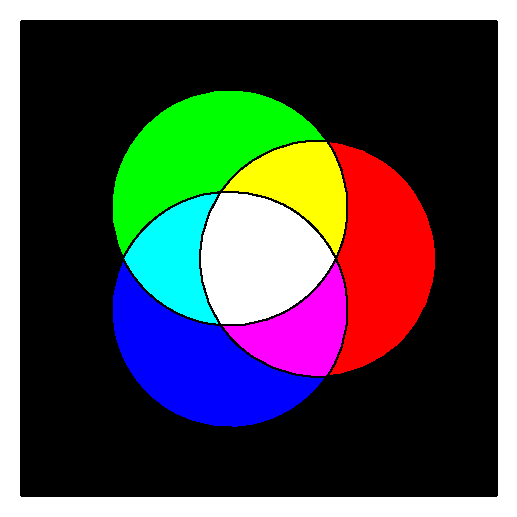
\includegraphics{images/part14}
\caption{Аддитивная модель RGB} 
\end{center} \end{figure}
\end{frame}



\begin{frame}[fragile,squeeze]
\frametitle{Субстрактивная цветовая модель CMYK}

В системе \textit{субстрактивных}\index{цветовая модель!CMYK} цветов происходит обратный процесс: цвет получается вычитанием других цветов из луча света. В этой модели белый цвет появляется в результате отсутствия всех цветов, тогда как их присутствие дает черный цвет. Система субстрактивных цветов работает с отраженным светом, например от листа бумаги. Белая бумага отражает все цвета, окрашенная - некоторые поглощает, остальные отражает.

Название данной модели CMYK составлено из названий основных субтрактивных цветов - голубого (Cyan), пурпурного (Magenta) и желтого (Yellow).
\end{frame}
\begin{frame}[fragile,squeeze]
\frametitle{Субстрактивная цветовая модель CMYK}

\begin{figure}[htbp] \begin{center}
\includegraphics{images/part16}
\end{center} \end{figure}
\end{frame}


\begin{frame}[fragile,squeeze]
\frametitle{Кодирование цвета. Палитра}

Для того чтобы компьютер имел возможность работать с цветными изображениями, необходимо представлять цвета в виде чисел - кодировать цвет. 

Способ кодирования зависит от цветовой модели и формата числовых данных в компьютере.

Для модели RGB каждая из компонент может представляться числами, ограниченными некоторым диапазоном --- например, дробными числами от 0 до 1 либо целыми числами от 0 до некоторого максимального значения. 

\end{frame}

\begin{frame}[fragile,squeeze]
\frametitle{Кодирование цвета. Палитра}

В настоящее время достаточно распространенным является формат True Color, в котором каждая компонента представлена в виде байта, что дает 256 градаций для каждой компоненты: R=0...255, G = 0...255, В = 0...255. 

Количество цветов составляет $256\times256\times256 = 16.7$ млн ($2^{24}$).
\end{frame}

\begin{frame}[fragile,squeeze]
\frametitle{Растровые изображения}

Растровая графика описывает объект цветными точками --- пикселями, определенным образом размещенными в координатной сетке.
Изображение описывается положением и цветом всех точек, из которых, как из мозаики, складывается единый объект.
Редактируя растровые объекты, можно менять только точки, а не линии.
Вся площадь изображения разбивается на некоторое число строк и столбцов. В каждой ячейке полученной матрицы находится элемент, называемый \textit{пикселом}\index{пиксель} (от англ. picture element).

\end{frame}

\begin{frame}[fragile,squeeze]
\frametitle{Растровые изображения}

Основной характеристикой такого элемента является его цвет. По существу редактирование растровых изображений сводится к изменению цветов отдельных пикселов. 

Для того, чтобы записать значение цвета в память компьютера, ему ставят в соответствие одно или несколько целых чисел, обычно, в диапазоне от 0 до 255.

Например, для черно-белой фотографии можно использовать схему, в которой черному цвету соответствует 0, белому - 255, а прочим оттенкам - целые числа внутри этого интервала 
\begin{figure}[htbp] \begin{center}
\includegraphics{images/part17}
\caption{Палитра оттенков серого}
\end{center} \end{figure}
\end{frame}



\begin{frame}[fragile,squeeze]
\frametitle{Растровые изображения}

Рассмотрим процесс преобразования рисунка в цифровую форму на примере. Возьмем черный крест на белом фоне, слева, и попробуем представить запись его компьютерного аналога.
\begin{figure}[htbp] \begin{center}
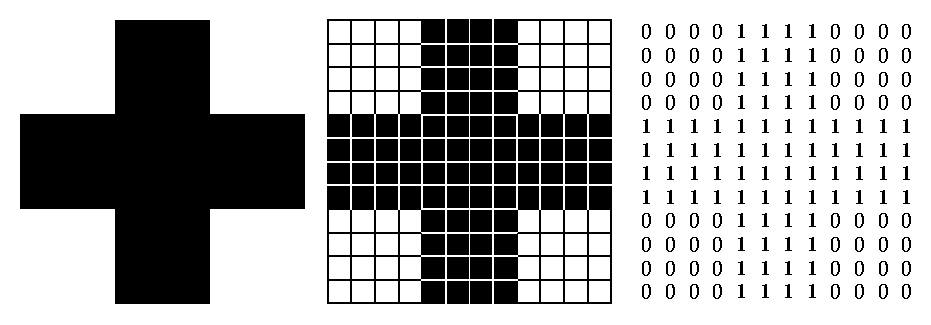
\includegraphics[height=3.5cm]{images/part18}
\end{center} \end{figure}
\end{frame} 

\begin{frame}[fragile,squeeze]
\frametitle{Растровые изображения}

\begin{figure}[htbp] \begin{center}
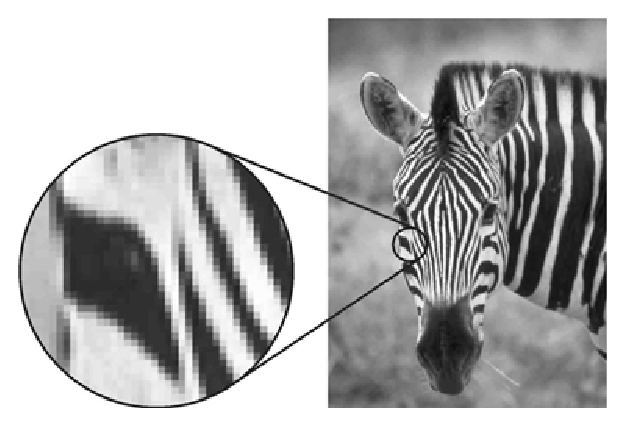
\includegraphics{images/raster}
\end{center} \end{figure}
\end{frame}

\begin{frame}[fragile,squeeze]
\frametitle{Кодирование изображений}
\framesubtitle{Количество информации}

Информационный объем растрового изображения вычисляется по формуле:
$$ V=i\cdot H\cdot W,$$
где $i$-количество бит используемое для хранения цвета 1 пиксела, $H$ --- высота изображения, $W$ --- ширина изображения.

Для хранения цвета используется алфавитный подход и равномерное кодирование.
Для вычисления количества бит, приходящихся на 1 пиксель необходимо использовать формулу Хартли.
\end{frame}

\begin{frame}[fragile,squeeze]
\frametitle{Кодирование изображений}
\framesubtitle{Пример}

\textbf{Задача.} Какой объём памяти в килобайтах необходимо выделить под хранение растрового изображения размером $256\cdot512$ пикселей, если в палитре изображения 16 цветов?
 \\ \pause
\textbf{Решение.} Определяем количество бит, необходимых для  коди-рования одного пикселя: 
$16 = 2^4$, следовательно $i=4$ бита.
Информационный объём: 
$$V=4\cdot 2^8 \cdot 2^9=2^{18} бит$$

или 64 Кбайта.

\end{frame}

 \subsection{Кодирование звука}

\begin{frame}[fragile,squeeze]
\frametitle{Аналого-цифровое преобразование}

Процесс аналого-цифрового преобразования (оцифровки) звука заключается в осуществлении замеров амплитуды сигнала с определенным временным шагом и последующей записи полученных значений в числовом виде.

Таким образом, оцифровка звука включает в себя:
\begin{itemize}
\item процесс дискретизации сигнала по времени;
\item процесс квантования по амплитуде.

\end{itemize}

\end{frame}

\begin{frame}[fragile,squeeze]
\frametitle{Аналого-цифровое преобразование}

\textbf{Частота дискретизации} (или частота семплирования, англ. Sample rate) – частота взятия отсчётов непрерывного по времени (аналогового) сигнала при его дискретизации; измеряется в кГц;

\textbf{Квантование} (англ. Quantization, bitrate, разрешение, уровень квантования, глубина дискретизации) – количество бит, необходимых для хранения одного замера (семпла). (битрейт)

В условиях задач встречается как непосредственно глубина дискретизации, так и количество уровней замеров. Тогда по количеству уровней необходимо пересчитать глубину дискретизации.


\end{frame}

\begin{frame}[fragile,squeeze]
\frametitle{Аналого-цифровое преобразование}

\includegraphics[height=7cm]{images/sound.png}

\end{frame}


\begin{frame}[fragile,squeeze]
\frametitle{Кодирование звука}
\framesubtitle{Количество информации}

Информационный объем звукового файла вычисляется по формуле:
$$ V=i\cdot k\cdot F \cdot t,$$
где $i$-количество бит используемое для хранения кванта звука (битрейт)
\\ 
$k$ --- количество канало записи,\\
$F$ --- частота\\
$t$ --- длительность в секундах\\

Для хранения звука используется алфавитный подход и равномерное кодирование.
Для вычисления количества бит, приходящихся на 1 квант звука необходимо использовать формулу Хартли.
\end{frame}

\begin{frame}[fragile,squeeze]
\frametitle{Кодирование звука}
\framesubtitle{Пример}

\textbf{Задача.} Производится одноканальная (моно) звукозапись с частотой дискретизации 48 кГц и 32-битным разрешением. Запись длится 5 минут ($5\cdot 60=300$секунд), её результаты записываются в файл, сжатие данных не производится. Определите приблизительно объем полученного файла в мегабайтах. В ответе укажите ближайшее к объему файла целое число, кратное 5.\\ \pause
\textbf{Решение.} 
$$ V=32 \cdot 1\cdot 48000\cdot 300=2^5\cdot 2^4\cdot 3 \cdot \overbrace{1000}^{8\cdot125} \cdot 3\cdot \overbrace{100}^{4\cdot 25}$$
$$ V=2^{14}\cdot 3^2 \cdot 5^5 бит!$$



\end{frame}
\begin{frame}[fragile,squeeze]
\frametitle{Кодирование звука}
\framesubtitle{Пример}


$V=2^{14}\cdot 3^2 \cdot 5^5$бит! Переведем в мегабайты
$$ V=\frac{2^{14}\cdot 3^2 \cdot 5^5}{2^{23}}=\frac{3^2 \cdot 5^5}{2^{9}}=\frac{9\cdot125 \cdot 25}{512}$$
$$ V=\frac{1125 \cdot 25}{512}=\frac{(2\cdot 512+ 101)\cdot 25}{512}=\frac{50\cdot 512+ 101\cdot 25}{512}$$
$$ V=50+\frac{101\cdot 25}{512}=50+\frac{2525}{512}=50+\frac{4\cdot 512 +477}{512}=54+\frac{477}{512}$$
Ответ 55 Мб.



\end{frame}

%\lecture{Лекция 3}{lec3}
\subtitle{Лекция 3 --- Теория множеств}

\frame[plain]
{\titlepage}	% Титульный слайд


\begin{frame}
\frametitle{Теория множеств}

\begin{center}

\Huge
Понятие множества
	
\end{center}


\end{frame}

\begin{frame}
\frametitle{Множество}

\emph{Множества} состоят из \emph{элементов}.

Запись $x\hm\in M$ означает, что $x$~является элементом множества~$M$.

Есть некоторый объект. Когда он попадает в множество, то становится его \alert{элементом}.

\begin{block}{Пример}
$$ M=\{1,2,3\}$$
\end{block}

\end{frame}
\begin{frame}
\frametitle{Множество}
Предполагается существование некоторой универсальной совокупности объектов, из которой можно хотя бы мысленно выбирать объекты, чтобы затем составлять из них множества или рассматривать, принадлежат ли они данному множеству или нет. 

На природу объектов не накладывается никаких ограничений (в частности, объекты сами могут быть
множествами), за исключением того, что объекты должны быть определенными и различными. 

\end{frame}

\begin{frame}
\frametitle{Множество}
Множество само может рассматриваться как единый объект и в качестве такового входить в состав какого-нибудь другого множества.
\end{frame}

\begin{frame}
\frametitle{Множество}
Для любых двух объектов, рассматриваемых
в качестве элементов некоторого множества, должна иметься возможность определить, различны они или нет. 

Множества определяются своими элементами --- объектами, из которых они состоят. 

Два множества равны тогда и только тогда, кода они состоят из одних и тех же элементов. 
\end{frame}

\begin{frame}
\frametitle{Виды множеств}

\begin{itemize}
	\item Конечное множество: $M=\{1,2,3\}$
	\item Бесконечное множество: $M=\{1,2,3,\ldots,n,\ldots\}$. Натуральные числа
	\item Пустое множество: не содержит элементов. Обозначается $\varnothing$
\end{itemize}
\end{frame}


\begin{frame}
\frametitle{Подмножество}

Говорят, что множество~$A$ является \emph{подмножеством}
множества~$B$ (запись: $A\hm\subset B$),
если все элементы~$A$ являются элементами~$B$.

Если $A$ подмножество~$B$, не равное всему~$B$, то~$A$~называют
\emph{собственным} подмножеством~$B$


\end{frame}

\begin{frame}
\frametitle{Количество подмножеств}

Если множество содержит $n$ элементов, то число подмножеств равно $2^n$.

Закодируем элементы, входящие в подмножество битовой цепочкой: 0 не берем элемент, 1 берем элемент.\\
Например для множества  $A=\{1,2,3,4 \}$ подмножество $B=\{2,4\}$ будет закодировано как 0101.

Соответственно количество подмножеств равно количеству чисел, которые можно закодировать с помощью $n$ бит.



\end{frame}

\begin{frame}
\frametitle{Пустое множество}

\emph{Пустое} 
множество~$\varnothing$ не содержит ни одного
элемента и является подмножеством любого множества.
\end{frame}


\begin{frame}
\frametitle{Равенство множеств}
Множества~$A$ и~$B$
\emph{равны} 
(запись: $A\hm=B$), если они
содержат одни и те же элементы (другими словами, если
$A\hm\subset B$ и~$B\hm\subset A$).

\end{frame}


\begin{frame}
\frametitle{Способы задания множеств}
\begin{enumerate}
	\item Перечислением элементов: $A=\{1,3, 100 \}$ 
	\item Описанием: Множество всех тигров России
	\item Правилом выбора элементов: $A=\{x|(x\in N)\; и\;(x \leq 5) \}$
\end{enumerate}

\end{frame}

\begin{frame}
\frametitle{Универсальное множество}

Множество, которое содержит все другие множества в качестве подмножеств называется \textbf{универсальным} множеством.

\end{frame}

\begin{frame}
\frametitle{Определить элементы множеств}

Пусть дано универсальное множество $U=\{1,2,3,4,5,6,7,8,9\}$.

\begin{enumerate}
	\item $A=\{x|x \leq 5\}$\pause
	\item $B=\{x|x\; -\; четное\}$\pause
	\item $C=\{x|3<x \leq 6\}$\pause
	\item $D=\{x|x$ делится на 3 $\}$\pause
	\item $E=\{x|x$ содержит 2 единицы в двоичном коде$\}$
\end{enumerate}

\end{frame}

\begin{frame}
\frametitle{Какие из следующих утверждений верны?}
\small
\begin{tabular}{llll}
1. $b\subset \{a,b\}$ \pause &	2. $b\in \{a,b\}$ \pause &	3. $\{b\} \subset \{a,b\}$ \pause&	4. $\{b\} \in \{a,b\}$ \pause\tabularnewline
 & & & \tabularnewline
5. $b\subset \{a,\{b\}\}$ \pause &	 6. $b\in \{a,\{b\}\}$\pause &	 7. $\{b\}\subset \{a,\{b\}\}$ \pause &	 8. $\{b\}\in \{a,\{b\}\}$\pause \tabularnewline
& & & \tabularnewline
 9. $\varnothing \in \{ \varnothing\}$ \pause& 10. $\varnothing \subset \{ \varnothing\}$ \pause & 11. $\varnothing \in \varnothing$	\pause & 12. $\varnothing \subset \varnothing$ \tabularnewline

\end{tabular}
\end{frame}

\begin{frame}
\frametitle{Сколько элементов в каждом из множеств?}

\begin{enumerate}
	\item $\{1\}$\pause
	\item $\{1,2,3\}$\pause
	\item $\{1,2,\{3\}\}$\pause
	\item $\{1,\{2,3\}\}$\pause
	\item $\{Вася\}$\pause
	\item $\{$Буквы слова <<крокодил>>$\}$
	
	
\end{enumerate}

\end{frame}

\begin{frame}
\frametitle{Сколько элементов в каждом из множеств?}

\begin{enumerate}
	\item $\{\{1\}\}$\pause
	\item $\{1,\{2\},3\}$\pause
	\item $\{\varnothing\}$\pause
	\item $\{\varnothing,\{\varnothing\}\}$\pause
	\item $\{x| x^2=-1\}$
	
	
\end{enumerate}

\end{frame}

\begin{frame}
\frametitle{Какие утверждения верны?}

Известно, что $A \subset B$ и $a \in A$.

\begin{enumerate}
	\item $a \notin B$\pause
	\item $a \in B$\pause
	\item $A\in B$\pause
	\item $a \in A \cup B $\pause
	\item $a \in A \cap B$\pause
	\item $\{a\} \subset A$\pause
	\item $\{a\} \subset B$
	
\end{enumerate}

\end{frame}


\begin{frame}
\frametitle{Теория множеств}

\begin{center}

\Huge
Операции над множествами
	
\end{center}


\end{frame}

\begin{frame}
\frametitle{Объединение}

\emph{Объединение}
$A\cup B$\index{$\cup$} состоит из элементов, которые принадлежат хотя
бы одному из множеств~$A$ и~$B$:
        $$
A \cup B = \{ x\mid x\in A \text{ или } x\in B\}.
        $$

\begin{center}
\begin{tikzpicture}
    \draw[filled] \firstcircle node {$A$}
                  \secondcircle node {$B$};
    \node[anchor=south] at (current bounding box.north) {$A \cup B$};
\end{tikzpicture}
\end{center}

\end{frame}


\begin{frame}
\frametitle{Пересечение}

\emph{Пересечение}\index{Пересечение множеств}\index{Множества!пересечение}
$A\hm\cap B$\index{$\cap$} двух множеств~$A$ и~$B$
состоит из элементов, которые принадлежат обоим множествам~$A$
и~$B$. 
        $$
A \cap B = \{ x\mid x\in A \text{ и } x\in B\}
        $$

\begin{center}
% Set A and B
\begin{tikzpicture}
    \begin{scope}
        \clip \firstcircle;
        \fill[filled] \secondcircle;
    \end{scope}
    \draw[outline] \firstcircle node {$A$};
    \draw[outline] \secondcircle node {$B$};
    \node[anchor=south] at (current bounding box.north) {$A \cap B$};
\end{tikzpicture}

\end{center}

\end{frame}


\begin{frame}
\frametitle{Разность}

\emph{Разность}
$A\setminus B$ состоит из элементов, которые принадлежат~$A$, но
не принадлежат~$B$:
        $$
A \setminus B = \{ x\mid x\in A \text{ и } x\notin B\}.
        $$

\begin{center}
% Set A and B
\begin{tikzpicture}
     \begin{scope}
        \clip \firstcircle;
        \draw[filled, even odd rule] \firstcircle node {$A$}
                                     \secondcircle;
    \end{scope}
    \draw[outline] \firstcircle
                   \secondcircle node {$B$};
    \node[anchor=south] at (current bounding box.north) {$A \setminus B$};
\end{tikzpicture}

\end{center}

\end{frame}

\begin{frame}
\frametitle{Симметрическая разность}

\emph{Симметрическая разность}\index{Множества!симметрическая разность}%
\index{Симметрическая разность множеств} $A\bigtriangleup B$%
\index{$\bigtriangleup$} состоит из
элементов, которые принадлежат ровно одному из множеств $A$
и~$B$:
        $$
A \bigtriangleup B =
 (A\setminus B)\cup (B\setminus A)=(A\cup B)\setminus (A\cap B).
        $$
				
\begin{center}
% Set A and B
\begin{tikzpicture}
      \draw[filled, even odd rule] \firstcircle node {$A$}
                                 \secondcircle node{$B$};
    \node[anchor=south] at (current bounding box.north) {$A \bigtriangleup B$};
\end{tikzpicture}

\end{center}

\end{frame}

\begin{frame}
\frametitle{Дополнение}

Если множество
$B$~является подмножеством
множества~$A$, разность $A\setminus B$
называют также \emph{дополнением~$B$ до~$A$}\index{Дополнение множества}.

 $$
\overline{A} =  \{ x\mid x\notin A\}.
        $$
				
\begin{center}
% Set A and B
\begin{tikzpicture}
      \draw [filled, even odd rule] (-4.5,4) rectangle (4.5,0);
			\draw [fill=white] (0,2) circle (1.5);
\end{tikzpicture}

\end{center}

\end{frame}

\begin{frame}
\frametitle{Диаграммы Эйлера-Венна}

 $$
(A \cap C)\cup (B \cap C)
        $$
				
\begin{center}
% Set A and B
\begin{tikzpicture}
\def\firstcircle{(90:1.0cm) circle (1.5cm)}
  \def\secondcircle{(210:1.0cm) circle (1.5cm)}
  \def\thirdcircle{(330:1.0cm) circle (1.5cm)}
      \begin{scope}
    \clip \secondcircle;
    \fill[cyan] \thirdcircle;
      \end{scope}
      \begin{scope}
    \clip \firstcircle;
    \fill[cyan] \thirdcircle;
      \end{scope}
      \draw \firstcircle node[text=black,above] {$A$};
      \draw \secondcircle node [text=black,below left] {$B$};
      \draw \thirdcircle node [text=black,below right] {$C$};
\end{tikzpicture}

\end{center}

\end{frame}


\begin{frame}
\frametitle{Теория множеств}

\begin{center}

\Huge
Основные формулы
	
\end{center}


\end{frame}

\begin{frame}
\frametitle{Дополнение}

\begin{itemize}
	\item Коммутативность $ A \cup B= B\cup A$, $ A \cap B= B\cap A$, $ A \bigtriangleup B= B \bigtriangleup A$
	\item Ассоциативность $ A \cup (B\cup C)= (A \cup B)\cup C$, $  A \cap (B\cap C)= (A \cap B)\cap C$
	\item Дистрибутивность $ A \cap (B\cup C)= (A \cap B)\cup (A \cap C)$, $ A \cup (B\cap C)= (A \cup B)\cap (A \cup C)$
\end{itemize}

\end{frame}

\begin{frame}
\frametitle{Теория множеств}


\begin{center}

\Huge
Мощность множества	
\end{center}

\end{frame}

\begin{frame}
\frametitle{Мощность множества}

Число элементов в конечном
множестве~$A$ называют также его
\emph{мощностью}
и обозначают~$|A|$ (а также~$\#A$).

\end{frame}

\begin{frame}
\frametitle{Формула включений и исключений}

\begin{align*}
    |A\cup B|        & =|A|+|B|-|A\cap B|;\\
    |A\cup B \cup C| & =|A|+|B|+|C|-\\
                     &{}-|A\cap B|-|A\cap C|-|B\cap C|+\\
                     &{}+|A\cap B\cap C|;
\end{align*}

вообще $|A_1\cup\ldots\cup A_n|$ равно
        $$
      \sum_{i}|A_i| - \sum_{i<j}|A_i \cap A_j| +
      \sum_{i<j<k} |A_i \cap A_j \cap A_k| - \ldots
        $$


\end{frame}

\begin{frame}
\frametitle{Теория множеств: Задача}
В языке запросов поискового сервера для обозначения логической операции «ИЛИ» используется символ «|», а для логической операции «И» - символ «\&». В таблице приведены запросы и количество найденных по ним страниц некоторого сегмента сети Интернет.
\begin{tabular}{|c|c|}
\hline 
 Запрос &Найдено страниц (в тысячах) \tabularnewline
\hline 
Лебедь(A) \& (Рак (B) | Щука(C)) &  320 \tabularnewline
\hline 
Лебедь \& Рак & 200 \tabularnewline
\hline 
Лебедь \& Рак \& Щука & 50 \tabularnewline
\hline 
\end{tabular}

Какое количество страниц (в тысячах) будет найдено по запросу (Лебедь \& Щука)\\
Считается, что все запросы выполнялись практически одновременно, так что набор страниц, содержащих все искомые слова, не изменялся за время выполнения запросов.

\end{frame}

\begin{frame}
\frametitle{Теория множеств: Решение}
По формуле включений и исключений имеем:
 $$
|A \cap (B \cup C)|=|A\cap C| + |A \cap B| - |A \cap B \cap C|.
$$
 
Тогда искомое количество страниц:
$$
|A \cap C| = 320 - 200 + 50 = 170
$$
\end{frame}





%\lecture{Лекция 4}{lec4}
\subtitle{Лекция 4 --- Алгебра логики. Часть 1}

\frame[plain]
{\titlepage}	% Титульный слайд


\begin{frame}
\frametitle{Алгебра логики}

\begin{center}

\Huge
Основные понятия
	
\end{center}


\end{frame}


\begin{frame}
\frametitle{Алгебра логики}

\textbf{Алгебра логики (алгебра высказываний)}~--- раздел математической
логики, в котором изучаются логические операции над высказываниями. 

\pause
Чаще
всего предполагается, что высказывания могут быть только истинными или
ложными, то есть используется так~называемая \emph{бинарная} или
\emph{двоичная} логика, в отличие от, например, троичной логики.


\end{frame}



\begin{frame}
\frametitle{Высказывания}

Высказывание в логике --- это повествовательное предложение, содержание которого может быть или истинным, или ложным.

\pause
Логические константы <<истина>> и <<ложь>> называют истинностными значениями высказывания.

\pause
Обозначения логических констант:\\
<<истина>> ---  И (Истина), T (true), 1 (единица);\\
<<ложь>> ---  Л (Ложь), F (False),  0 (ноль).


\end{frame}

\begin{frame}
\frametitle{Высказывания}

Высказывания принято обозначать заглавными буквами латинского алфавита, само содержание высказывания записывают в фигурных скобках.
\pause
\begin{block}{Пример высказывания}
 $$ A=\{ 3=2 \}$$
\end{block}
\pause
\begin{block}{Пример не высказывания}
 Сегодня идет дождь\\
 Волга впадает в Каспийское море
\end{block}

\end{frame}

\begin{frame}
\frametitle{Высказывания}

Высказывания бывают:
\begin{enumerate}
	\item простые (элементарные, атомарные);
	\item составные --- составленные комбинации из простых высказываний посредством логических связок. 
\end{enumerate}
\end{frame}


\begin{frame}
\frametitle{Логическая функция}

Логическая функция~--- это отображение вида $f: \{0, 1\}^n \rightarrow {0, 1}$, где $n$~---
число булевых переменных. В общем случае это скалярная функция векторного переменного.\pause

Логическая функция зависит от набора аргументов и принимает значения 0 или 1.\pause

Логическая функция это составное высказывание истинность компонентов которого меняется.

\end{frame}

\begin{frame}
\frametitle{Таблица истинности}

Таблица истинности --- таблица, описывающая логическую функцию. \pause

Таблица истинности --- таблица, которая показывает, какие значения примет логическая функция при всех возможных наборах значений простых выражений, входящих в него.\pause

Если имеется функция $f(x_1, x_2, \ldots, x_n)$, то вектор, представляющий эту функцию, будет единственным и иметь длину $2^n$.

\end{frame}

\begin{frame}
\frametitle{Таблица истинности}

В таблице, задающей булеву функцию от $n$ переменных, должно быть ровно $2^n$ строки~--- как раз
столько различных значений может принимать набор из $n$ переменных. \pause

Наборы значений переменных 
принято выписывать в \textit{лексикографическом порядке} (по возрастанию).

\end{frame}

\begin{frame}
\frametitle{Таблица истинности}
\framesubtitle{Правило заполнения}
В первом столбце: половина 0, половина 1, во втором половина 0, половина 1 в каждой половине и т.д.

\only<1>{
\begin{tabular}{|c|c|c|}
\hline 
x & y & z\tabularnewline
\hline 
\hline 
 &  & \tabularnewline
\hline 
 &  & \tabularnewline
\hline 
 &  & \tabularnewline
\hline 
 &  & \tabularnewline
\hline 
 &  & \tabularnewline
\hline 
 &  & \tabularnewline
\hline 
 &  & \tabularnewline
\hline 
 &  & \tabularnewline
\hline 
\end{tabular}
}
\only<2>{
\begin{tabular}{|c|c|c|}
\hline 
x & y & z\tabularnewline
\hline 
\hline 
0 &  & \tabularnewline
\hline 
0 &  & \tabularnewline
\hline 
0 &  & \tabularnewline
\hline 
0 &  & \tabularnewline
\hline 
 &  & \tabularnewline
\hline 
 &  & \tabularnewline
\hline 
 &  & \tabularnewline
\hline 
 &  & \tabularnewline
\hline 
\end{tabular}
}
\only<3>{
\begin{tabular}{|c|c|c|}
\hline 
x & y & z\tabularnewline
\hline 
\hline 
0 &  & \tabularnewline
\hline 
0 &  & \tabularnewline
\hline 
0 &  & \tabularnewline
\hline 
0 &  & \tabularnewline
\hline 
1 &  & \tabularnewline
\hline 
1 &  & \tabularnewline
\hline 
1 &  & \tabularnewline
\hline 
1 &  & \tabularnewline
\hline 
\end{tabular}
}
\only<4>{
\begin{tabular}{|c|c|c|}
\hline 
x & y & z\tabularnewline
\hline 
\hline 
0 & 0 & \tabularnewline
\hline 
0 & 0 & \tabularnewline
\hline 
0 & 1 & \tabularnewline
\hline 
0 & 1 & \tabularnewline
\hline 
1 &  & \tabularnewline
\hline 
1 &  & \tabularnewline
\hline 
1 &  & \tabularnewline
\hline 
1 &  & \tabularnewline
\hline 
\end{tabular}
}
\only<5>{
\begin{tabular}{|c|c|c|}
\hline 
x & y & z\tabularnewline
\hline 
\hline 
0 & 0 & \tabularnewline
\hline 
0 & 0 & \tabularnewline
\hline 
0 & 1 & \tabularnewline
\hline 
0 & 1 & \tabularnewline
\hline 
1 & 0 & \tabularnewline
\hline 
1 & 0 & \tabularnewline
\hline 
1 & 1 & \tabularnewline
\hline 
1 & 1 & \tabularnewline
\hline 
\end{tabular}
}
\only<6>{
\begin{tabular}{|c|c|c|}
\hline 
x & y & z\tabularnewline
\hline 
\hline 
0 & 0 & 0\tabularnewline
\hline 
0 & 0 & 1\tabularnewline
\hline 
0 & 1 & \tabularnewline
\hline 
0 & 1 & \tabularnewline
\hline 
1 & 0 & \tabularnewline
\hline 
1 & 0 & \tabularnewline
\hline 
1 & 1 & \tabularnewline
\hline 
1 & 1 & \tabularnewline
\hline 
\end{tabular}
}
\only<7>{
\begin{tabular}{|c|c|c|}
\hline 
x & y & z\tabularnewline
\hline 
\hline 
0 & 0 & 0\tabularnewline
\hline 
0 & 0 & 1\tabularnewline
\hline 
0 & 1 & 0\tabularnewline
\hline 
0 & 1 & 1\tabularnewline
\hline 
1 & 0 & 0\tabularnewline
\hline 
1 & 0 & 1\tabularnewline
\hline 
1 & 1 & 0\tabularnewline
\hline 
1 & 1 & 1\tabularnewline
\hline 
\end{tabular}
}


\end{frame}


\begin{frame}
\frametitle{Таблица истинности}

Пример для функции трех переменных: $f(x,y,z)$ (функция большинства)

\begin{tabular}{|c|c|c|c|}
\hline 
x & y & z & f(x,y,z)\tabularnewline
\hline 
0 & 0 & 0 & 0\tabularnewline
\hline 
0 & 0 & 1 & 0\tabularnewline
\hline 
0 & 1 & 0 & 0\tabularnewline
\hline 
0 & 1 & 1 & 1\tabularnewline
\hline 
1 & 0 & 0 & 0\tabularnewline
\hline 
1 & 0 & 1 & 1\tabularnewline
\hline 
1 & 1 & 0 & 1\tabularnewline
\hline 
1 & 1 & 1 & 1\tabularnewline
\hline 
\end{tabular}


\end{frame}




\begin{frame}


\frametitle{Алгебра логики}

\begin{center}

\Huge
Логические операции	
\end{center}


\end{frame}

\begin{frame}
\frametitle{Отрицание}

Отрицанием высказывания А называется новое высказывание, образованное из данного с помощью логической связки~«не~…»~(«неверно, что…»), и принимающее ложное значение, когда А истинно и наоборот.

Обозначение: $\overline{x}$ или $\neg x$

Таблица истинности

\begin{tabular}{|c|c|}
\hline 
x & $\overline{x}$\tabularnewline
\hline 
0 & 1\tabularnewline
\hline 
1 & 0\tabularnewline
\hline 
\end{tabular}

\end{frame}

\begin{frame}
\frametitle{Конъюнкция}

Конъюнкция (логиеское И) двух высказываний истинна тогда и только тогда, когда оба высказывания истинны.

Обозначение: $x\wedge y$ или $xy$, $x*y$, $x\&y$, $x\cap y$.

Таблица истинности

\begin{tabular}{|c|c|c|}
\hline
$A$ & $B$ & $A \wedge B$\\
\hline
\hline
\red{0} & \red{0} & \red{0}\\
\hline
\red{0} & \green{1} & \red{0}\\
\hline
\green{1} & \red{0} & \red{0}\\
\hline
\green{1} & \green{1} & \green{1}\\
\hline
\end{tabular}

\end{frame}

\begin{frame}
\frametitle{Дизъюнкция}

Дизъюнкиция (логиеское ИЛИ) двух высказываний истинна когда хотябы одно высказывание истинно истинны.

Обозначение: $x\vee y$ или $x+y$, $x||y$, $x\cup y$.

Таблица истинности

\begin{tabular}{|c|c|c|}
\hline
$A$ & $B$ & $A \vee B$\\
\hline
\hline
\red{0} & \red{0} & \red{0}\\
\hline
\red{0} & \green{1} & \red{1}\\
\hline
\green{1} & \red{0} & \red{1}\\
\hline
\green{1} & \green{1} & \green{1}\\
\hline
\end{tabular}

\end{frame}



\begin{frame}
\frametitle{Импликация}

Импликация (ЕСЛИ ... ТО, логический вывод) двух высказываний ложна, когда посылка истинна, а заключение ложно.

Обозначение: $x\rightarrow y$.

Таблица истинности

\begin{tabular}{|c|c|c|}
\hline
$A$ & $B$ & $A \rightarrow B$\\
\hline
\hline
\red{0} & \red{0} & \red{1}\\
\hline
\red{0} & \green{1} & \red{1}\\
\hline
\green{1} & \red{0} & \red{0}\\
\hline
\green{1} & \green{1} & \green{1}\\
\hline
\end{tabular}

\end{frame}

\begin{frame}
\frametitle{Тождество}

Тождество (эквивалентность, А тоже самое что В) двух высказываний истинна, когда оба высказывания принимают одинаковые значения истинности.

Обозначение: $x\equiv y$ или $x \sim y$.

Таблица истинности

\begin{tabular}{|c|c|c|}
\hline
$A$ & $B$ & $A \equiv B$\\
\hline
\hline
\red{0} & \red{0} & \red{1}\\
\hline
\red{0} & \green{1} & \red{0}\\
\hline
\green{1} & \red{0} & \red{0}\\
\hline
\green{1} & \green{1} & \green{1}\\
\hline
\end{tabular}

\end{frame}

\begin{frame}
\frametitle{Исключающее ИЛИ}

Исключающее ИЛИ (анти эквивалентность, А не тоже самое что В) двух высказываний истинна, когда оба высказывания принимают разные значения истинности.

Обозначение: $x \oplus y$.

Таблица истинности

\begin{tabular}{|c|c|c|}
\hline
$A$ & $B$ & $A \oplus B$\\
\hline
\hline
\red{0} & \red{0} & \red{0}\\
\hline
\red{0} & \green{1} & \red{1}\\
\hline
\green{1} & \red{0} & \red{1}\\
\hline
\green{1} & \green{1} & \green{0}\\
\hline
\end{tabular}

\end{frame}

\begin{frame}
\frametitle{Логические функции: перечисление}

Важное свойство булевых функции~--- их число конечно для заданного $n$ и равно
$2^{2^n}$. То есть, каждая функция может быть задана своей \emph{таблицей истинности} или просто
\emph{пронумерована}.  

При $n = 0$ существует только две функции-константы: 0 и 1.

Рассмотрим все функции для $n = 1$:

\begin{center}
  \begin{tabular}{|c|c|c|c|c|}
    \hline
    $x$ & $f_1$ & $f_2$ & $f_3$ & $f_4$\\ \hline
    0 & 0 & 0 & 1 & 1\\ \hline
    1 & 0 & 1 & 0 & 1\\ \hline
  \end{tabular}
\end{center}

$f_1(x) = 0, f_4(x) = 1$~--- константы, $f_2(x) = x$~--- тождественная функция, $f_3(x) =
\overline{x}$~--- отрицание.
\end{frame}

\begin{frame}
\frametitle{Логические функции: перечисление}
Рассмотрим все функции для $n = 2$: \\ \scriptsize
  \begin{tabular}{|c|c|c|c|c|c|c|c|c|c|c|c|c|c|c|c|c|c|}
    \hline
    x & y & 1 & 2 & 3 & 4 & 5 & 6 & 7 & 8 & 9 & 10 & 11 & 12 & 13 & 14 & 15 & 16\\ \hline
    0 & 0 & 0 & 0 & 0 & 0 & 0 & 0 & 0 & 0 & 1 & 1 & 1 & 1 & 1 & 1 & 1 & 1\\ \hline
    0 & 1 & 0 & 0 & 0 & 0 & 1 & 1 & 1 & 1 & 0 & 0 & 0 & 0 & 1 & 1 & 1 & 1\\ \hline
    1 & 0 & 0 & 0 & 1 & 1 & 0 & 0 & 1 & 1 & 0 & 0 & 1 & 1 & 0 & 0 & 1 & 1\\ \hline
    1 & 1 & 0 & 1 & 0 & 1 & 0 & 1 & 0 & 1 & 0 & 1 & 0 & 1 & 0 & 1 & 0 & 1\\ \hline
  \end{tabular}
\normalsize
$f_1(x, y) = 0, f_{16}(x, y) = 1$~--- константы, \\ \pause
$f_2(x, y) =x~\wedge~y$, $f_{15}(x, y) =\overline{x~\wedge~y}$(штрих Шеффера)  \\\pause
$f_8(x, y) = x~\vee~y$, $f_9(x, y) = \overline{x~\vee~y}$(стрелка Пирса)\\\pause
$f_7(x, y) = x~\oplus~y$, $f_{10}(x, y) = x~\equiv~y$\\\pause
$f_{14}(x, y) =x~\rightarrow~y$,$f_{3}(x, y) =\overline{x~\rightarrow~y}$  \\ \pause
$f_{12}(x, y) =y~\rightarrow~x$,$f_{5}(x, y) =\overline{y~\rightarrow~x}$  \\ \pause

Таким образом, каждая булева функция может быть представлена как в виде таблицы истинности,
так и в виде формулы. 

\end{frame}

\begin{frame}
\frametitle{Catch phrase логических операций}


\begin{center}
\begin{tabular}{|c|c|}
\hline 
Операция & Catch phrase \tabularnewline
\hline 
\hline 
$\overline{\textcolor[rgb]{1,1,1}{x}}$ & НЕ A \pause \tabularnewline 
\hline 
$\wedge$ & A И B \pause \tabularnewline 
\hline 
$\vee$ & A ИЛИ B  \pause \tabularnewline 
\hline 
$\oplus$ & ИЛИ A ИЛИ В \pause \tabularnewline 
\hline 
$\rightarrow$ & ЕСЛИ А ТО B, А ВЛЕЧЕТ В  \pause \tabularnewline
\hline 
$\equiv$ & А ТОГДА И ТОЛЬКО ТОГДА КОГДА B \tabularnewline  
\hline 
\end{tabular}\end{center}
\end{frame}

\begin{frame}
\frametitle{Приоритет логических операций}

Сначала выполняется операция с самым низким приоритетом.
\begin{center}
\begin{tabular}{|c|c|c|}
\hline 
Приоритет & Операция & Описание\tabularnewline
\hline 
0 & $\overline{x}$ & Отрицание \tabularnewline
\hline 
1 & $\wedge$ & Конъюнкция\tabularnewline
\hline 
2 & $\vee,\oplus$ & Дизъюнкция, Исключающее ИЛИ\tabularnewline
\hline 
3 & $\rightarrow$ & Импликация \tabularnewline
\hline 
4 & $\equiv$ & Тождество\tabularnewline
\hline 
\end{tabular}
\end{center}
\end{frame}

\begin{frame}
\frametitle{Приоритет логических операций}
\framesubtitle{Пример}

\only<1>{$$ \overline{x} \rightarrow (x \vee \overline{y} \wedge z) $$}
\only<2>{ $$ \underbrace{\overline{x}}_{1} \rightarrow (x \vee \underbrace{\overline{y}}_{2} \wedge z) $$}
\only<3>{ $$ \underbrace{\overline{x}}_{1} \rightarrow (x \vee \underbrace{\underbrace{\overline{y}}_{2} \wedge z}_{3}) $$}
\only<4>{ $$ \underbrace{\overline{x}}_{1} \rightarrow (\underbrace{x \vee \underbrace{\underbrace{\overline{y}}_{2} \wedge z}_{3}}_{4}) $$}
\only<5>{ $$ \underbrace{\underbrace{\overline{x}}_{1} \rightarrow (\underbrace{x \vee \underbrace{\underbrace{\overline{y}}_{2} \wedge z}_{3}}_{4})}_{5} $$}

\end{frame}



\begin{frame}[fragile,squeeze]{Таблица истинности}
Рассмотрим формулу $F(x_1,x_2,x_3) = {\bar x}_1 \wedge (x_2\oplus x_3)$ 
Составим таблицу истинности~--- сначала выпишем столбец ${\bar x}_1$, затем столбец $(x_2\oplus x_3)$,
а затем конъюнкцию этих двух столбцов.

\medskip
\begin{tabular}{|c|c|c||c|c|c|}
  \hline
  $x_1$ & $x_2$ & $x_3$ & $\bar x_1$ & $x_2\oplus x_3$ & $F$ \\
  \hline
   0  &  0  & 0         & 1          &  0              & 0 \\
   0  &  0  & 1         & 1          &  1              & 1 \\
   0  &  1  & 0         & 1          &  1              & 1 \\
   0  &  1  & 1         & 1          &  0              & 0 \\
   1  &  0  & 0         & 0          &  0              & 0 \\
   1  &  0  & 1         & 0          &  1              & 0 \\
   1  &  1  & 0         & 0          &  1              & 0 \\
   1  &  1  & 1         & 0          &  0              & 0 \\
  \hline
\end{tabular}
\end{frame}

\begin{frame}
\frametitle{Алгебра логики}
\begin{center}

\Huge
Законы (формулы) алгебры логики
\end{center}


\end{frame}

\begin{frame}
\frametitle{Основные законы алгебры логики}
Закон двойного отрицания: $ \overline{\overline{x}}=x $  \pause

Коммутативность:\\
 $ A \vee B = B \vee A$\\
 $ A \wedge B = B \wedge A$\\ \pause

Ассоциативность:\\
 $ A \vee (B \vee C) = (A \vee B) \vee C$\\
 $ A \wedge (B \wedge C) = (A \wedge B) \wedge C$\\ \pause

Дистибутивность:\\
$ A \wedge (B \vee C) = (A \wedge B) \vee (A\wedge C)$\\ 
$ A \vee (B \wedge C) = (A \vee B) \wedge (A \vee C)$\\
 

\end{frame}

\begin{frame}
\frametitle{Основные законы алгебры логики}
Законы де Моргана:
$$ \overline{A \vee B} = \overline{A} \wedge \overline{B} $$
$$ \overline{A \wedge B} = \overline{A} \vee \overline{B} $$ \pause

Поглощение:
$$ A \vee A\wedge B =A$$ \pause

Склейка
$$ x_1\wedge x_2 \wedge x_3 \vee x_1\wedge \overline{x_2} \wedge x_3 = x_1 \wedge x_3$$

\end{frame}

\begin{frame}
\frametitle{Примитивные формулы}
Конъюнкция:\\
$ x \wedge x$ =\pause $x$ (идемпотентность)\\
$ x \wedge \overline{x}$ =\pause $0$\\
$ x \wedge 1$ =\pause $x$\\
$ x \wedge 0$ =\pause $0$

Дизъюнкция:\\
$ x \vee x$ =\pause $x$\\
$ x \vee \overline{x}$ =\pause $1$ (закон исключения третьего)\\
$ x \vee 1$ =\pause $1$\\
$ x \vee 0$ =\pause $x$



\end{frame}

\begin{frame}
\frametitle{Примитивные формулы}
Тождество:\\
$ x \equiv x$ =\pause $1$ \\
$ x \equiv \overline{x}$ =\pause $0$\\
$ x \equiv 1$ =\pause $x$\\
$ x \equiv 0$ =\pause $\overline{x}$

Исключающее ИЛИ:\\
$ x \oplus x$ =\pause $0$\\
$ x \oplus \overline{x}$ =\pause $1$\\
$ x \oplus 1$ =\pause $\overline{x}$\\
$ x \oplus 0$ =\pause $x$



\end{frame}

\begin{frame}
\frametitle{Примитивные формулы}
Импликация:\\
$ x \rightarrow x$ =\pause $1$ \\
$ x \rightarrow \overline{x}$ =\pause $\overline{x}$\\
$ \overline{x} \rightarrow x $ =\pause $x$\\
$ x \rightarrow 1$ =\pause $1$\\
$ 1 \rightarrow x$ =\pause $x$\\
$ x \rightarrow 0$ =\pause $\overline{x}$
$ 0 \rightarrow x$ =\pause $1$

\end{frame}

\begin{frame}
\frametitle{Представление формул в стандартном базисе}
Набор операций: $\overline{\textcolor[rgb]{1,1,1}{x}}, \wedge, \vee$ составляет базис. \pause
 
Через базис можно выразить любые логические функции.

Например:\\
$x \rightarrow y = \overline{x} \vee y$\\ \pause
$x \oplus y = \overline{x}\wedge y \vee x\wedge \overline{y}$\\ \pause
$x \equiv y = \overline{x}\wedge \overline{y} \vee x\wedge y$\\ \pause



\end{frame}
%\lecture{Лекция 5}{lec5}
\subtitle{Лекция 5 --- Алгебра логики. Часть 2}

\frame[plain]
{\titlepage}	% Титульный слайд


\begin{frame}
\frametitle{Алгебра логики}

\begin{center}

\Huge
Построение функции по таблице истинности
	
\end{center}


\end{frame}

\begin{frame}
\frametitle{Определения}

Для начала условимся называть конъюнкцию нескольких различных переменных или их отрицаний 
\textit{элементарым конъюнктом}. 

Например $x_1\wedge x_2\wedge \bar{x}_3\wedge x_4$. 


\end{frame}

\begin{frame}
\frametitle{Функция большинства}

Функцию большинства (\textit{голосования}) $Г(x_1,x_2,x_3)$, принимающую значение равное значению наибольшего количества аргументов, можно задать следующей таблицей:

\medskip
\begin{tabular}{|c|c|c||c|}
  \hline
  $x$  & $y$ & $z$ & $Г(x,y,z)$ \\
  \hline
   0   & 0 & 0 &  0   \\
   0   & 0 & 1 &  0   \\
   0   & 1 & 0 &  0   \\
   0   & 1 & 1 &  1 \\
   1   & 0 & 0 &  0   \\
   1   & 0 & 1 &  1 \\
   1   & 1 & 0 &  1 \\
   1   & 1 & 1 &  1 \\
  \hline
\end{tabular}

\end{frame}

\begin{frame}
\frametitle{Алгоритм построения СДНФ}

1. Выберем из таблицы все строки, в которых значение функции равно 1. 

\medskip
\begin{tabular}{|c|c|c||c|l}
  \hline
  $x$  & $y$ & $z$ & $Г(x,y,z)$ & \\
  \hline
   0   & 0 & 0 &  0 &  \\
   0   & 0 & 1 &  0 &  \\
   0   & 1 & 0 &  0 &  \\
   0   & 1 & 1 &  1 & $\leftarrow$ \\
   1   & 0 & 0 &  0 &  \\
   1   & 0 & 1 &  1 & $\leftarrow$ \\
   1   & 1 & 0 &  1 & $\leftarrow$\\
   1   & 1 & 1 &  1 & $\leftarrow$\\
  \hline
\end{tabular}

\end{frame}

\begin{frame}
\frametitle{Алгоритм построения СДНФ}

2. Каждой такой строке сопоставим элементарный конъюнкт по следующему правилу: если значение переменной $p_i$ в данной строке равно 1, то в конъюнкт входит сама переменная $p_i$, иначе её отрицание $\bar{p}_i$.

\medskip
\begin{tabular}{|c|c|c||c|l}
  \hline
  $x$  & $y$ & $z$ & $Г(x,y,z)$ & \\
  \hline
   0   & 0 & 0 &  0 &  \\
   0   & 0 & 1 &  0 &  \\
   0   & 1 & 0 &  0 &  \\
   0   & 1 & 1 &  1 & $\bar{x}\wedge y \wedge z $ \\
   1   & 0 & 0 &  0 &  \\
   1   & 0 & 1 &  1 & $x\wedge \bar{y} \wedge z$ \\
   1   & 1 & 0 &  1 & $x\wedge y \wedge \bar{z}$\\
   1   & 1 & 1 &  1 & $x\wedge y \wedge z$\\
  \hline
\end{tabular}


\end{frame}

\begin{frame}
\frametitle{Алгоритм построения СДНФ}

3. Далее все четыре конъюнкта соединяются при помощи
дизъюнкции:
$$
F(x,y,z) = (\bar x\wedge y\wedge z)\vee(x \wedge \bar y \wedge z)\vee(x \wedge y \wedge \bar z)\vee(x \wedge y \wedge z).
$$

\begin{tabular}{|c|c|c||c|l}
  \hline
  $x$  & $y$ & $z$ & $Г(x,y,z)$ & \\
  \hline
   0   & 0 & 0 &  0 &  \\
   0   & 0 & 1 &  0 &  \\
   0   & 1 & 0 &  0 &  \\
   0   & 1 & 1 &  1 & $\bar{x}\wedge y \wedge z $ \\
   1   & 0 & 0 &  0 &  \\
   1   & 0 & 1 &  1 & $x\wedge \bar{y} \wedge z$ \\
   1   & 1 & 0 &  1 & $x\wedge y \wedge \bar{z}$\\
   1   & 1 & 1 &  1 & $x\wedge y \wedge z$\\
  \hline
\end{tabular}

\end{frame}

\begin{frame}
\frametitle{Алгоритм построения СДНФ}

Полученная форумла называется \textit{совершенной дизъюнктивной нормальной формой} (сокращенно СДНФ) функции голосования.
Оказывается, что $F(x,y,z)$ реализует как раз функцию голосования.
$$
F(x,y,z) = (\bar x\wedge y\wedge z)\vee(x \wedge \bar y \wedge z)\vee(x \wedge y \wedge \bar z)\vee(x \wedge y \wedge z).
$$

\end{frame}

\begin{frame}
\frametitle{Алгоритм построения СДНФ}

4. Упрощение. Используем основные правила

Поглощение:
$$ A \vee A\wedge B =A$$ \pause

Склейка
$$ x_1\wedge x_2 \wedge x_3 \vee x_1\wedge \overline{x_2} \wedge x_3 = x_1 \wedge x_3$$

Сравниваем каждый конъюнкт к каждым. Если возможно применить формулу, то упрощаем, если нет, то оставляем конъюнкт в исходной форме.

\end{frame}

\begin{frame}
\frametitle{Алгоритм построения СДНФ}

\only<1>{$$
F(x,y,z) = (\bar x\wedge y\wedge z)\vee\underbrace{(x \wedge \bar y \wedge z)}_{нет}\vee\underbrace{(x \wedge y \wedge \bar z)}_{нет}\vee\underbrace{(x \wedge y \wedge z)}_{да}.
$$}

\only<2>{$$
F(x,y,z) = \underbrace{(\bar x\wedge y\wedge z)}_{нет}\vee(x \wedge \bar y \wedge z)\vee\underbrace{(x \wedge y \wedge \bar z)}_{нет}\vee\underbrace{(x \wedge y \wedge z)}_{да}.
$$}
\only<3>{$$
F(x,y,z) = \underbrace{(\bar x\wedge y\wedge z)}_{нет}\vee\underbrace{(x \wedge \bar y \wedge z)}_{нет}\vee(x \wedge y \wedge \bar z)\vee\underbrace{(x \wedge y \wedge z)}_{да}.
$$}

\only<1>{$$
F(x,y,z) = (y\wedge z)
$$}
\only<2>{$$
F(x,y,z) = (y\wedge z)\vee (x\wedge z)
$$}
\only<3>{$$
F(x,y,z) = (y\wedge z)\vee (x\wedge z)\vee ( x\wedge y)
$$}



\end{frame}


\begin{frame}
\frametitle{Алгебра логики}

\begin{center}

\Huge
Логические элементы	
\end{center}


\end{frame}

\begin{frame}
\frametitle{Логические элементы	}

Логический элемент в электронных схемах – это устройство, реализующее ту или
иную логическую функцию. При этом логические сигналы 0 и 1 задаются разными
уровнями напряжения.

Для изображения логических схем всегда используются условные графические
обозначения элементов, описывающие только выполняемую элементами функцию и не
зависящие от его схемы. В настоящее время в мире существует несколько общепринятых
стандартов условных обозначений. 



\end{frame}

\begin{frame}
\frametitle{Логические элементы	}

Наиболее распространенными являются
американский стандарт milspec 806В и стандарт МЭК 117-15 А, созданный
Международной Электротехнической Комиссией. 

Часто в литературе используются
также обозначения в европейской системе DIN 4070. 

В отечественной литературе
условные обозначения элементов в основном соответствуют ГОСТ 2.743-82.


\end{frame}

\begin{frame}
\frametitle{Логические элементы	}

\begin{figure}[htbp] \begin{center}
\includegraphics[height=5cm]{images/logic}

\end{center} \end{figure}


\end{frame}
\begin{frame}
\frametitle{Cхема для функции голосования	}$
F(x,y,z) = (y\wedge z)\vee (x\wedge z)\vee ( x\wedge y)$\\
\begin{figure} \begin{center}
\includegraphics[height=7cm]{images/vote}

\end{center} \end{figure}


\end{frame}

\begin{frame}
\frametitle{Алгебра логики}

\begin{center}

\Huge
Как вычисления выполняются автоматически?

\end{center}

\end{frame}

\begin{frame}{Двоичные сумматоры}
\begin{itemize}
	\item \alert{Полусумматор} (HA) складывает два бита и получает бит \alert{сумма} и бит \alert{перенос} разряда.
	\item \alert{Сумматор} (FA) складывает два бита с учетом переноса разряда от предыдущего действия и получает бит \alert{сумма} и бит  \alert{перенос} разряда для следующего сложения. (разобрать самостоятельно)
\end{itemize}
\end{frame}


\begin{frame}{Полусумматор}
\begin{center}
\begin{tabular}{|c|c|c|c|}
	\hline
	\multicolumn{2}{|c|}{Вход} & \multicolumn{2}{c|}{Выход} \\
	\hline
	$x$ & $y$ & Сумма (s) & Перенос  (w) \\
	\hline\hline
	0   & 0   & 0   & 0     \\
	0   & 1   & 1   & 0     \\
	1   & 0   & 1   & 0     \\
	1   & 1   & 0   & 1     \\
	\hline
\end{tabular}
\end{center}
\pause
\begin{itemize}
	\item $s = x \oplus y=\overline{x}\wedge y \vee x\wedge \overline{y}$
	\item $w = x \wedge y$
\end{itemize}
\end{frame}

\begin{frame}{Полусумматор:схема}

\begin{itemize}
	\item $s = x \oplus y=\overline{x}\wedge y \vee x\wedge \overline{y}$
	\item $w = x \wedge y$
\end{itemize}

\includegraphics[height=5cm]{images/hs}
\end{frame}
%\lecture{Лекция 6}{lec6}
\subtitle{Лекция 6 --- Алгебра логики. Часть 3 --- Примеры решения задач}

\frame[plain]
{\titlepage}	% Титульный слайд


\begin{frame}
\frametitle{Алгебра логики}

\begin{center}

\Huge
Задача 18 ЕГЭ
	
\end{center}


\end{frame}

\begin{frame}
\frametitle{Схема решения задачи 18}

Общая схема решения задач типа задачи 18 ЕГЭ: <<Найти число А для логического выражения>>
\begin{enumerate}
	\item Замена переменных для упрощения работы с выражением
	\item Приведение выражения к стандартному виду. Если требуется тождественная истинность, то дизъюнкция выражений, если тождественная ложность, то конъюнкция выражений.
	\item Определение <<проблемной ситуации>>: когда значение логического выражения зависит от А
	\item Формулирование условий и ограничений для числа А
	\item Поиск числа А
\end{enumerate}


\end{frame}

\begin{frame}[t]
\frametitle{Примеры задача 18}
\framesubtitle{Задачи с отрезками}

На числовой прямой даны отрезки $A = [70; 90]$, $B = [40; 60]$ и $C = [0; N]$ и функция \\
$F(x) = (\overline{(x \in A)} \rightarrow (x \in B) ) \wedge (\overline{(x \in C)} \rightarrow (x \in A) )$
При каком наименьшем числе $N$ функция $F(x)$ истинна более чем для $30$ целых чисел $x$?


	\only<1>{1. Введем обозначение $A=A(x)=x \in A$. Для В и С аналогично. 
	
	Получим $F(x) = (\overline{A} \rightarrow B ) \wedge (\overline{С} \rightarrow A )$}
	\only<2>{2. Преобразуем: 
	 $$F(x) = \underbrace{(\overline{A} \rightarrow B )}_{A \vee B} \wedge \underbrace{(\overline{С} \rightarrow A )}_{C \vee A}=(A \vee B) \wedge (C \vee A)$$
	 $$F(x) = \underbrace{(A\wedge C) \vee \underbrace{(A\wedge A)}_{A}}_{Поглощение A} \vee (B \wedge C) \vee \underbrace{(B\wedge A)}_{Поглощение A}=A \vee (B\wedge C)
	$$}
	
\end{frame}

\begin{frame}[t]
\frametitle{Примеры задача 18}
\framesubtitle{Задачи с отрезками}

	
	3. нарисуем отрезки на числовой оси:\\
	\includegraphics[height=2cm]{images/t18_1}
	\pause
	Составим таблицу для всех частей числовой прямой.
	\begin{tabular}{|c|c|c|c|c|}
\hline 
Интервал & A & B & C & F\tabularnewline
\hline 
$(-\infty;0]$ & 0 & 0 &  & 0\tabularnewline
\hline 
$[0;40]$ & 0 & 0 &  & 0\tabularnewline
\hline 
$[40;60]$ & 0 & 1 &  & \tabularnewline
\hline 
$[60;70]$ & 0 & 0 &  & 0\tabularnewline
\hline 
$[70;90]$ & 1 & 0 &  & 1\tabularnewline
\hline 
$[90;+\infty)$ & 0 & 0 &  & 0\tabularnewline
\hline 
\end{tabular}

	
	


\end{frame}

\begin{frame}[t]
\frametitle{Примеры задача 18}
\framesubtitle{Задачи с отрезками}

	
	Определим <<ПРОБЛЕМУ>>: когда нужен отрезок $C$?
	\begin{tabular}{|c|c|c|c|c|}
\hline 
Интервал & A & B & C & F\tabularnewline
\hline 
$(-\infty;0]$ & 0 & 0 & не влияет & 0\tabularnewline
\hline 
$[0;40]$ & 0 & 0 & не влияет & 0\tabularnewline
\hline 
$[40;60]$ & 0 & 1 & \textbf{ПРОБЛЕМА} & \tabularnewline
\hline 
$[60;70]$ & 0 & 0 & не влияет & 0\tabularnewline
\hline 
$[70;90]$ & 1 & 0 & не влияет & 1\tabularnewline
\hline 
$[90;+\infty)$ & 0 & 0 & не влияет & 0\tabularnewline
\hline 
\end{tabular}

	\pause
	
	4. Получается, что всегда есть $90-70+1=21$ число для которого выражение истинно.\\
	Нам нужно набрать более 30 чисел. Значит число $N$ должно попасть в отрезок $[40;60]$
	
	\pause 
	5. Следовательно:  $10=N-40+1 \Rightarrow N=49$
	


\end{frame}

\begin{frame}[t]
\frametitle{Примеры задача 18}
\framesubtitle{Задачи с серией условий}

Для какого наибольшего целого числа А формула
$$( (x \leq 9) \rightarrow (x\cdot x \leq A) ) \wedge ( (y\cdot y \leq A) \rightarrow (y \leq 9) )$$
тождественно истинна (то есть принимает значение 1 при любых целых неотрицательных значениях переменных x и y)?
	\begin{enumerate}
		\item Замена не требуется 	\pause 
		\item Преобразование не требуется 	\pause 
		\item Когда возникает <<ПРОБЛЕМА>>?  	\pause 
		$$( \underbrace{(x \leq 9)}_{1} \rightarrow (x\cdot x \leq A) ) \wedge ( (y\cdot y \leq A) \rightarrow \underbrace{(y \leq 9)}_{0} )$$ В этом случае все зависит от А.
		
		
	\end{enumerate}
	
	
	
\end{frame}

\begin{frame}[t]
\frametitle{Примеры задача 18}
\framesubtitle{Задачи с серией условий}

Для какого наибольшего целого числа А формула
$$( (x \leq 9) \rightarrow (x\cdot x \leq A) ) \wedge ( (y\cdot y \leq A) \rightarrow (y \leq 9) )$$
тождественно истинна (то есть принимает значение 1 при любых целых неотрицательных значениях переменных x и y)?
	\begin{enumerate}
		\setcounter{enumi}{3}
		\item $x \leq 9=1 \Rightarrow x=\{9,8,7, \ldots\}$\\ 	\pause 
		      значит $(x^2 \leq A)=1 \Rightarrow A=\{81,82,83, \ldots\}$\\ 	\pause 
		      $y \leq 9=0 \Rightarrow y>9 \Rightarrow y=\{10,11,12,\ldots\}$\\  	\pause 
					значит $(y^2 \leq A)=0 \Rightarrow y^2>A \Rightarrow A=\{99,98,97, \ldots\}$\\ 	\pause 
					следовательно $81\leq A \leq 99$ 	\pause 
	 \item наименьшее $A=81$, наибольшее $A=99$.
		
	\end{enumerate}
	
	
	
\end{frame}

\begin{frame}[t]
\frametitle{Примеры задача 18}
\framesubtitle{Задачи с серией условий}

Укажите наименьшее целое значение А, при котором выражение
$$(y + 2x < A) \vee (3y + 2x > 120) \vee (3y - x > 30)$$
истинно для любых целых положительных значений x и y.

	\begin{enumerate}
		\item Замена не требуется 	\pause 
		\item Преобразование не требуется 	\pause 
		\item Когда возникает <<ПРОБЛЕМА>>? 	\pause 
		$$(y + 2x < A) \vee \underbrace{(3y + 2x > 120)}_{0} \vee \underbrace{(3y - x > 30)}_{0}$$
		В этом случае все зависит от А.
		
		
	\end{enumerate}
	
	
\end{frame}

\begin{frame}[t]
\frametitle{Примеры задача 18}
\framesubtitle{Задачи с серией условий}
\begin{enumerate}
		\setcounter{enumi}{3}
		\item $(3y + 2x > 120)=0 \Rightarrow 3y + 2x \leq 120 (1)$\\  	\pause 
		      $(3y - x > 30)=0 \Rightarrow 3y - x \leq 30 (2)$\\ 
					умножим второе неравенство на 2 и сложим с первым \\
					$3y+2x+6y-2x \leq 120+60$\\
					$9y \leq 180 \Rightarrow 0 < y \leq 20 $\\
					В этом случае должно быть $(y + 2x < A)=1, y < A-2x (3)$\\ 	\pause 
					Следовательно нам нужно найти наибольшее возможное x и выбрать $A$ так чтобы $A-2x$ было положительным неравенство (3) выполнялось для всех $y$\\ 	\pause 
					Из (1) Наибольший $x$ соответствует наименьшему возможному $y=1$\\
					$3+2x\leq 120 \Rightarrow x \leq 58 \Rightarrow \underbrace{1+2\cdot 58}_{117} < A \Rightarrow A \geq 118$\\ 	\pause 
	 \item наименьшее $A=118$.
		
	\end{enumerate}
	
	
	
\end{frame}

\begin{frame}[t]
\frametitle{Примеры задача 18}
\framesubtitle{Задачи с поразрядными операциями}

Применение логической операции <<поразрядно>> к числам $x$ и $y$ $x R y$, $R=\{\vee, \wedge, \rightarrow, \oplus, \equiv \}$:
\begin{enumerate}
	\item Перевести оба числа в двоичную систему счисления 	\pause 
	\item Применить операцию $R$ к каждой паре разрядов. (считаем, что слева от первого значащаего разряда стоят нули, например $1010=0001010$
\end{enumerate}
	
\end{frame}

\begin{frame}[t]
\frametitle{Примеры задача 18}
\framesubtitle{Задачи с поразрядными операциями}
Пример. $x=52, y=21$, $52=110100_2,21=10101_2$
\only<1>{
$$52 \wedge 21 = 20$$
\begin{tabular}{ccccccc}
\multirow{2}{*}{$\wedge$} & 1 & 1 & 0 & 1 & 0 & 0\tabularnewline
 & 0 & 1 & 0 & 1 & 0 & 1\tabularnewline
\cline{2-7} \cline{3-7} \cline{4-7} \cline{5-7} \cline{6-7} \cline{7-7} 
 & 0 & 1 & 0 & 1 & 0 & 0\tabularnewline
\end{tabular}
}
\only<2>{
$$52 \vee 21 = 53$$
\begin{tabular}{ccccccc}
\multirow{2}{*}{$\vee$}
 & 1 & 1 & 0 & 1 & 0 & 0\tabularnewline
 & 0 & 1 & 0 & 1 & 0 & 1\tabularnewline
\cline{2-7} \cline{3-7} \cline{4-7} \cline{5-7} \cline{6-7} \cline{7-7} 
 & 1 & 1 & 0 & 1 & 0 & 1\tabularnewline
\end{tabular}
}
\only<3>{
$$52 \rightarrow 21 = 31$$
\begin{tabular}{ccccccc}
\multirow{2}{*}{$\rightarrow$}
 & 1 & 1 & 0 & 1 & 0 & 0\tabularnewline
 & 0 & 1 & 0 & 1 & 0 & 1\tabularnewline
\cline{2-7} \cline{3-7} \cline{4-7} \cline{5-7} \cline{6-7} \cline{7-7} 
 & 0 & 1 & 1 & 1 & 1 & 1\tabularnewline
\end{tabular}
}	
\only<4>{
$$52 \equiv 21 = 30$$
\begin{tabular}{ccccccc}
\multirow{2}{*}{$\equiv$}
 & 1 & 1 & 0 & 1 & 0 & 0\tabularnewline
 & 0 & 1 & 0 & 1 & 0 & 1\tabularnewline
\cline{2-7} \cline{3-7} \cline{4-7} \cline{5-7} \cline{6-7} \cline{7-7} 
 & 0 & 1 & 1 & 1 & 1 & 0\tabularnewline
\end{tabular}
}
\only<5>{
$$52 \oplus 21 = 33$$
\begin{tabular}{ccccccc}
\multirow{2}{*}{$\oplus$}
 & 1 & 1 & 0 & 1 & 0 & 0\tabularnewline
 & 0 & 1 & 0 & 1 & 0 & 1\tabularnewline
\cline{2-7} \cline{3-7} \cline{4-7} \cline{5-7} \cline{6-7} \cline{7-7} 
 & 1 & 0 & 0 & 0 & 0 & 1\tabularnewline
\end{tabular}
}

	
	
	
\end{frame}


\begin{frame}[t]
\frametitle{Примеры задача 18}
\framesubtitle{Задачи с поразрядными операциями 1}

Введём выражение $M \& K$, обозначающее поразрядную конъюнкцию M и K. Определите наименьшее натуральное число $A$, такое что выражение
$$( x \& 49 \neq 0) \rightarrow ((x \& 33 = 0) \rightarrow (x \& A \neq 0))$$
тождественно истинно (то есть принимает значение 1 при любом натуральном значении переменной x)?

	\begin{enumerate}
		\item Замена: $Z_{n}=Z(n,x)=\begin{cases}
0 & x\&n\neq0\\
1 & x\&n=0
\end{cases}$ \\ 	\pause 
получим $\overline{Z_{49}} \rightarrow (Z_{33} \rightarrow \overline{Z_A})$
		\item Преобразование к стандартному виду: 
		$Z_{49} \vee \overline{Z_{33}} \vee \overline{Z_A}$ 	\pause 
		\item Когда возникает <<ПРОБЛЕМА>>?  	
		      $Z_{49}=0$ и $Z_{33}=1$ \\Теперь все зависит от $A$!
					
	\end{enumerate}
	
	
\end{frame}

\begin{frame}[t]
\frametitle{Примеры задача 18}
\framesubtitle{Задачи с поразрядными операциями 1}

	\begin{enumerate}
	\setcounter{enumi}{3}
		\item Введем обозначения:\\
		$*=\{0,1\}$ --- любая цифра\\ 	\pause 
		$b=\{0,1\}$ --- тоже любая цифра, но если есть несколько $b$, то они все не могут быть равны $0$.\\ 	\pause 
		$a=\{0,1\}$ --- тоже любая цифра, но если есть несколько $a$, то они все не могут быть равны $1$.\\ 
					
	\end{enumerate}
	
	
\end{frame}


\begin{frame}[t]
\frametitle{Примеры задача 18}
\framesubtitle{Задачи с поразрядными операциями 1}

	\begin{enumerate}
	\setcounter{enumi}{3}
		\item 
		Переведем 49 и 33 в двоичную систему счисления.\\ 
		$49=110001_2$,$33=100001_2$\\
		\textcolor[rgb]{1,1,1}{ddd}\\ 	\pause 
		Какие числа делают так, что $Z_{49}=0$? Те, которые при побитовой конъюнкции со 49 не формируют 0\\
		шаблон плохого числа для 49: \texttt{bb***b}\\
		\textcolor[rgb]{1,1,1}{ddd}\\ 	\pause 
		Какие числа делают так, что $Z_{33}=1$? Те, которые при побитовой конъюнкции с 33 формируют 0\\
		шаблон плохого числа для 33: \texttt{0****0}
		
							
	\end{enumerate}
	
	
\end{frame}


\begin{frame}[t]
\frametitle{Примеры задача 18}
\framesubtitle{Задачи с поразрядными операциями 1}

	\begin{enumerate}
	\setcounter{enumi}{3}
		\item 
				
		Нужно построить общий шаблон плохого числа и для 49 и для 33\\ 	\pause 
		\begin{tabular}{ccccccc}
\multirow{2}{*}{$\wedge$}
 & b & b & * & * & * & b\tabularnewline
 & 0 & * & * & * & * & 0\tabularnewline
\cline{2-7} \cline{3-7} \cline{4-7} \cline{5-7} \cline{6-7} \cline{7-7} 
 & 0 & b & * & * & * & 0\tabularnewline
\end{tabular}
		
		
		\item Что должно сделать А? Первые два выражения равны 0, значит $\overline{Z_A}=1$ или
		$Z_A=0$.\\ 	\pause 
		Наименьшее A, которое при побитовой конъюнкции с x=\texttt{0b***0} не формирует 0 равно: $A=10000_2=16$.
					
	\end{enumerate}
	
	
\end{frame}

\begin{frame}[t]
\frametitle{Примеры задача 18}
\framesubtitle{Задачи с поразрядными операциями 2}

Введём выражение M \& K, обозначающее поразрядную конъюнкцию M и K. Определите наименьшее натуральное число $A$, такое что выражение
$$( (x \& 28 \neq 0) \vee  (x \& 45 \neq 0)) \rightarrow ((x \& 48 = 0) \rightarrow (x \& A \neq 0))$$
тождественно истинно (то есть принимает значение 1 при любом натуральном значении переменной x)?

	\begin{enumerate}
		\item Замена: $Z_{n}=Z(n,x)=\begin{cases}
0 & x\&n\neq0\\
1 & x\&n=0
\end{cases}$ \\
получим $(\overline{Z_{28}}\vee \overline{Z_{45}}) \rightarrow (Z_{48} \rightarrow \overline{Z_A})$ 	\pause 
		\item Преобразование к стандартному виду: 
		$Z_{28} \wedge Z_{45}  \vee \overline{Z_{48}} \vee \overline{Z_A}$ 	\pause 
		\item Когда возникает <<ПРОБЛЕМА>>? 
		      $Z_{28} \wedge Z_{45}=0$ и $Z_{48}=1$ \\Теперь все зависит от $A$!
					
	\end{enumerate}
	
	
\end{frame}


\begin{frame}[t]
\frametitle{Примеры задача 18}
\framesubtitle{Задачи с поразрядными операциями 2}

	\begin{enumerate}
	\setcounter{enumi}{3}
		\item 
		Переведем 48,45 и 28 в двоичную систему счисления.\\
		$48=110000_2$, $45=101101_2$, $28=11100_2$\\
		\textcolor[rgb]{1,1,1}{ddd}\\ 	\pause 
		Какие числа делают так, что $Z_{28} \wedge Z_{45}=0$? Те, которые при побитовой конъюнкции с 45 или 28 не формируют 0\\
		шаблон плохого числа для 45: \texttt{b*bb*b}\\
		шаблон плохого числа для 28: \texttt{ bbb**}\\ 	\pause 
		Общее плохое число: \texttt{bbbb*b}\\  
		\textcolor[rgb]{1,1,1}{ddd}\\ 	\pause 
		Какие числа делают так, что $Z_{48}=1$? Те, которые при побитовой конъюнкции с 48 формируют 0\\ 	\pause 
		шаблон плохого числа для 48: \texttt{00****}
		
							
	\end{enumerate}
	
	
\end{frame}


\begin{frame}[t]
\frametitle{Примеры задача 18}
\framesubtitle{Задачи с поразрядными операциями 2}

	\begin{enumerate}
	\setcounter{enumi}{3}
		\item 
				
		Нужно построить общий шаблон плохого числа и для 28, 45 и для 48\\ 	\pause 
		\begin{tabular}{ccccccc}
\multirow{2}{*}{$\wedge$}
 & b & b & b & b & * & b\tabularnewline
 & 0 & 0 & * & * & * & *\tabularnewline
\cline{2-7} \cline{3-7} \cline{4-7} \cline{5-7} \cline{6-7} \cline{7-7} 
 & 0 & 0 & b & b & * & b\tabularnewline
\end{tabular}
		
		
		\item Что должно сделать А? Первые два выражения равны 0, значит $\overline{Z_A}=1$ или
		$Z_A=0$.\\ 	\pause 
		Наименьшее A, которое при побитовой конъюнкции с x=\texttt{00bb*b} не формирует 0 равно: $A=1101_2=13$.
					
	\end{enumerate}
	
	
\end{frame}



\begin{frame}[t]
\frametitle{Примеры задача 18}
\framesubtitle{Задачи с поразрядными операциями 3}

Определите наибольшее натуральное число A, при котором выражение
$$((x \& A \neq 0) \rightarrow (x \& 39 = 7)) \vee (x \& 30 \neq 6)$$
тождественно истинно (то есть принимает значение 1 при любом натуральном значении переменной x)?

	\begin{enumerate}
		\item Замена:  $(\overline{Z_{A}}\rightarrow Z_{39}) \vee  \overline{Z_30})$ 	\pause 
		\item Преобразование к стандартному виду: 
		$Z_{A} \vee Z_{39} \vee \overline{Z_{30}}$ 	\pause 
		\item Когда возникает <<ПРОБЛЕМА>>? 
		      $Z_{30}=1$ и $Z_{39}=0$ \\Теперь все зависит от $A$!
					
	\end{enumerate}
	
	
\end{frame}


\begin{frame}[t]
\frametitle{Примеры задача 18}
\framesubtitle{Задачи с поразрядными операциями 3}

	\begin{enumerate}
	\setcounter{enumi}{3}
		\item 
		Переведем 30 и 39 в двоичную систему счисления.\\ 	\pause 
		$30=11110_2$, $39=100111_2$
		\textcolor[rgb]{1,1,1}{ddd}\\ 	\pause 
		Какие числа делают так, что $Z_{30} =1$? Те, которые при побитовой конъюнкции с 30 формируют 6\\
		шаблон плохого числа для 30: \texttt{**11*}\\
		\textcolor[rgb]{1,1,1}{ddd}\\ 	\pause 
		Какие числа делают так, что $Z_{39}=0$? Те, которые при побитовой конъюнкции с 39 НЕ формируют 7\\
		шаблон плохого числа для 39: \texttt{0**aaa} или \texttt{1*****}\\
		\textcolor[rgb]{1,1,1}{ddd}\\ 	\pause 
		т.е. либо есть 0 в последних трех битах, либо первый бит равен 1.
		
							
	\end{enumerate}
	
	
\end{frame}


\begin{frame}[t]
\frametitle{Примеры задача 18}
\framesubtitle{Задачи с поразрядными операциями 3}

	\begin{enumerate}
	\setcounter{enumi}{3}
		\item
		Нужно построить общий шаблон плохого числа и для 30 и 39\\ 	\pause 
		\begin{tabular}{ccccccc}
\multirow{2}{*}{$\wedge$}
 & * & * & * & 1 & 1 & * \tabularnewline
 & 0 & * & * & a & a & a  \tabularnewline
 & 1 & * & * & * & * & *  \tabularnewline
\cline{2-7} \cline{3-7} \cline{4-7} \cline{5-7} \cline{6-7} \cline{7-7} 
 & 0 & * & * & 1 & 1 & 0 \tabularnewline
 & 1 & * & * & 1 & 1 & * \tabularnewline
\end{tabular}
		
		
		\item Что должно сделать А? 	\pause  Первые два выражения равны 0, значит $Z_A=1$.\\ 	\pause 
		Наибольшее A, которое при побитовой конъюнкции с x=\texttt{0**110} или x=\texttt{1**11*} формирует 0 равно: $A=11000_2=24$.
					
	\end{enumerate}
	
	
\end{frame}

\begin{frame}[t]
\frametitle{Примеры задача 18}
\framesubtitle{Задачи с делимостью}

Обозначим через $ДЕЛ(n, m)$ утверждение <<натуральное число n делится без остатка на натуральное число m>>. Для какого наименьшего натурального числа А формула
$$ДЕЛ(x, А) \rightarrow (\neg ДЕЛ(x, 21) + ДЕЛ(x, 35))$$
тождественно истинна (то есть принимает значение 1 при любом натуральном значении переменной х)? 

	\begin{enumerate}
		\item Замена: $Z_{n}=Z(n,x)=\begin{cases}
0 & x\;mod\;n\neq 0\\
1 & x\;mod\;n=0
\end{cases}$ \\
получим $(Z_{A} \rightarrow (\overline{Z_{21}} \vee Z_{35})$ 	\pause 
		\item Преобразование к стандартному виду: 
		$Z_{35} \vee \overline{Z_{21}} \vee \overline{Z_A}$ 	\pause 
		\item Когда возникает <<ПРОБЛЕМА>>? 
		      $Z_{35} =0$ и $Z_{21}=1$ \\Теперь все зависит от $A$!				
	\end{enumerate}	
\end{frame}


\begin{frame}[t]
\frametitle{Примеры задача 18}
\framesubtitle{Задачи с делимостью}
	\begin{enumerate}
	\setcounter{enumi}{3}
		\item 
		Какие числа делают так, что $Z_{35} =0$? Те, которые не делятся на 35\\
		шаблон плохого числа для 35: $x=35n+r, r \neq 0$\\ 	\pause 
		
		\textcolor[rgb]{1,1,1}{ddd}\\
		Какие числа делают так, что $Z_{21}=1$? Те, которые делятся на 21 без остатка\\
		шаблон плохого числа для 21: $x=21m$
								
	\end{enumerate}
	
	
\end{frame}


\begin{frame}[t]
\frametitle{Примеры задача 18}
\framesubtitle{Задачи с поразрядными операциями 2}

	\begin{enumerate}
	\setcounter{enumi}{3}
		\item 
				
		Нужно построить общий шаблон плохого числа и для 21 и 35\\
		т.е. число делится на $21=3\cdot 7$ и не делится на $35=5\cdot 7$\\ 	\pause 
		$$ 
		x=21,42,63,\ldots,\cancel{105},126,\ldots,\cancel{210},231,\ldots
		$$ 	\pause 
	  Пусть $A=n$. Рассмотрим $x=21n$ Тогда $x$ делится на 21 и делится на n.\\
		Следовательно мы должны выбрать $n$, такое что $21n$ делится на 35.
		\pause 
		\item Что должно сделать А? Первые два выражения равны 0, значит $\overline{Z_A}=1$ или
		$Z_A=0$.\\ 	\pause 
		Наименьшее A, для которого $21n$ делится на 35 $A=5$.
					
	\end{enumerate}
	
	
\end{frame}


\begin{frame}
\frametitle{Алгебра логики}

\begin{center}

\Huge
Задача 23 ЕГЭ\\
Системы логических уравнений
	
\end{center}


\end{frame}

\begin{frame}[t]
\frametitle{Примеры задача 23}
\framesubtitle{Дерево решений (метод отображений)}
Сколько различных решений имеет система логических уравнений 
\begin{align*}
(x_1 \rightarrow (x_2 \wedge y_2)) \wedge (y_1 \rightarrow y_2) = 1\\
(x_2 \rightarrow (x_3 \wedge y_3)) \wedge (y_2 \rightarrow y_3) = 1\\
\ldots \\
(x_7 \rightarrow (x_8 \wedge y_8)) \wedge (y_7 \rightarrow y_8) = 1
\end{align*}


где $x_1, \ldots, x_8, y_1, \ldots, y_8$, --- логические переменные. В ответе не нужно перечислять все различные наборы значений переменных, при которых выполнено данное равенство. В качестве ответа нужно указать количество таких наборов.

	
\end{frame}

\begin{frame}[t]
\frametitle{Примеры задача 23}
\framesubtitle{Дерево решений  (метод отображений)}

\begin{block}{Решение}
Если мы посмотрим на уравнения, то увидим, что в первом есть пара $(x_1,y_1)$ и $(x_2,y_2)$. А во втором
$(x_2,y_2)$ и $(x_3,y_3)$. Тогда решения системы можно выписать в виде дерева.

\begin{enumerate}
	\item Выписываем возможные наборы значений для пары $(x_1,y_1)$ и находим допустимые наборы значений для пары $(x_2,y_2)$ \\ 	\pause 
\begin{tabular}{|c|c|c|c|c|}
\hline 
x1y1 & 00 & 01 & 10 & 11\tabularnewline
\hline 
\hline 
x2y2 & \textbf{00,01,10,11} & \textbf{01,11} & \textbf{11} & \textbf{11}\tabularnewline
\hline 
\end{tabular} 	\pause 
\item Далее расчет делаем в таблице\\
\begin{tabular}{|c|c|c|c|c|c|c|c|c|}
\hline 
 & x1y1 & x2y2 & x3y3 & x4y4 & x5y5 & x6y6 & x7y7 & x8y8\tabularnewline
\hline 
00 & 1 & 1 & 1 & 1 & 1 & 1 & 1 & 1\tabularnewline
\hline 
01 & 1 & 2 & 3 & 4 & 5 & 6 & 7 & 8\tabularnewline
\hline 
10 & 1 & 1 & 1 & 1 & 1 & 1 & 1 & 1\tabularnewline
\hline 
11 & 1 & 4 & 8 & 13 & 19 & 26 & 34 & 43\tabularnewline
\hline 
\end{tabular} 	\pause 
\item Ответ 1+8+1+43=53
\end{enumerate}




\end{block}
	
\end{frame}

\begin{frame}[t]
\frametitle{Примеры задача 23}
\framesubtitle{Дерево решений  (метод отображений)}

\includegraphics[height=7cm]{images/t23_1}\\
	
\end{frame}




\begin{frame}[t]
\frametitle{Примеры задача 23}
\framesubtitle{Дерево решений 2 (метод отображений)}
Сколько различных решений имеет система логических уравнений 
\begin{align*}
(X1 \wedge X2) \vee (\neg X1 \wedge \neg X2) \vee (X2 \wedge X3) \vee (\neg X2 \wedge \neg X3) = 1\\
(X2 \wedge X3) \vee (\neg X2 \wedge \neg X3) \vee (X3 \wedge X4) \vee (\neg X3 \wedge \neg X4) = 1\\
\ldots\\
(X8 \wedge X9) \vee (\neg X8 \wedge \neg X9) \vee (X9 \wedge X10) \vee (\neg X9 \wedge \neg X10) = 1\\
\end{align*}


где $x_1, \ldots, x_{10}$, --- логические переменные. В ответе не нужно перечислять все различные наборы значений переменных, при которых выполнено данное равенство. В качестве ответа нужно указать количество таких наборов.

	
\end{frame}

\begin{frame}[t]
\frametitle{Примеры задача 23}
\framesubtitle{Дерево решений 2 (метод отображений)}

\begin{block}{Решение}
Если мы посмотрим на уравнения, то увидим, что в первом есть пара $(x_1,x_2)$ и $(x_2,x_3)$. А во втором
$(x_2,x_3)$ и $(x_3,x_4)$. 
	\pause 

Если мы рассмотрим пару строк, то получим, что пара $(x_1,x_2)$ переходит в пару $(x_3,x_4)$, если рассмотреть две строки. Тогда решения системы можно выписать в виде дерева.

\end{block}
	
\end{frame}

\begin{frame}[t]
\frametitle{Примеры задача 23}
\framesubtitle{Дерево решений 2 (метод отображений)}

\begin{block}{Решение}
\begin{enumerate}
	\item Выписываем возможные наборы значений для пары $(x_1,x_2)$ и находим допустимые наборы значений для пары $(x_3,x_4)$ \\ 	\pause 
\begin{tabular}{|c|c|c|c|c|}
\hline 
x1x2 & 00 & 01 & 10 & 11\tabularnewline
\hline 
\hline 
x3x4 & \textbf{00,01,11} & \textbf{10,11} & \textbf{00,01} & \textbf{00,10,11}\tabularnewline
\hline 
\end{tabular} 	\pause 
\item Далее расчет делаем в таблице\\
\begin{tabular}{|c|c|c|c|c|c|}
\hline 
 & x1x2 & x3x4 & x5x6 & x7x8 & x9x10 \tabularnewline
\hline 
00 & 1 & 3 & 8 & 21 & 55 \tabularnewline
\hline 
01 & 1 & 2 & 5 & 13 & 34 \tabularnewline
\hline 
10 & 1 & 2 & 5 & 13 & 34 \tabularnewline
\hline 
11 & 1 & 3 & 8 & 21 & 55 \tabularnewline
\hline 
\end{tabular}
\item Ответ 55+34+34+55=178
\end{enumerate}
\end{block}
	
\end{frame}


\begin{frame}[t]
\frametitle{Примеры задача 23}
\framesubtitle{Дерево решений 3 (метод отображений)}
Сколько различных решений имеет система логических уравнений 
\begin{align*}
\neg(x1 \equiv x2) \wedge \neg(x1 \equiv x3) \wedge (x2 \equiv x3) = 0\\
\neg(x3 \equiv x4) \wedge \neg(x3 \equiv x5) \wedge (x4 \equiv x5) = 0\\
\neg(x5 \equiv x6) \wedge \neg(x5 \equiv x7) \wedge (x6 \equiv x7) = 0\\
\neg(x7 \equiv x8) \wedge \neg(x7 \equiv x9) \wedge (x8 \equiv x9) = 0
\end{align*}

где $x_1, \ldots, x_{9}$, --- логические переменные. В ответе не нужно перечислять все различные наборы значений переменных, при которых выполнено данное равенство. В качестве ответа нужно указать количество таких наборов.
	
\end{frame}

\begin{frame}[t]
\frametitle{Примеры задача 23}
\framesubtitle{Дерево решений 3 (метод отображений)}
\setlength{\columnsep}{0.4cm}
\begin{multicols}{3}
[
\textbf{Решение}\\
1.	для построения отображения построим таблицу решения первого уравнения
]
 
\begin{tabular}{|c|c|c|}
\hline 
x1 & x2 & x3\tabularnewline
\hline 
\multirow{4}{*}{0} & \multirow{2}{*}{0} & 0\tabularnewline
\cline{3-3} 
 &  & 1\tabularnewline
\cline{2-3} \cline{3-3} 
 & \multirow{2}{*}{1} & 0\tabularnewline
\cline{3-3} 
 &  & \tabularnewline
\hline 
\multirow{4}{*}{1} & \multirow{2}{*}{0} & \tabularnewline
\cline{3-3} 
 &  & 1\tabularnewline
\cline{2-3} \cline{3-3} 
 & \multirow{2}{*}{1} & 0\tabularnewline
\cline{3-3} 
 &  & 1\tabularnewline
\hline 
\end{tabular}
 
\columnbreak
 
Обратим внимание, что первое и второе уравнение связаны через переменные $x_1, x_3$. \\Построим отображение $x_1 \rightarrow x_3$.
\columnbreak
\includegraphics[height=3cm]{images/t23_2}
\end{multicols}
	
\end{frame}


\begin{frame}[t]
\frametitle{Примеры задача 23}
\framesubtitle{Дерево решений 3 (метод отображений)}
2.	В таблицу необходимо включить переменные $x_1,x_3,x_5, x_7 и x_9$ 

\begin{tabular}{|c|c|c|c|c|c|}
\hline
 & $x_1$ & $x_3$ & $x_5$ & $x_7$ &  $x_9$ \tabularnewline
\hline
0 & 1 & 3 & 9 & 27 &  81 \tabularnewline
1 & 1 & 3 & 9 & 27 &  81 \tabularnewline
\hline
\end{tabular}
	
3. складываем все результаты: 81 + 81 = 162.

	
\end{frame}

\begin{frame}[t]
\frametitle{Примеры задача 23}
\framesubtitle{Дерево решений 4 (метод отображений)}
Сколько различных решений имеет система логических уравнений 
\begin{align*}
(x1 \wedge x2) \vee (x1 \vee x3) \wedge (x1 \vee y1)=0\\
(x2 \wedge x3) \vee (x2 \vee x4) \wedge (x2 \vee y2)=1\\
(x3 \wedge x4) \vee (x3 \vee x5) \wedge (x3 \vee y3)=0\\
(x4 \wedge x5) \vee (x4 \vee x6) \wedge (x4 \vee y4)=1\\
(x5 \wedge x6) \vee (x5 \vee x7) \wedge (x5 \vee y5)=0\\
(x6 \wedge x7) \vee (x6 \vee x8)  \wedge (x6 \vee y6)=1
\end{align*}

где $x_1, \ldots, x_{9}$, --- логические переменные. В ответе не нужно перечислять все различные наборы значений переменных, при которых выполнено данное равенство. В качестве ответа нужно указать количество таких наборов.
	
\end{frame}

\begin{frame}[t]
\frametitle{Примеры задача 23}
\framesubtitle{Дерево решений 4 (метод отображений)}

\textbf{Решение}\\
1.	Для построения отображения построим таблицу решения первого уравнения 
Обратим внимание, что первое и второе уравнение связаны через переменные $x_2, x_3$. \\
Необходимо построить отображение $(x_1;x_2)$ на $(x_2;x_3)$ \\и $(x_2;x_3)$ на $(x_3;x_4)$\\
\includegraphics[height=4cm]{images/t23_3}


	
\end{frame}

\begin{frame}[t]
\frametitle{Примеры задача 23}
\framesubtitle{Дерево решений 4 (метод отображений)}

\textbf{Решение}\\
2.	Составим таблицу, где столбцы соответствуют номерам уравнений:\\
\begin{tabular}{|c|c|c|c|c|c|c|c|}
\hline 
 & 0 & 1 & 2 & 3 & 4 & 5 & 6\tabularnewline
\hline 
00 & 1 & 2 & 4 & 8 & 24 & 48 & 128\tabularnewline
\hline 
01 & 1 & 1 & 6 & 4 & 32 & 24 & 176\tabularnewline
\hline 
10 & 1 & 2 & 2 & 12 & 12 & 64 & 64\tabularnewline
\hline 
11 & 1 & 1 & 3 & 6 & 16 & 32 & 88\tabularnewline
\hline 
\end{tabular}

3. Складывая значения в последнем столбце, находим, что система из 6 уравнений имеет 128+176+64+88=456 решений
	
\end{frame}

\begin{frame}[t]
\frametitle{Примеры задача 23}
\framesubtitle{Дерево решений 5 (метод отображений)}
Сколько различных решений имеет система логических уравнений 
\begin{align*}
(\neg x1 \vee y1) \equiv (\neg x2 \wedge \neg y2)\\
(\neg x2 \vee y2) \equiv (\neg x3 \wedge \neg y3)\\
\ldots\\
(\neg x5 \vee y5) \equiv (\neg x6 \wedge \neg y6)\\
\end{align*}
где $x_1, \ldots, x_{6}$, $y_1, \ldots, y_{6}$ --- логические переменные. В ответе не нужно перечислять все различные наборы значений переменных, при которых выполнено данное равенство. В~качестве ответа нужно указать количество таких наборов.
	
\end{frame}

\begin{frame}[t]
\frametitle{Примеры задача 23}
\framesubtitle{Дерево решений 5 (метод отображений)}

\begin{block}{Решение}
\begin{enumerate}
	\item Выписываем возможные наборы значений для пары $(x_1,y_1)$ и находим допустимые наборы значений для пары $(x_2,y_2)$ \\ 	\pause 
\begin{tabular}{|c|c|c|c|c|}
\hline 
x1y1 & 00 & 01 & 10 & 11\tabularnewline
\hline 
\hline 
x2y2 & \textbf{00} & \textbf{00} & \textbf{01,10,11} & \textbf{00}\tabularnewline
\hline 
\end{tabular} 	\pause 
\item Далее расчет делаем в таблице\\
\begin{tabular}{|c|c|c|c|c|c|c|}
\hline 
 & x1y1 & x2y2 & x3y3 & x4y4 & x5y5 & x6y6 \tabularnewline
\hline 
00 & 1 & 3 & 5 & 7 & 9 &  11\tabularnewline
\hline 
01 & 1 & 1 & 1 & 1 & 1  & 1 \tabularnewline
\hline
10 & 1 & 1 & 1 & 1 & 1 &  1\tabularnewline
\hline 
11 & 1 & 1 & 1 & 1 & 1 & 1 \tabularnewline
\hline 
\end{tabular}
\item Ответ 11+1+1+1=14
\end{enumerate}
\end{block}

	
\end{frame}




\begin{frame}[t]
\frametitle{Примеры задача 23}
\framesubtitle{Метод битовых цепочек}
Сколько различных решений имеет система логических уравнений 
\begin{align*}
(x1 \rightarrow x2) \wedge (x2 \rightarrow x3) \wedge (x3 \rightarrow x4) = 1\\
(y1 \rightarrow y2) \wedge (y2 \rightarrow y3) \wedge (y3 \rightarrow y4) = 1\\
(z1 \rightarrow z2) \wedge (z2 \rightarrow z3) \wedge (z3 \rightarrow z4) = 1\\
x1 \wedge y2 \wedge z3  = 0
\end{align*}


где $x_1, \ldots, x_4, y_1, \ldots, y_4, z_1, \ldots, z_4$, --- логические переменные. В ответе не нужно перечислять все различные наборы значений переменных, при которых выполнено данное равенство. В качестве ответа нужно указать количество таких наборов.

	
\end{frame}

\begin{frame}[t]
\frametitle{Примеры задача 23}
\framesubtitle{Метод битовых цепочек}

\textbf{Решение: }
Первые 3 уравнения однотипны, рассмотрим первое из них
$$
(x1 \rightarrow x2) \wedge (x2 \rightarrow x3) \wedge (x3 \rightarrow x4) = 1
$$
это конъюнкция импликаций, следовательно для $x_ix_{i+1}$ запрещенная комбинация значений 10.
	\pause 

1. Выписываем возможные наборы значений при которых нет комбинации 10

		\pause 
\begin{tabular}{ccc}
X & Y & Z\tabularnewline
\hline 
0000 & 0000 & 0000\tabularnewline
0001 & 0001 & 0001\tabularnewline
0011 & 0011 & 0011\tabularnewline
0111 & 0111 & 0111\tabularnewline
1111 & 1111 & 1111\tabularnewline
\end{tabular}

\end{frame}

\begin{frame}[t]
\frametitle{Примеры задача 23}
\framesubtitle{Метод битовых цепочек}

	
2. Теперь используем дополнительное условие
		\begin{tabular}{|c|c|c|c|c|}
\hline 
x1 & y2 & z3 & $x1y2z3$ & Количество\tabularnewline
\hline 
0 & 0 & 0 & 0 & 4{*}3{*}2=24\tabularnewline
\hline 
0 & 0 & 1 & 0 & 4{*}3{*}3=36\tabularnewline
\hline 
0 & 1 & 0 & 0 & 4{*}2{*}2=16\tabularnewline
\hline 
0 & 1 & 1 & 0 & 4{*}2{*}3=24\tabularnewline
\hline 
1 & 0 & 0 & 0 & 1{*}3{*}2=6\tabularnewline
\hline 
1 & 0 & 1 & 0 & 1{*}3{*}3=9\tabularnewline
\hline 
1 & 1 & 0 & 0 & 1{*}2{*}2=4\tabularnewline
\hline 
1 & 1 & 1 & 1 & 1{*}2{*}3=6\tabularnewline
\hline 
\end{tabular}

 	\pause 
3. Всего 125 решений, не подходит вариант 111. Ответ 125-6=119.

\end{frame}


\begin{frame}[t]
\frametitle{Примеры задача 23}
\framesubtitle{Метод битовых цепочек 2}
Сколько различных решений имеет система логических уравнений 
\begin{align*}
(\neg x1 \rightarrow x2) \wedge \neg (x1 \rightarrow \neg x3) \wedge (\neg x2 \rightarrow y1) = 1\\
(\neg x2 \rightarrow x3) \wedge \neg (x2 \rightarrow \neg x4) \wedge (\neg x3 \rightarrow y2) = 1\\
\ldots\\
(\neg x6 \rightarrow x7) \wedge \neg (x6 \rightarrow \neg x8) \wedge (\neg x7 \rightarrow y6) = 1\\
(\neg x7 \rightarrow x8) \wedge \neg(x7 \rightarrow \neg y7) = 1\\
(\neg y7 \rightarrow y8) = 1
\end{align*}	


где $x_1, \ldots, x_{8}$, $y_1, \ldots, y_{8}$, --- логические переменные? В ответе не нужно перечислять все различные наборы значений переменных, при которых выполнено данное равенство. В качестве ответа нужно указать количество таких наборов.

	
\end{frame}

\begin{frame}[t]
\frametitle{Примеры задача 23}
\framesubtitle{Метод битовых цепочек 2}

\textbf{Решение: }
	
1. 
Первые 6 уравнений однотипны, рассмотрим первое из них
$$
(\overline{x_1} \rightarrow x_2) \wedge \overline{(x_1 \rightarrow \overline{x_3})} \wedge (\overline{x_2} \rightarrow y_1) = 1
$$
это конъюнкция импликаций, следовательно для первой скобки запрещенная комбинация значений 00, для второй7 скобки значение должно быть равно 0, следовательно разрешена только комбинация 1*1. \\
Следовательно $X=11111111$.



\end{frame}

\begin{frame}[t]
\frametitle{Примеры задача 23}
\framesubtitle{Метод битовых цепочек 2}

\textbf{Решение: }

2. Теперь используем дополнительное условие\\
Из первых 6 уравнений получаем, что $y_{1\ldots 6}$ любое, следовательно $2^6=64$ решения.\\
 	\pause 
Из первого условия 
$\underbrace{(\overline{x_7} \rightarrow x_8)}_{0 \rightarrow 1} \wedge \overline{(1 \rightarrow \overline{y_7})} = 1$ следовательно $y_7=1$. Количество решений не меняется.\\

Из второго условия 
$(0 \rightarrow y_8) = 1$ следовательно $y_8$ любое. Количество решений удваивается.\\

3. Всего $2\cdot 64=128$ решений.

\end{frame}


\begin{frame}[t]
\frametitle{Примеры задача 23}
\framesubtitle{Комбинация методов 1}
Сколько различных решений имеет система логических уравнений 
\begin{align*}
((x1 \equiv x2)\rightarrow(x2 \equiv x3)) \wedge ((y1 \equiv y2)\rightarrow(y3 \equiv y4)) = 1\\
((x2 \equiv x3)\rightarrow(x3 \equiv x4)) \wedge ((y3 \equiv y4)\rightarrow(y5 \equiv y6)) = 1\\
((x3 \equiv x4)\rightarrow(x4 \equiv x5)) \wedge ((y5 \equiv y6)\rightarrow(y7 \equiv y8)) = 1\\
((x4 \equiv x5)\rightarrow(x5 \equiv x6)) \wedge ((y7 \equiv y8)\rightarrow(y9 \equiv y10)) = 1
\end{align*}	

где $x_1, \ldots, x_{6}$, $y_1, \ldots, y_{10}$, --- логические переменные? В ответе не нужно перечислять все различные наборы значений переменных, при которых выполнено данное равенство. В качестве ответа нужно указать количество таких наборов.
\end{frame}



\begin{frame}[t]
\frametitle{Примеры задача 23}
\framesubtitle{Комбинация методов 1}

\textbf{Решение: }

1. Рассмотрим Систему. Она состоит из двух частей, одна из которых зависит только от x, вторая только от y. \\
Левая часть $((x1 \equiv x2)\rightarrow(x2 \equiv x3))$.\\
Если рассмотреть два подряд идущие уравнения, то мы увидим схему, при которой первые два уравнения связаны с вторыми двумя через пару $x_3;x_4$.\\
Выписываем возможные наборы значений для пары $(x_1,x_2)$ и находим допустимые наборы значений для пары $(x_3,x_4)$ \\ 	\pause 
\begin{tabular}{|c|c|c|c|c|}
\hline 
x1x2 & 00 & 01 & 10 & 11\tabularnewline
\hline 
\hline 
x3x4 & \textbf{00} & \textbf{00,01,11} & \textbf{00,10,11} & \textbf{11}\tabularnewline
\hline 
\end{tabular} 	\pause 


\end{frame}

\begin{frame}[t]
\frametitle{Примеры задача 23}
\framesubtitle{Комбинация методов 1}

\textbf{Решение: }

Далее расчет делаем в таблице\\
\begin{tabular}{|c|c|c|c|}
\hline 
& x1x2 & x3x4 & x5x6 \tabularnewline
\hline 
00 & 1 & 3 & 5 \tabularnewline
\hline
01 & 1 & 1 & 1   \tabularnewline
\hline
10 & 1 & 1 & 1 \tabularnewline
\hline 
11 & 1 & 3 & 5  \tabularnewline
\hline 
   &   &   &    12 \tabularnewline
\hline	
\end{tabular}


\end{frame}

\begin{frame}[t]
\frametitle{Примеры задача 23}
\framesubtitle{Комбинация методов 1}

\textbf{Решение: }

Правая часть $((y1 \equiv y2)\rightarrow(y3 \equiv y4))$.\\
В первой строке пара $y_1;y_2$, которая связана со второй строкой через пару $y_3;y_4$.\\
Выписываем возможные наборы значений для пары $(y_1,y_2)$ и находим допустимые наборы значений для пары $(y_3,y_4)$ \\ 	\pause 
\begin{tabular}{|c|c|c|c|c|}
\hline 
y1y2 & 00 & 01 & 10 & 11\tabularnewline
\hline 
\hline 
y3y4 & \textbf{00,11} & \textbf{00,01,10,11} & \textbf{00,01,10,11} & \textbf{00,11}\tabularnewline
\hline 
\end{tabular} 	
\end{frame}

\begin{frame}[t]
\frametitle{Примеры задача 23}
\framesubtitle{Комбинация методов 1}

Далее расчет делаем в таблице\\
\begin{tabular}{|c|c|c|c|c|c|}
\hline 
& y1y2 & y3y4 & y5y6 & y7y8 & y9y10 \tabularnewline
\hline 
00 & 1 & 4 & 12 & 32 & 80 \tabularnewline
\hline 
01 & 1 & 2 & 4 &   8 & 16  \tabularnewline
\hline
10 & 1 & 2 & 4 &   8 & 16 \tabularnewline
\hline 
11 & 1 & 4 & 12 & 32 & 80 \tabularnewline
\hline 
   &   &   &  &  & 192 \tabularnewline
\hline	
\end{tabular}

2. Ответ: $12\cdot 192=2304$
\end{frame}

\begin{frame}[t]
\frametitle{Примеры задача 23}
\framesubtitle{Комбинация методов 2}
Сколько различных решений имеет система логических уравнений 
\scriptsize
\begin{align*}
(x_1 \rightarrow x_2) \wedge (x_2 \rightarrow x_3) = 1\\
(\neg x_1 \vee y1) \wedge (x_1 \vee \neg y1) = 1\\
(\neg x_2 \vee y_2 \vee z_2) \wedge (x_2 \vee \neg y_2 \vee z_2) \wedge (x_2 \vee y_2 \vee \neg z_2) = 1\\
(\neg x_3\vee y_3\vee z_3 \vee q_3) \wedge (x_3\vee \neg y_3 \vee z_3\vee q_3) \wedge (x_3\vee y_3\vee \neg z_3\vee q_3) \wedge (x_3\vee y_3\vee z_3\vee \neg q_3) = 1
\end{align*}	
\normalsize
где $x_1, \ldots, x_{3}$, $y_1, \ldots, y_{3}$, $z_1, \ldots, z_{3}$, $q_1, \ldots, q_{3}$ --- логические переменные? В ответе не нужно перечислять все различные наборы значений переменных, при которых выполнено данное равенство. В качестве ответа нужно указать количество таких наборов.
\end{frame}

\begin{frame}[t]
\frametitle{Примеры задача 23}
\framesubtitle{Комбинация методов 2}
\textbf{Решение}

1. Рассмотрим последние три уравнения. Какую роль в них играют $y,z,q$?\\
\pause Это модификаторы, увеличивающие количество решений!

Рассмотрим решения второго уравнения:\\
$$
(\overline{x_1} \vee y1) \wedge (x_1 \vee \overline{y1}) = 1
$$
Это запись логической функции в виде СКНФ (она аналогична СДНФ, но пишется для тех строк, где функция равна 0).
Соответственно выполняется в 2 случаях: $x_1=0,y_1=1$ и $x_1=1,y_1=0$.




\end{frame}

\begin{frame}[t]
\frametitle{Примеры задача 23}
\framesubtitle{Комбинация методов 2}
\textbf{Решение}



Рассмотрим решения третьего уравнения:\\
$$
(\overline{x_2} \vee y_2 \vee z_2) \wedge (x_2 \vee \overline{y_2} \vee z_2) \wedge (x_2 \vee y_2 \vee \overline{z_2}) = 1
$$
Выражение в 3-х случаях равно 0, а в 5 равно 1.
Соответственно выполняется в 5 случаях: \\
$x_2=0 $\\
$(\overline{y_2} \vee z_2) \wedge (y_2 \vee \overline{z_2}) = 1$. 2 случая\\
$x_2=1 $\\
$ (y_2 \vee z_2)  = 1$. 3 случая\\

\end{frame}

\begin{frame}[t]
\frametitle{Примеры задача 23}
\framesubtitle{Комбинация методов 2}
\textbf{Решение}

Рассмотрим решения четвертого уравнения:\\
\scriptsize
$$
(\overline{x_3} \vee y_3\vee z_3 \vee q_3) \wedge (x_3\vee \overline{y_3} \vee z_3\vee q_3) \wedge (x_3\vee y_3\vee \overline{z_3}\vee q_3) \wedge (x_3\vee y_3\vee z_3\vee \overline{q_3}) = 1
$$
\normalsize
Выражение в 4-х случаях равно 0, а в 12 равно 1.
Соответственно выполняется в 12 случаях: \\
$x_3=0 $\\
$(\overline{y_3} \vee z_3\vee q_3) \wedge (y_3\vee \overline{z_3}\vee q_3) \wedge (y_3\vee z_3\vee \overline{q_3}) = 1$. 5 случаев\\
$x_3=1$\\
$(y_3 \vee z_3 \vee q_3)  = 1$. 7 случаев
\end{frame}

\begin{frame}[t]
\frametitle{Примеры задача 23}
\framesubtitle{Комбинация методов 2}
\textbf{Решение}

Рассмотрим решение первого уравнения: $(x_1 \rightarrow x_2) \wedge (x_2 \rightarrow x_3) = 1$\\
Здесь используется метод битовых цепочек: запрещенная комбинация 10.
x= 000,001,011,111.

\setlength{\columnsep}{0.4cm}
\begin{multicols}{2}
Составим таблицу количества уравнений:\\
\begin{tabular}{|c|c|c|c|}
\hline
   & $x_1$ & $x_2$ & $x_3$ \tabularnewline
\hline
 0 & 1     &   2   &  5\tabularnewline
 1 & 1     &   3   &  7 \tabularnewline
\hline
\end{tabular}
\pause

\columnbreak
Подсчитаем количество решений:\\
\begin{tabular}{|c|c|}
\hline
  $X$ & Количество  \tabularnewline
\hline
 000 & $1\cdot 2\cdot 5=10$  \tabularnewline
 001 & $1\cdot 2\cdot 7=14$   \tabularnewline
 011 & $1\cdot 3\cdot 7=21$   \tabularnewline
 111 & $1\cdot 3\cdot 7=21$   \tabularnewline
\hline
\end{tabular}\\
10+14+21+21=66 решений.

\end{multicols}





\end{frame}



%\lecture{Лекция 7}{lec7}
\subtitle{Лекция 7 --- Информационные технологии}

\frame[plain]
{\titlepage}	% Титульный слайд


\begin{frame}
\frametitle{Информационные технологии}

\begin{center}

\Huge
Компьютерные сети
	
\end{center}


\end{frame}

\begin{frame}
\frametitle{Компьютерная сеть}

Компьютерная (вычислительная) сеть --- несколько компьютеров и сетевых устройств, соединенных между собой какой-либо средой передачи данных (Media) для обмена данными.

Узел сети --- компьютер или коммуникационное устройство

Среда передачи данных --- физический канал (проводной или беспроводной), по которому происходит перенос сигналов между отправителем и получателем.

Сегмент сети --- логически или физически обособленная часть сети.
Разбиение сети на сегменты осуществляется с целью оптимизации сетевого трафика и/или повышения безопасности сети в целом. 

\end{frame}

\begin{frame}[t]
\frametitle{Виды компьютерных сетей}

Локальные вычислительные сети (Local Area Network, LAN) 
\begin{itemize}
	\item Линии связи относительно небольшой географической протяженности
	\item Малый процент ошибок передачи данных
	\item Отсутствие механизмов коррекции ошибок
	\item Конечный пункт трафика
\end{itemize}

Глобальные вычислительные сети (Wide Area Network, WAN) 
\begin{itemize}
	\item Сети большой географической протяженности
  \item Технологии (выделенная линия, xDSL, x.25, Frame Relay, MPLS и т.д.)
\end{itemize}

Корпоративные сети --- сети крупных организаций. 

\end{frame}

\begin{frame}[t]
\frametitle{Сетевые устройства}
Сетевой адаптер (Network Interface Card) --- Обеспечивает взаимодействие устройства со средой передачи данных.

Коммутатор (Switch) --- многопортовый повторитель для организации локальных сетей.

Маршрутизатор (Router) --- Обеспечивает передачу данных между сетями


\end{frame}



\begin{frame}[t]
\frametitle{Объединение сегментов сети}
\includegraphics[height=8cm]{images/it_1}

\end{frame}


\begin{frame}[t]
\frametitle{Сетевые топологии }
Физическая топология – способ соединения компьютеров сети
\includegraphics[height=6cm]{images/it_2}


\end{frame}

\begin{frame}[t]
\frametitle{Сетевые топологии }
\includegraphics[height=6cm]{images/it_3}


\end{frame}

\begin{frame}[t]
\frametitle{Протоколы}
Сетевой протокол --- набор формальных правил приема и передачи данных (HTTP, FTP и т.п.).

Любой момент сетевого взаимодействия регламентируется каким-либо протоколом.

Стек протоколов (Stack) --- весь комплекс протоколов, обеспечивающих обмен данными (ТСР-IP). 


\end{frame}

\begin{frame}[t]
\frametitle{Адресация в Интернет}
Основным протоколом сети Интернет является сетевой протокол TCP/IP. 

Каждый компьютер, в сети TCP/IP (подключенный к сети Интернет), имеет свой уникальный IP-адрес или IP – номер. 

Адреса в Интернете могут быть представлены как последовательностью цифр, так и именем, построенным по определенным правилам(доменное имя). 

Компьютеры при пересылке информации используют цифровые адреса, а пользователи в работе с Интернетом используют в основном имена.

\end{frame}

\begin{frame}[t]
\frametitle{IP-адрес}
\begin{itemize}
	\item 32-битное двоичное число
\item Четвертая часть адреса – октет или квадрант
\item Визуализация: четыре десятичных числа, 	разделенных точками
\item Идентифицирует сетевой интерфейс на Сетевом 	уровне OSI
\item Две части: адрес (идентификатор) сети и адрес 	(идентификатор) хоста (хост-биты)
\item Хост – сетевой интерфейс
\end{itemize}

192.168.10.2 = $\underbrace{11000000.10101000.0000}_{сеть}\underbrace{1010.00000010}_{узел, хост}$

\end{frame}

\begin{frame}[t]
\frametitle{Зарезервированные IP-адреса}
\begin{itemize}
	\item Адрес сети 192.168.10.0 \\
	\includegraphics[width=10cm]{images/it_4}
\item Адрес широковещательной рассылки (Broadcast) 192.168.10.255 \\
\includegraphics[width=10cm]{images/it_5}

\end{itemize}


\end{frame}

\begin{frame}[t]
\frametitle{Маска подсети}
32-битное двоичное число: $\underbrace{111\ldots111}_{сеть}\underbrace{00\ldots00}_{узел}$

Сокращенная запись – указание количества единичных бит через символ "/" .
Пример:192.168.1.5 255.255.255.0 или 192.168.1.5/24

Формальный механизм выделения частей IP-адреса (побитовая конъюнкция)


\end{frame}

\begin{frame}[t]
\frametitle{Адресное пространство}
Даны IP-адрес и маска сети: 152.215.43.25/21 или 255.255.248.0

По этим значениям определяются:
\begin{itemize}
	\item Количество адресов сети
	\item Количество адресуемых интерфейсов
	\item Адрес сети
	\item Первый и последний адреса сети, допустимые к назначению  на интерфейсы
	\item Адрес широковещательной рассылки
	\item Адрес следующей сети

\end{itemize}



\end{frame}

\begin{frame}[fragile]
\frametitle{Адресное пространство}
Даны IP-адрес и маска сети: 152.215.43.25/21 или 255.255.248.0
\begin{verbatim}
узел  10011000.11010111.00101011.00011001
маска 11111111.11111111.11111000.00000000
сеть  10011000.11010111.00101000.00000000 = 152.215.40.0
\end{verbatim}
Адрес сети : 152.215.40.0 \\
Первый адрес: 152.215.40.1 \\
Широковещательный адрес 
	 00101111.11111111  - 152.215.47.255\\
Последний адрес: 152.215.47.254 \\
Следующая сеть: 152.215.48.0 \\
Количество хостов :$2^{11}-2$ = 2046 \\

\end{frame}

\begin{frame}[fragile]
\frametitle{Универсальный идентификатор ресурсов}
\begin{verbatim}
<схема>:[//<логин>:<пароль>@]<хост>[:<порт>/<URL путь>] 
\end{verbatim}

\textbf{схема}  – способ обращения к ресурсу; в большинстве случаев имеется в виду сетевой протокол;\\
\textbf{логин и пароль} – имя или сетевой псевдоним и пароль пользователя, используемые для доступа к ресурсу;\\
\textbf{хост}  – полностью прописанное доменное имя или IP-адрес хоста (компьютера), на котором располагается ресурс;\\
\textbf{порт}  – номер, связанный с приложением;\\
\textbf{URL путь}  – уточняющая информация о месте нахождения ресурса (зависит от протокола);

\begin{verbatim}
http://cs.msu.ru/entrance/questions.html
\end{verbatim}


\end{frame}

\begin{frame}[fragile]
\frametitle{Задачи}
Задача 1: По данным IP-адресу 152.215.43.25 и маске сети 255.255.248.0 найти порядковый номер компьютера в сети.
\pause Ответ 793

Задача 2:  Два узла, находящиеся в одной сети, имеют IP-адреса 118.222.130.140 и 118.222.201.140. Укажите наибольшее возможное значение третьего слева байта маски сети. Ответ запишите в виде десятичного числа.

\pause Ответ 128
\end{frame}


\begin{frame}
\frametitle{Информационные технологии}

\begin{center}

\Huge
Электронные таблицы
	
\end{center}

\end{frame}


\begin{frame}[fragile]
\frametitle{Электронные таблицы }
Электронные таблицы (ЭТ) --- компьютерная программа, позволяющая автоматизировать вычисления с большими объёмами данных, представленных в виде двумерных таблиц.

\textbf{Рабочая книга} – документ, создаваемый электронными таблицами.\\
\textbf{Рабочая книга} состоит из рабочих листов – отдельных электронных таблиц, между которыми возможен обмен данными. \\
\textbf{Рабочий лист} состоит из \textbf{ячеек}. 

Различают: адрес ячейки и содержимое ячейки.

\end{frame}

\begin{frame}[fragile]
\frametitle{Формулы}
\textbf{Формула} - выражение, с помощью которого вычисляется новое значение на основании имеющихся.\\
Формула начинается с символа <<=>>;\\
Формула может содержать: 
\begin{itemize}
\item константы;
\item функции;
\item ссылки.

\end{itemize}


\end{frame}

\begin{frame}[fragile]
\frametitle{Виды ссылок}
\textbf{Относительная ссылка}: – смещение относительно рабочей клетки до клетки, откуда нужно взять данные. \\
Относительные ссылки в формуле выглядят как адреса ячеек.

Например: В ячейке B5 содержится формула <<=D2>>.

Это значит, что В5 ссылается на ячейку расположенную на 2 столбца правее и на 3 строки выше.

При копировании формулы относительные ссылки автоматически пересчитываются.




\end{frame}

\begin{frame}[fragile]
\frametitle{Виды ссылок}

\textbf{Абсолютная ссылка} – ссылка на фиксированную ячейку рабочего листа. В формуле визуально отличает-ся наличием двух символов \$ перед заголовком строки и номером столбца. Например: \$A\$4

\textbf{Смешанная ссылка } --- ссылка, в которой зафиксирована одна из частей. Например: А\$1 или \$А1
\end{frame}


\begin{frame}[fragile]
\frametitle{Задачи}

Задача 1.	В ячейки диапазона C3:F6 электронной таблицы записаны числа, как показано на рисунке.
\includegraphics[width=10cm]{images/it_6}

В ячейке A1 записали формулу =E$5-$D4. После этого ячейку A1 скопировали в ячейку B2. Какое число будет показано в ячейке B2? Примечание: знак \$ используется для обозначения абсолютной адресации.

\pause 
Ответ 1

\end{frame}

\begin{frame}[fragile]
\frametitle{Задачи}

Задача 2.	Задача: Дан фрагмент электронной таблицы. Какое чис-ло должно быть записано в ячейке B1, чтобы построенная после вычислений диаграмма по значениям диапазона ячеек A2:C2 соответствовала рисунку. Известно, что все значения диапазона, по которому построена диаграмма, имеют один и тот же знак.
\includegraphics[width=10cm]{images/it_7}

\pause 
Ответ 4

\end{frame}


\begin{frame}
\frametitle{Информационные технологии}

\begin{center}

\Huge
Хранение  и  поиск информации в базах данных.
	
\end{center}

\end{frame}


\begin{frame}[fragile]
\frametitle{Задачи}

\textbf{База данных} (БД) --- разновидность информационной системы, предоставляющей функции централизован-ного  хранения и накопления логически связанных  данных в соответствии с реализованной моделью в вычислительной системе.

\textbf{Модель данных} – формальный способ представления данных в СУБД.

\textbf{Система управления базами данных} (СУБД) – специализированный пакет программ, обеспечивающий возможность организации и ведения базы данных.


\end{frame}

\begin{frame}[fragile]
\frametitle{Реляционная модель}

Данные организованы в виде двумерных таблиц.
Модель предложена Эдгаром Коддом в 1970 году. 

\textbf{Достоинства}: простота, понятность и удобство реализации на ЭВМ.

\textbf{Недостатки}: не допускает естественного представления данных со сложной структурой, что ведёт к временным потерям на их обработку.

\end{frame}

\begin{frame}[fragile]
\frametitle{Основные понятия для реляционной модели}

\includegraphics[width=10cm]{images/it_8}

\end{frame}

\begin{frame}[fragile]
\frametitle{Задачи}
\small
Задача 1. На основании приведённых данных определите, сколько прямых потомков (т.е. детей и внуков) Павленко А.К. упомянуты в таблице 1.\\
\includegraphics[height=6cm]{images/it_9}\pause  Ответ 7
\end{frame}

\begin{frame}
\frametitle{Информационные технологии}

\begin{center}

\Huge
Файловая система
	
\end{center}

\end{frame}

\begin{frame}
\frametitle{Интерфейс файловой системы}

Файловая система является важной и хорошо видимой частью операционной системы.

Это больше, чем просто способ хранения данных и программ.

Он также обеспечивает организацию файлов через структуру каталогов и поддерживает метаданные, связанные с файлами.

Основное взаимодействие пользователя с ОС это работа с файловой системой.

\end{frame}

\begin{frame}
\frametitle{Что такое файл?}

Но что такое файл? Ответ ОС таков: \alert{Все есть файл!}

Что касается компьютера, любые данные это набор нулей и единиц.

Файл просто логическая единица, чтобы организовать данные.

Таким образом, область диска обозначается как принадлежащая файлу.
\end{frame}

\begin{frame}
\frametitle{Что такое файл?}

Файлы могут содержать программы (например, \texttt{word.exe}) и/или данные (например, \texttt{report.doc}).

Содержимое файла определяется его создателем.

Создатель может быть пользователем, если он или она использует блокнот или что-то, или это может быть программа, например компилятор, создающий выходной двоичный файл.

\end{frame}

\begin{frame}[fragile]
\frametitle{Виды файлов}
\begin{itemize}
\item{Каталоги}
\item{Файлы
  \begin{itemize}
    \item{Символьные специальные файлы (моделирование последовательных устройств ввода-вывода)}
    \item{Блочные специальные файлы (моделирование дисков)}
		 \item{Обычные файлы
		  \begin{itemize}
			\item{Бинарные (исполнимые)}
			\item{Текстовые
			\begin{verbatim}
			   Текстовые
			   Типизированные (видео, архив)
			   Шелл-коды
			\end{verbatim}
			}
			\end{itemize}
		}
\end{itemize}

}
\end{itemize}
\end{frame}

\begin{frame}
\frametitle{Атрибуты файла}

Файлы, как правило, имеют атрибуты, которые обычно включают в себя следующее:

\begin{enumerate}
	\item \textbf{Имя файла}
	\item \textbf{Идентификатор}
	\item \textbf{Тип}
	\item \textbf{Расположение}
	\item \textbf{Размер}
	\item \textbf{Защита}
	\item \textbf{Время, Дата, UserID}
\end{enumerate}


\end{frame}

\begin{frame}
\frametitle{Структура каталогов}

Файлы хранятся в структуре каталогов.

Структура каталогов нам хорошо знакома как папки в системе.

Каталоги действительно похожи на файлы: они являются информацией о том, какие файлы находятся в каких местах, и они тоже будут храниться на диске.

\end{frame}

\begin{frame}[fragile]
\frametitle{Полное имя файла}
OC идентифицирует файл по полному имени.
Полное имя файла состоит из трёх частей:
\begin{itemize}
	\item имя устройства;
	\item путь к файлу;
	\item имя файла.
\end{itemize}

\textbf{Путь к файлу} – последовательность имен каталогов, разделенных символом <<$\backslash$>> указывающая расположение файла в файловой системе.
Пример полного имени файла:
\begin{verbatim}
C:\WINDOWS\SYSTEM32\version.dll
\end{verbatim}

\end{frame}

\begin{frame}[fragile]
\frametitle{Путь к файлу}
\textbf{Абсолютный путь} --- путь, начинающийся от корневого каталога. \\
\textbf{Текущий каталог} --- каталог, с которого начинается поиск файлов, если явно не указано другое.
\textbf{Относительный путь} --- путь, начинающийся от текущего каталога.

Стандартное имя текущего каталога – символ <<.>>
Подкаталог – каталог, находящийся внутри другого каталога. 

\textbf{Родительский} (материнский) каталог – каталог, в котором содержится рассматриваемый каталог.
Стандартное имя родительского каталога – два символа  <<..>>

\end{frame}

\begin{frame}[fragile]
\frametitle{Шаблоны (маски) имён файлов}
Шаблон (маска) имен файлов --- метод описания имен с применением символов маскирования.

Символы-маскирования:\\
«*» – заменяет произвольную последовательность символов;\\
«?» – заменяет ровно один любой символ.

\end{frame}

\begin{frame}[fragile]
\frametitle{Задачи}
Задача. В каталоге находится 6 файлов:
omerta.doc; chimera.dat; chimera.doc; izmeren.doc; mesmer.docx; k-mer-list.doc

Определите, по какой из масок из каталога будет
отобрана такая группа файлов:\\
omerta.doc\\
chimera.doc\\
izmeren.doc\\
k-mer-list.doc

1) *mer?*.d*	2) *?mer*?.do*	3) ?mer*.doc	4) *mer?.doc*\\
\pause Ответ 2

\end{frame}




%\lecture{Лекция 8}{lec8}
\subtitle{Лекция 8 --- Алгоритмы и исполнители}

\frame[plain]
{\titlepage}	% Титульный слайд


\begin{frame}
\frametitle{Алгоритмы и исполнители}

\begin{center}

\Huge
Понятие и свойства алгоритма
	
\end{center}
\end{frame}

	\begin{frame}
\frametitle{Интуитивное понятие алгоритма}

Происхождение самого слова <<алгоритм>> связано с именем арабского ученого Мухаммеда ал-Хорезми, жившего в IX веке в Багдаде при дворе халифа ал-Мамуна.\\ На основании его трудов в средние века были сформулированы основные правила арифметики, которыми мы пользуемся до сих пор. 

В латинском переводе все правила начинались со слов <<ал-Хорезми сказал>>, что потом трансформировалось в 
<<алгоритм гласит>>.

\end{frame}

\begin{frame}
\frametitle{Интуитивное понятие алгоритма}

В течение столетий этот термин приобретал все более широкое значение и все глубже входил в науку. Сегодня слово <<алгоритм>> используют как для обозначения некоторого процесса, так и для его информационной модели – описания этого процесса. 

Поскольку никакой путаницы при этом, как правило, не возникает, то мы тоже будем считать понятия <<алгоритм>> и <<алгоритмический процесс>> синонимичными.

\end{frame}

\begin{frame}
\frametitle{Интуитивное понятие алгоритма}

\begin{exampleblock}{Определение}
Алгоритм – точное и понятное пpедписание исполнителю совеpшить последовательность действий, направленных на решение поставленной задачи.

\end{exampleblock}

Алгоритм --- одно из основных понятий информатики и математики.
\end{frame}

\subsection{Свойства алгоpитма}
	\begin{frame}
\frametitle{Свойства алгоpитма}

В соответствии с интуитивным понятием алгоритма некий процесс может быть назван алгоритмическим, если он отвечает следующим требованиям:
\begin{itemize}

\item дискретность;

\item детерминированность;

\item результативность;

\item массовость.
\end{itemize}
\end{frame}

\begin{frame}
\frametitle{Свойства алгоpитма}
\begin{block}{Дискретность}
 Дискретность означает возможность разделения процесса на взаимозависимые последовательные, достаточно элементарные шаги.
\end{block}



\end{frame}

\begin{frame}
\frametitle{Свойства алгоpитма}

\begin{block}{Детерминированность}
a)      процесс может быть без искажений передан от одного носителя информации к другому (в частности от одного человека к другому);\\
b)      результаты, получаемые на любой неначальной стадии процесса, полностью определяются результатами предыдущих стадий;\\
c)      каждая стадия процесса, в свою очередь, является детерминированным процессом.
\end{block}

\end{frame}

\begin{frame}
\frametitle{Свойства алгоpитма}

\begin{block}{Результативность}
Результативность означает, что применение процесса к своему классу задач дает решение через конечное число шагов.
\end{block}

\end{frame}

\begin{frame}
\frametitle{Свойства алгоpитма}

\begin{block}{Массовость}
Массовость означает возможность применения процесса к достаточно широкому классу задач.
\end{block}

\end{frame}

\subtitle{Понятие исполнителя}
\begin{frame}
\frametitle{Понятие исполнителя}

\begin{block}{Исполнитель алгоритма}
Исполнитель алгоритма --- это некоторая абстрактная или реальная (техническая, биологическая или биотехническая) система, способная выполнить действия, предписываемые алгоритмом.
\end{block}

\end{frame}

\begin{frame}
\frametitle{Понятие исполнителя}

Исполнителя хаpактеpизуют:
\begin{itemize}
\item сpеда;

\item элементаpные действия;

\item cистема команд;

\item отказы.
\end{itemize}
\end{frame}

\begin{frame}
\frametitle{Сpеда}

Сpеда (или обстановка) --- это <<место обитания>> исполнителя. 

Напpимеp, для исполнителя Pобота из школьного учебника сpеда --- это бесконечное клеточное поле. Стены и закpашенные клетки тоже часть сpеды. А их pасположение и положение самого Pобота задают конкpетное состояние среды.

\end{frame}

\begin{frame}
\frametitle{Система команд}

 Каждый исполнитель может выполнять команды только из некотоpого стpого заданного списка --- \alert{системы команд исполнителя.} 

Для каждой команды должны быть заданы условия пpименимости (в каких состояниях сpеды может быть выполнена команда) и описаны pезультаты выполнения команды. 

Напpимеp, команда Pобота <<ввеpх>> может быть выполнена, если выше Pобота нет стены. Ее pезультат --- смещение Pобота на одну клетку ввеpх.

\end{frame}

\begin{frame}
\frametitle{Элементаpное действие}

После вызова команды исполнитель совеpшает соответствующее элементаpное действие.

\end{frame}

\begin{frame}
\frametitle{Отказы}

Отказы исполнителя возникают, если команда вызывается пpи недопустимом для нее состоянии сpеды.

\end{frame}

\begin{frame}
\frametitle{Универсальный исполнитель}

Обычно исполнитель ничего не знает о цели алгоpитма. Он выполняет все полученные команды, не задавая вопросов <<почему>> и <<зачем>>.

В информатике универсальным исполнителем алгоритмов является компьютер.
\end{frame}


\begin{frame}
\frametitle{Алгоритмы и исполнители}

\begin{center}

\Huge
Примеры исполнителей	
\end{center}
\end{frame}

\begin{frame}[fragile]
\frametitle{Чертежник}
Исполнитель Чертежник перемещается на координатной плоскости, оставляя след в виде линии. Чертёжник может выполнять команду сместиться на (a, b), где a, b - целые числа. Эта команда перемещает Чертежника из точки с координатами (x, y) в точку с координатами (x + a; y + b). 
\begin{verbatim}
Цикл
ПОВТОРИ число РАЗ
  последовательность команд
КОНЕЦ ПОВТОРИ
\end{verbatim}
означает, что последовательность команд будет выполнена указанное число раз (число должно быть натуральным). 

\end{frame}

\begin{frame}[fragile]
\frametitle{Чертежник}
Чертёжнику был дан для исполнения алгоритм. Укажите наименьшее возможное значение числа n (n > 1), для которого найдутся такие значения чисел a и b, что после выполнения программы Чертёжник возвратится в исходную точку.
\begin{verbatim}
НАЧАЛО
сместиться на (–3, –3)
ПОВТОРИ n РАЗ
  сместиться на (a, b)
  сместиться на (27, 12)
КОНЕЦ ПОВТОРИ
сместиться на (–22, -7)
КОНЕЦ
\end{verbatim}
\pause Ответ 5
 


\end{frame}


\begin{frame}[fragile]
\frametitle{Робот}
Среда исполнителя --- клетчатое поле, между соседними клетками которого могут стоять стены.
Исполнитель может двигаться по полю, выполняя команду \texttt{делать <направление>}, аргументом которой  является: вверх, вниз, влево, вправо.

Каждая команда движения вызывает перемещение исполнителя на одну клетку в заданном направлении.

Если при движении на пути Робота встречается стена, то Робот разрушается (бдыщь!) и выполнение программы прекращается.


\end{frame}

\begin{frame}[fragile]
\frametitle{Робот}
Робот может определять наличие стен между клетками, выполняя проверку
\texttt{<направление> свободно}
Результатом проверки является значение ИСТИНА, если между клеткой, в которой находится исполнитель, и соседней в указанном направлении нет стены. Иначе результат ЛОЖЬ.
\begin{verbatim}
Пример:
ПОКА справа свободно
	ДЕЛАТЬ вправо
\end{verbatim}
Робот будет двигаться вправо и остановится, когда дойдет до стены.


\end{frame}

\begin{frame}[fragile]
\frametitle{Задача}
Сколько клеток данного лабиринта соответству-ют требованию, что, выполнив предложенную программу, Робот остановится в той же клетке, с которой он начал движение? В ответе запишите число – количество таких клеток.
\setlength{\columnsep}{2cm}
\begin{multicols}{2}
\includegraphics[height=5cm]{images/it_10}

\columnbreak
\footnotesize
\begin{verbatim}
НАЧАЛО
  ПОКА слева свободно
    ДЕЛАТЬ влево
  ПОКА сверху свободно
    ДЕЛАТЬ вверх
  ПОКА справа свободно
    ДЕЛАТЬ вправо
  ПОКА снизу свободно
    ДЕЛАТЬ вниз
КОНЕЦ
\end{verbatim}
\pause Ответ 3
\end{multicols}
\normalsize
\end{frame}

\begin{frame}[fragile]
\frametitle{Калькулятор}
Задача. У исполнителя Калькулятор две команды, которым присвоены номера:
\begin{verbatim}
1) прибавь 1,  
2) умножь на 3. 
\end{verbatim} 
Первая из них увеличивает число на 1, вторая – утраивает его. Программа для Калькулятора — это последовательность команд. Сколько существует программ, которые число 1 преобразуют в 29? 


\end{frame}

\begin{frame}[fragile]
\frametitle{Калькулятор}
\begin{enumerate}
	\item Формула количества команд $K_n=K_{n-1}+K_{\frac{n}{3}}$
	\item Составляем таблицу\\
	\begin{tabular}{c|c|c|c|c|c|c|c|c|c|c|}
\multicolumn{1}{c}{} & \multicolumn{1}{c}{0} & \multicolumn{1}{c}{1} & \multicolumn{1}{c}{2} & \multicolumn{1}{c}{3} & \multicolumn{1}{c}{4} & \multicolumn{1}{c}{5} & \multicolumn{1}{c}{6} & \multicolumn{1}{c}{7} & \multicolumn{1}{c}{8} & \multicolumn{1}{c}{9}\tabularnewline
\cline{2-11} \cline{3-11} \cline{4-11} \cline{5-11} \cline{6-11} \cline{7-11} \cline{8-11} \cline{9-11} \cline{10-11} \cline{11-11} 
0 & X & 1 & 1 & 2 & 2 & 2 & 3 & 3 & 3 & 5\tabularnewline
\cline{2-11} \cline{3-11} \cline{4-11} \cline{5-11} \cline{6-11} \cline{7-11} \cline{8-11} \cline{9-11} \cline{10-11} \cline{11-11} 
1 & 5 & 5 & 7 & 7 & 7 & 9 & 9 & 9 & 12 & 12\tabularnewline
\cline{2-11} \cline{3-11} \cline{4-11} \cline{5-11} \cline{6-11} \cline{7-11} \cline{8-11} \cline{9-11} \cline{10-11} \cline{11-11} 
2 & 12 & 15 & 15 & 15 & 18 & 18 & 18 & 23 & 23 & 23\tabularnewline
\cline{2-11} \cline{3-11} \cline{4-11} \cline{5-11} \cline{6-11} \cline{7-11} \cline{8-11} \cline{9-11} \cline{10-11} \cline{11-11} 
\end{tabular}
\end{enumerate}


\end{frame}

\begin{frame}[fragile]
\frametitle{Калькулятор}
Исполнитель Май18 преобразует число на экране. У исполнителя есть две команды, которым присвоены номера:
\begin{verbatim}
1. Прибавить 1
2. Прибавить 3
\end{verbatim} 
Сколько существует программ, для которых при исходном числе 2 результатом является число 20 и при этом траектория вычислений содержит число 10 и не содержит число 15?


\end{frame}

\begin{frame}[fragile]
\frametitle{Калькулятор}
\begin{enumerate}
	\item Формула количества команд $K_n=K_{n-1}+K_{n-3}$
	\item Составляем таблицу\\
\begin{tabular}{c|c|c|c|c|c|c|c|c|c|c|}
\multicolumn{1}{c}{} & \multicolumn{1}{c}{0} & \multicolumn{1}{c}{1} & \multicolumn{1}{c}{2} & \multicolumn{1}{c}{3} & \multicolumn{1}{c}{4} & \multicolumn{1}{c}{5} & \multicolumn{1}{c}{6} & \multicolumn{1}{c}{7} & \multicolumn{1}{c}{8} & \multicolumn{1}{c}{9}\tabularnewline
\cline{2-11} \cline{3-11} \cline{4-11} \cline{5-11} \cline{6-11} \cline{7-11} \cline{8-11} \cline{9-11} \cline{10-11} \cline{11-11} 
0 & X & X & 1 & 1 & 1 & 2 & 3 & 4 & 6 & 9\tabularnewline
\cline{2-11} \cline{3-11} \cline{4-11} \cline{5-11} \cline{6-11} \cline{7-11} \cline{8-11} \cline{9-11} \cline{10-11} \cline{11-11} 
1 & 13 & 13 & 13 & 26 & 39 & X & 26 & 65 & 65 & 91\tabularnewline
\cline{2-11} \cline{3-11} \cline{4-11} \cline{5-11} \cline{6-11} \cline{7-11} \cline{8-11} \cline{9-11} \cline{10-11} \cline{11-11} 
2 & 156 & X & X & X & X & X & X & X & X & X\tabularnewline
\cline{2-11} \cline{3-11} \cline{4-11} \cline{5-11} \cline{6-11} \cline{7-11} \cline{8-11} \cline{9-11} \cline{10-11} \cline{11-11} 
\end{tabular}
\end{enumerate}


\end{frame}

\begin{frame}[fragile]
\frametitle{Автомат}
Задача. Автомат получает на вход четырёхзначное число. По этому числу строится новое число по следующим правилам:
1. Складываются первая и вторая, а также третья и четвёртая цифры исходного числа.\\
2. Полученные два числа записываются друг за другом в порядке убывания (без разделителей).

Пример. Исходное число: 3165. Суммы: 3 + 1 = 4; 6 + 5 = 11. Результат: 114.

Укажите наименьшее число, в результате обработки которого, автомат выдаст число 1311.

\pause Ответ:  2949.
\end{frame}

\begin{frame}[fragile]
\frametitle{Редактор}
Задача. Редактор получает на вход строку цифр и преоб-разовывает её. Редактор может выполнять две команды, в обеих командах v и w обозначают цепочки цифр.\\
\texttt{А) заменить (v, w)}\\
Эта команда заменяет в строке первое слева вхождение цепочки v на цепочку w. \\
\texttt{Б) нашлось (v)}\\
Эта команда проверяет, встречается ли цепочка v в строке исполнителя Редактор. Если она встречается, то команда возвращает логическое значение «истина», в противном случае возвращает значение «ложь». Строка при этом не изменяется.

\end{frame}

\begin{frame}[fragile]
\frametitle{Редактор}
Дана программа для исполнителя Редактор. Какая строка получится в результате применения приведённой выше программы к строке, состоящей из 68 идущих подряд цифр 8? В ответе запишите полученную строку. 
\small
\begin{verbatim}
НАЧАЛО
 ПОКА нашлось (222) ИЛИ нашлось (888)
  ЕСЛИ нашлось (222)
			ТО заменить (222, 8)
	ИНАЧЕ заменить (888, 2)
	КОНЕЦ ЕСЛИ
 КОНЕЦ ПОКА
КОНЕЦ
\end{verbatim}
\normalsize
\pause Ответ:  28.
\end{frame}
%\lecture{Лекция 9}{lec9}
\subtitle{Лекция 9 --- Программирование: Основные понятия}

\frame[plain]
{\titlepage}	% Титульный слайд


\begin{frame}
\frametitle{Программирование}

\begin{center}

\Huge
Основные понятия
	
\end{center}
\end{frame}

	\begin{frame}
\frametitle{Основные понятия}

\textbf{Эталонный (стандартный) язык программирования} – язык, задаваемый без относительно операционной системы и аппаратной платформы.

\textbf{Реализация языка} – диалект стандартного языка, адаптированный для данной вычислительной системы.

Минимально осмысленная для исполнителя последовательность символов называется \textbf{лексемой}.

\textbf{Конструкцией языка} называется минимальная совокупность лексем, способных вызывать действия исполнителя.

\end{frame}

	\begin{frame}
\frametitle{Основные понятия}

\textbf{Алфавит} - совокупность символов для записи конструкции языка.

\textbf{Синтаксис языка} – совокупность правил, позволяющих формально проверить корректность программы и разделить её на отдельные конструкции, а их в свою очередь на лексемы.

\textbf{Семантика} устанавливает соответствие между синтаксически правильными программами и действиями абстрактного исполнителя и позволяет определить правильность действия только исполнителя для данной программы.

\end{frame}

	\begin{frame}
\frametitle{Основные понятия}

\textbf{Императивная программа} - концепция построения языков программирования, при которой программа представляет собой однозначно интерпретируемое для исполнителя систему инструкцию, которая жестко определена программистом.

\textbf{Оператором} назовем конструкцию языка управляющими действия исполнителя или указывающие специфические требования.





\end{frame}

	\begin{frame}
\frametitle{Основные понятия}


Любая программа служит для обработки данных, которые представляются в виде специальных объектов. Для хранения данных используется \textbf{переменные и константы}.

\textbf{Переменная} представляет собой абстракцию ячеек памяти компилятора.

\textbf{Константа} это переменная жестко связанная с конкретным значением. 

В языке программирования существует специальные лексемы, которые не могут быть использованы в качестве имен переменных и называются зарезервированными словами.

\end{frame}

	\begin{frame}
\frametitle{Основные понятия}


В программировании блоком считается последовательность объявлений, определений и операторов, воспринимаемая как единое целое, составной оператор (в языке Pascal часть кода заключенная в скобки \texttt{begin end}. 

Существуют два вида блоков - составной оператор и определение функции, состоящее из составного оператора, являющегося телом функции, и предшествующего телу заголовка функции (в который входят имя функции, типы возвращаемого значения и формальных параметров). 

Блоки могут включать в себя составные операторы, но не определения функций. Внутренний блок называется вложенным, а внешний блок - объемлющим. 

\end{frame}

\begin{frame}
\frametitle{Программирование}

\begin{center}

\Huge
Переменная (variable)
	
\end{center}
\end{frame}

	\begin{frame}
\frametitle{Атрибуты переменной}



Переменную можно охарактеризовать шестеркой атрибутов:
\setlength{\columnsep}{0.4cm}
\begin{multicols}{2}
\begin{enumerate}
\item имя
\item адрес
\item значение
\item тип
\item время жизни
\item область видимости.
\end{enumerate}

\columnbreak
 
Имя переменной (константа) – это синтаксически правильная лексемой, для использования данных в программе.

\end{multicols}

\end{frame}

	\begin{frame}
\frametitle{Атрибуты переменной}



Переменную можно охарактеризовать шестеркой атрибутов:
\setlength{\columnsep}{0.4cm}
\begin{multicols}{2}
\begin{enumerate}
\item имя
\item адрес
\item значение
\item тип
\item время жизни
\item область видимости.
\end{enumerate}

\columnbreak
 
Адрес – это ячейка (ячейки) памяти, с которой связанна данная переменная. Обычно адрес это номер первой из ячеек памяти в которых хранится переменная.

\end{multicols}




\end{frame}

	\begin{frame}
\frametitle{Атрибуты переменной}



Переменную можно охарактеризовать шестеркой атрибутов:
\setlength{\columnsep}{0.4cm}
\begin{multicols}{2}
\begin{enumerate}
\item имя
\item адрес
\item значение
\item тип
\item время жизни
\item область видимости.
\end{enumerate}

\columnbreak
Значение переменной – это содержание ячеек памяти, связанной с данной переменной.
\end{multicols}

\end{frame}

	\begin{frame}
\frametitle{Атрибуты переменной}

Переменную можно охарактеризовать шестеркой атрибутов:
\setlength{\columnsep}{0.4cm}
\begin{multicols}{2}
\begin{enumerate}
\item имя
\item адрес
\item значение
\item тип
\item время жизни
\item область видимости.
\end{enumerate}

\columnbreak
 
Тип данных – это множество допустимых значений переменной вместе с набором операций над этими значениями.

\end{multicols}

\end{frame}

	\begin{frame}
\frametitle{Атрибуты переменной}

Переменную можно охарактеризовать шестеркой атрибутов:
\setlength{\columnsep}{0.4cm}
\begin{multicols}{2}
\begin{enumerate}
\item имя
\item адрес
\item значение
\item тип
\item время жизни
\item область видимости.
\end{enumerate}

\columnbreak
 \small
Время жизни переменной может быть глобальным и локальным. Переменная с глобальным временем жизни характеризуется тем, что в течение всего времени выполнения программы с ней ассоциирована ячейка памяти и значение. Переменной с локальным временем жизни выделяется новая ячейка памяти при каждом входе в блок, в котором она определена или объявлена. Время жизни функции всегда глобально. 

\end{multicols}

\end{frame}

	\begin{frame}
\frametitle{Атрибуты переменной}

Переменную можно охарактеризовать шестеркой атрибутов:
\setlength{\columnsep}{0.4cm}
\begin{multicols}{2}
\begin{enumerate}
\item имя
\item адрес
\item значение
\item тип
\item время жизни
\item область видимости.
\end{enumerate}

\columnbreak
 \small
Область видимости - это часть текста программы, в которой может быть использован данный объект. Объект считается видимым в блоке или в исходном файле, если в этом блоке или файле известны имя и тип объекта. 
\end{multicols}

\end{frame}

\begin{frame}
\frametitle{Программирование}

\begin{center}

\Huge
Тип данных
	
\end{center}
\end{frame}

	\begin{frame}
\frametitle{Тип данных}


Любой объект языка (константа, переменная и т.д.) характеризуется типом данных. Тип данных определяет:

\begin{enumerate}
	\item формат представления данных в памяти ЭВМ;
	\item множество допустимых значений;
	\item множество допустимых операций, применимых к данному типу;
	\item размер памяти выделенной для переменной (в байтах)
\end{enumerate}

\end{frame}

	\begin{frame}
\frametitle{Классификация типов данных}
Указанная классификация является в определенной мере условной.

\includegraphics[height=5cm]{images/td.png}
\end{frame}

\begin{frame}
\frametitle{Программирование}

\begin{center}

\Huge
Реализация языков программирования
	
\end{center}
\end{frame}

	\begin{frame}
\frametitle{Реализация языков программирования}


Любой ЯВУ существует в виде так называемого обобщенного языка, ориентированного на абстрактного исполнителя и определяемого в формальной спецификации. 

Для конкретной аппаратной платформы создается реализация языка, которая поддерживается системой программирования.

\end{frame}

	\begin{frame}
\frametitle{Основные компоненты системы программирования}


\textbf{Редактор} – служит для ввода, редактирования программы.

\textbf{Транслятор} – комплекс программ, преобразующий текст программы к виду, в котором она может выполняться, и указания ошибок в случаи неудач. Синонимом транслятора служит компилятор , который преобразует текст программы в машинные коды. Результат работы компилятора – загрузочный модуль.

Альтернативой компилятора является \textbf{интерпретатор}, который выполняет программу по мере её ввода.

\end{frame}

	\begin{frame}
\frametitle{Основные компоненты системы программирования}


\textbf{Библиотеки подпрограмм}, которые внедряются в загрузочный модуль на этапе трансляции, и служат для выполнения стандартизированных операций.

\textbf{Отладчик} – программа, позволяющая отследить ход вычисления на данном языке программирования.

\textbf{Средства поддержки разработки программ} – комплекс инструментальных средств, которые применяются в процессе проектировании, составлении и отладки программ..

\end{frame}
\lecture{Лекция 10}{lec10}
\subtitle{Лекция 10 --- Программирование: Числовые алгоритмы}

\frame[plain]
{\titlepage}	% Титульный слайд


\begin{frame}
\frametitle{Программирование}

\begin{center}

\Huge
Список алгоритмов	
\end{center}
\end{frame}

	\begin{frame}
\frametitle{Список алгоритмов}
\begin{enumerate}
	\item Битовые операции
	\item Большее из двух, из трех
	\item Алгоритм Евклида
	\item Сумма цифр числа
	\item Перевод в другую систему счисления
	\item Нахождение делителей числа
	\item Определение простоты числа
	\item Решение линейных и квадратных уравнений
	\item Табулирование функции
	\item Поиск максимума функции
\end{enumerate}
\end{frame}

	


	\begin{frame}
\frametitle{Битовые операции}

Над битами двух целых операндов можно выполнять логические операции: \texttt{not, and, or, xor}. 

Отличие между побитовыми и логическими операциями состоит в том, что побитовые (поразрядные) операции выполняются над отдельными битами операндов, а не над их значением в десятичном (обычно) представлении.

\end{frame}

	\begin{frame}
\frametitle{Битовые операции}

В Паскаль определены еще две операции shl и shr, которые сдвигают последовательность битов на заданное число позиций влево или вправо соответственно. 

При этом биты, которые выходят за разрядную сетку, теряются. 

При выполнении операции shl освободившиеся справа биты заполняются нулями. 

При выполнении операции shr освободившиеся слева биты заполняются единицами при сдвиге вправо отрицательных значений и нулями в случае положительных значений.

\end{frame}

\begin{frame}[fragile]
\frametitle{Пример битовых операций}

\lstinputlisting[style=CStyle]{prg/ex00.pas}

\end{frame}

\begin{frame}[fragile]
\frametitle{Задачи на битовые операции}

\begin{itemize}
 \item Определить является ли число степенью двойки
 \item Проверить число на четность
 \item вычислить $(-1)^n$
 \item Обнулить крайний правый бит числа
 \item Получить следующее большее число с тем же количеством единичных бита
 \item и другие (Г. Уоррен Алгоритмические трюки для программистов)
 
\end{itemize}


\end{frame}



\begin{frame}[fragile]
\frametitle{Большее из двух}

\lstinputlisting[style=CStyle]{prg/ex01.pas}

При всей простоте это довольно популярный алгоритм. Сравнение двух переменных может быть реализовано достаточно сложным способом.

Например, попробуйте придумать сравнение при котором $7>65$.

\end{frame}

\begin{frame}[fragile]
\frametitle{Большее из трех}

\lstinputlisting[style=CStyle]{prg/ex02.pas}

Первый вариант хуже чем второй и третий, так как в некоторых случаях выполнится несколько условных операторов.

\end{frame}

\begin{frame}[fragile]
\frametitle{Алгоритм Евклида}

Алгоритм Евклида — это способ нахождения наибольшего общего делителя (НОД) двух целых чисел. Оригинальная версия алгоритма, когда НОД находится вычитанием, была открыта Евклидом (III в. до н. э). В настоящее время чаще при вычислении НОД алгоритмом Евклида используют деление, так как данный метод эффективнее.

Наибольший общий делитель пары чисел – это самое большое число, которое нацело делит оба числа пары. 

\end{frame}

\begin{frame}[fragile]
\frametitle{Алгоритм Евклида}
\framesubtitle{Вычитание}

\lstinputlisting[style=CStyle]{prg/ex03.pas}

\end{frame}

\begin{frame}[fragile]
\frametitle{Алгоритм Евклида}
\framesubtitle{Деление}

\lstinputlisting[style=CStyle]{prg/ex04.pas}

\end{frame}

\begin{frame}[fragile]
\frametitle{Алгоритм Евклида}
\framesubtitle{Рекурсия}

\lstinputlisting[style=CStyle]{prg/ex05.pas}

\end{frame}

\begin{frame}[fragile]
\frametitle{Сумма цифр числа}

Алгоритм решения задачи: 
\begin{enumerate}
\item сумме присвоить ноль.
\item Пока n больше нуля
\item найти остаток от деления n на 10 (т.е. последнюю цифру числа), добавить его к сумме и увеличить произведение;
\item избавиться от последнего разряда числа n путем деления нацело на число 10.
\end{enumerate}

    
\end{frame}

\begin{frame}[fragile]
\frametitle{Сумма цифр числа}

\lstinputlisting[style=CStyle]{prg/ex06.pas}

Как можно модифицировать алгоритм, чтобы найти количество цифр? наибольшую цифру?

Что произойдет если 10 заменить на 8?

    
\end{frame}

\begin{frame}[fragile]
\frametitle{Перевод в другую систему счисления}

Используем стандартный алгоритм: деление с остатком на основание системы счисления. Последовательность остатков образует цифры нового числа. 

Основная проблема: цифры нового числа получаются в обратном порядке.

Способы решения:
\begin{enumerate}
 \item рекурсивная функция
 \item запись в новое число
 \item массив
\end{enumerate}
    
\end{frame}

\begin{frame}[fragile]
\frametitle{Перевод из десятичной в двоичную}
\framesubtitle{Рекурсия}

\lstinputlisting[style=CStyle]{prg/ex07.pas}

    
\end{frame}

\begin{frame}[fragile]
\frametitle{Перевод из десятичной в двоичную}
\framesubtitle{Запись в новое число}

\lstinputlisting[style=CStyle]{prg/ex08.pas}

    
\end{frame}


\begin{frame}[fragile]
\frametitle{Делители числа}
\framesubtitle{Вариант 1}
\lstinputlisting[style=CStyle]{prg/ex09.pas}

    
\end{frame}

\begin{frame}[fragile]
\frametitle{Делители числа}
\framesubtitle{Вариант 2}
\lstinputlisting[style=CStyle]{prg/ex10.pas}

    
\end{frame}

\begin{frame}[fragile]
\frametitle{Простое число}
Используем тот факт, что если у числа $n$ есть делитель, то он находится в интервале $[2;\sqrt{n}]$

\lstinputlisting[style=CStyle]{prg/ex11.pas}
    
\end{frame}

\begin{frame}[fragile]
\frametitle{Простое число}

\begin{enumerate}
 \item использовать меньший интервал (гипотеза Римана)
 \item использовать список простых числел в качестве делителей
 \item решето Эратосфена
\end{enumerate}

    
\end{frame}

\begin{frame}[fragile]
\frametitle{Решение линейного уравнения}

Решим уравнение $ax+b=0$.

\lstinputlisting[style=CStyle]{prg/ex12.pas}
    
\end{frame}

\begin{frame}[fragile]
\frametitle{Решение квадратного уравнения}

Решим уравнение $ax^2+bx+c=0$.

\lstinputlisting[style=CStyle]{prg/ex13.pas}
    
\end{frame}

\begin{frame}[fragile]
\frametitle{Табулирование функции}

Задача табулирования (вывод значений с шагом) функции $f(x)=x^2-3x+2$ на отрезке $[a,b]$ с шагом $h$.

\lstinputlisting[style=CStyle]{prg/ex14.pas}
    
\end{frame}

\begin{frame}[fragile]
\frametitle{Наибольшее заначение функции на отезке с шагом}

Задача поиск максимума функции $f(x)=x^2-3x+2$ на отрезке $[a,b]$ с шагом $h$.
\lstinputlisting[style=CStyle]{prg/ex15.pas}
    
\end{frame}

\begin{frame}
\frametitle{Программирование}

\begin{center}

\Huge
Примеры решения задач
\end{center}
\end{frame}

\begin{frame}[fragile]
\frametitle{Пример 1}

Запишите число, которое будет напечатано в результате выполнения программы. Решение оформляем в таблице.
\begin{multicols}{2}
\begin{lstlisting}[style=CStyle]
var s, n: integer;
begin
  s := 33;
  n := 1;
  while s > 0 do begin
    s := s – 7;
    n := n * 3
  end;
  writeln(n)
end.
\end{lstlisting}
\columnbreak
\begin{tabular}{|c|c|c|}
\hline 
s & n & s>0\tabularnewline
\hline 
\hline 
33 & 1 & 1\tabularnewline
\hline 
26 & 3 & 1\tabularnewline
\hline 
19 & 9 & 1\tabularnewline
\hline 
12 & 27 & 1\tabularnewline
\hline 
5 & 81 & 1\tabularnewline
\hline 
-2 & 243 & 0\tabularnewline
\hline 
\end{tabular}

Ответ: 243.
\end{multicols}


    
\end{frame}

\begin{frame}[fragile]
\frametitle{Пример 2}

При каком наибольшем введенном числе d после выполнения программы будет напечатано 55?
\begin{multicols}{2}
\begin{lstlisting}[style=CStyle]
var n, s, d: integer;
begin
  readln(d);
  n := 0;
  s := 0;
  while s <= 365 do begin
    s := s + d;
    n := n + 5
  end;
  write(n)
end.
\end{lstlisting}
\columnbreak
\small
Мы прибавляем 5 к переменной $n$. Сколько раз нужно прибавить, чтобы получить 55? - 11.
Следовательно цикл должен выполнится 11 раз.

$s=k\cdot d$. Для $k=10$ цикл выполняется, а для $k=11$ не выполняется.

$10d\leq 365$, $11d>365$, $(d\leq \frac{365}{10}=36.5)and(d>\frac{365}{11}=33.18)$

$d\in[34;36]$, Ответ: 36
\end{multicols}


    
\end{frame}

\begin{frame}[fragile]
\frametitle{Пример 3}
Ниже записан алгоритм. Укажите наименьшее пятизначное число  , при вводе которого алгоритм печатает сначала 4, а потом 2.
\begin{lstlisting}[style=CStyle]
var x, y, a, b: longint;
begin
  a := 0;
  b := 0;
  readln(x);
  while x > 0 do begin
    y := x mod 10;
    if y > 3 then a := a + 1;
    if y < 8 then b := b + 1;
    x := x div 10
  end;
  writeln(a);
  writeln(b)
end.
\end{lstlisting}
\end{frame}

\begin{frame}[fragile]
\frametitle{Пример 3}
Ниже записан алгоритм. Укажите наименьшее пятизначное число  , при вводе которого алгоритм печатает сначала 4, а потом 2.

Шаг 1. Нужно определить, что делает алгоритм. Для этого возьмем некоторое число и прогоним алгоритм.
Число следует выбрать <<правильно>>. Например хорошее число $x=4237$. Почему?
\begin{multicols}{2}
\begin{tabular}{|c|c|c|c|}
\hline 
x & a & b & y\tabularnewline
\hline 
\hline 
4237 & 0 & 0 & \tabularnewline
\hline 
423 & 1 & 1 & 7\tabularnewline
\hline 
42 & 1 & 2 & 3\tabularnewline
\hline 
4 & 1 & 3 & 2\tabularnewline
\hline 
0 & 2 & 4 & 4\tabularnewline
\hline 
\end{tabular}
\columnbreak

a --- количество цифр числа, больших 3.\\
b --- количество цифр числа, меньших 8.

\end{multicols}



\end{frame}

\begin{frame}[fragile]
\frametitle{Пример 3}
Ниже записан алгоритм. Укажите наименьшее пятизначное число  , при вводе которого алгоритм печатает сначала 4, а потом 2.

Шаг 2. Нужно найти наименьшее пятизначное число у которого 4 цифры больше 3 и 2 цифры меньше 8.

Так как цифр 5, то как минимум одна совпадает.

$x_{min}=14888$
\end{frame}


\begin{frame}[fragile]
\frametitle{Пример 4}
Получив на вход число x, эта программа печатает два числа, a и b. Укажите наибольшее из чисел x, при вводе которых алгоритм печатает сначала 2, а потом 8.
\begin{lstlisting}[style=CStyle]
var x, a, b: longint;
begin
  readln(x);
  a:=0; b:=0;
  while x > 0 do begin
    a:= a + 1;
    b:= b + (x mod 100);
    x:= x div 100;
  end;
  writeln(a); write(b);
end.
\end{lstlisting}
\pause Ответ: 800
\end{frame}

\begin{frame}[fragile]
\frametitle{Пример 5}
Ниже записан алгоритм. Сколько существует таких чисел x, при вводе которых алгоритм печатает сначала 2, а потом 12?
\begin{lstlisting}[style=CStyle]
var x, a, b: longint;
begin
  readln(x);
  a := 0; b := 0;
  while x>0 do begin
    a := a + 1;
    b := b + (x mod 100);
    x := x div 100
  end;
  writeln(a); write(b)
end.
\end{lstlisting}
\pause
Ответ: 12
\end{frame}

\begin{frame}[fragile]
\frametitle{Пример 6}
Ниже приведён алгоритм. Укажите наименьшее из таких чисел x, большее, чем 200, при вводе которого алгоритм напечатает 50.
\begin{lstlisting}[style=CStyle]
var x, L, M: longint;
begin
  readln(x);
  L := 2*x-20;
  M := 2*x+30;
  while L <> M do begin
    if L > M then
      L := L - M
    else
      M := M - L;
  end;
  writeln(M);
end.
\end{lstlisting}
\pause
Ответ: 210
\end{frame}

\begin{frame}[fragile]
\frametitle{Пример 7}
Определите, какое число будет напечатано:
\small
\begin{lstlisting}[style=CStyle]
var a,b,t,M,R:integer;
Function F(x: integer):integer;
begin
  F := 5*(x+10)*(x+2)+2;
end;
BEGIN
  a := -20; b := 20; M := a; R:= F(a);
  for t := a to b do
    if (F(t)<R) then begin
      M := t;
      R:= F(t);
    end;
  write(M);
END.
\end{lstlisting}\pause
Ответ: 30
\end{frame}

\begin{frame}[fragile]
\frametitle{Пример 8}
Определите, количество чисел K, для которых следующая программа выведет такой же результат, что и для K = 18:
\begin{lstlisting}[style=CStyle]
var i, k: integer;
function F(x:integer):integer;
begin
  F:=x*x;
end;
begin
  i := 0;
  readln(K);
  while F(i) < K do 
    i:=i+1;
  writeln(i);  
end.
\end{lstlisting}
\pause
Ответ: 9
\end{frame}

\begin{frame}[fragile]
\frametitle{Пример 9}
Напишите в ответе наименьшее значение входной переменной k, при котором программа выдаёт тот же ответ, что и при входном значении k = 14. 
\small
\begin{lstlisting}[style=CStyle]
var k, i : longint;
function f(n: longint): longint;
begin f := n * n * n; end;
function g(n: longint): longint;
begin g := 5*n + 1; end;
begin
  readln(k);
  i := 1;
  while f(i) < g(k) do
    i := i+1;
  writeln(i)
end.
\end{lstlisting}
\pause
Ответ: 13
\end{frame}

\begin{frame}[fragile]
\frametitle{Пример 10}
Напишите в ответе количество различных значений входной переменной a из интервала от 1 до 100 (включая границы), при которых программа выдаёт тот же ответ, что и при входном значении a = 20. Значение a = 20 также включается в подсчёт различных значений a.
\begin{lstlisting}[style=CStyle]
var  i, k, a: integer;
function f(x: integer; y: integer): integer;
begin
  if x = y then 
    f := x else 
  if x > y then f := f(x - y, y)
  else f := f(x, y - x);
end;

\end{lstlisting}

\end{frame}

\begin{frame}[fragile]
\frametitle{Пример 10}
Напишите в ответе количество различных значений входной переменной a из интервала от 1 до 100 (включая границы), при которых программа выдаёт тот же ответ, что и при входном значении a = 20. Значение a = 20 также включается в подсчёт различных значений a.
\begin{lstlisting}[style=CStyle]
var  i, k, a: integer;
begin
  k := 0;
  readln(a);  
  for i := 1 to a do   
    if f(i, 4) = 2 then k := k + 1;
  writeln(k); 
end.
\end{lstlisting}
\pause
Ответ: 4
\end{frame}


\begin{frame}[fragile]
\frametitle{Пример 11}
Какое число будет напечатано:
\begin{lstlisting}[style=CStyle]
var i, k: integer;
function f(x: integer): integer;
begin
  if x > 0 then f := x mod 10 + f(x div 10) 
					 else f := 0;
end;
begin
 k := 0;  
 for i := 1000 to 9999 do
  if f(i mod 10) = 1 then
   if f(i div 100) = f(i mod 100) then k := k + 1;
  writeln(k);
end.
\end{lstlisting}
\pause
Ответ: 54
\end{frame}
%\lecture{Лекция 11}{lec11}
\subtitle{Лекция 11 --- Программирование: Рекурсия}

\frame[plain]
{\titlepage}	% Титульный слайд


\begin{frame}
\frametitle{Программирование}

\begin{center}

\Huge
Понятие рекурсии
\end{center}
\end{frame}

	\begin{frame}
\frametitle{Понятие рекурсии}
Алгоритм принято называть рекурсивным, если в его определении содержится прямой или косвенный вызов этого же алгоритма. 

Вычисления, проводимые с помощью рекурсивных алгоритмов (процедур, функций) называют рекурсивными. 
Различают два базовых вида рекурсии: \textbf{прямая} и \textbf{косвенная}. 

\end{frame}

		\begin{frame}
\frametitle{Понятие рекурсии}


Под \textbf{прямой} рекурсией принято понимать непосредственный вызов алгоритма (функции, процедуры) F из текста самого алгоритма F. 

При \textbf{косвенной} рекурсии мы имеем циклическую последовательность вызовов нескольких алгоритмов $F_1, F_2, …, F_k$ (функций, процедур) друг друга: $F_1$ вызывает $F_2$, $F_2$ вызывает $F_3$, $\ldots$, $F_k$ вызывает $F_1$ $(k>1)$.


\end{frame}

		\begin{frame}
\frametitle{Рекурсивная триада}

А.Р Есаяном предложена схема решения задач с помощью рекурсии, основным компонентом которой является рекурсивная триада, состоящая из трех базовых этапов: 
\begin{enumerate}
	\item параметризация, 
	\item выделение базы (или выделение начальной базы и правил её изменения), 
	\item декомпозиция.
\end{enumerate}

\end{frame}

		\begin{frame}
\frametitle{Параметризация}

Параметризация задачи заключается в выявлении совокупности исходных величин, определяющих постановку и решение задачи. 

Значения этих параметров или некоторых из них влияют на трудоемкость решения задачи. 

Иногда бывает полезно ввести в рассмотрение дополнительные параметры, напрямую с постановкой задачи не связанные, но помогающие организовать рекурсию.

\end{frame}

		\begin{frame}
\frametitle{Выделение базы}

Выделение базы --- поиск одной или нескольких подзадач, которые бывают решены непосредственно без рекурсивного вызова. В случае если база будет меняться в процессе вычислений, то должен быть указан алгоритм её изменения. 

Как правило, подобная динамическая база расширяется за счет получения решений промежуточных задач и облегчает выполнение процесса отложенных вычислений. Возможно и сужение рекурсивной базы.

\end{frame}

		\begin{frame}
\frametitle{Декомпозиция}

Декомпозиция общего случая --- это процесс последовательного разложения задачи на серию подзадач двух типов: тех, которые мы решать умеем и тех, которые в чем-то аналогичны исходной задаче. 

В последнем случае каждая из полученных подзадач должна быть упрощенным вариантом предыдущей задачи. При этом декомпозицию следует осуществлять так, чтобы можно было доказать, что при любом допустимом наборе значений параметров рано или поздно она приведет нас к одному из выделенных тривиальных случаев, то есть к базе.

\end{frame}

		\begin{frame}
\frametitle{Пример: Факториал}
1. Параметризация: $n$ --- число, факториал которого ищем

2. Выделение базы: $1!=1$, $0!=1$.

3. Декомпозиция: $n!=n\cdot(n-1)!$

\end{frame}
%\lecture{Лекция 12}{lec12}
\subtitle{Лекция 12 --- Программирование: Обработка последовательностей (однопроходные алгоритмы)}

\frame[plain]
{\titlepage}	% Титульный слайд


\begin{frame}
\frametitle{Программирование}

\begin{center}

\Huge
Последовательности
\end{center}
\end{frame}

	\begin{frame}
\frametitle{Понятие последовательности}

Последовательность чисел это набор чисел отделенных друг от друга.

Для последовательностей характерно, что в каждый момент времени нам доступен только \textbf{один} элемент последовательности. Поэтому все алгоритмы строятся с учетом однократного последовательного просмотра. 

\end{frame}

\begin{frame}[fragile]
\frametitle{Способы задания последовательности}
\framesubtitle{Количеством элементов}

\setlength{\columnsep}{1cm}
\begin{multicols}{2}
\small
Входные данные\\
В первой строке входного файла записано натуральное число N $(1 \leq N \leq 100)$ --- количество элементов последовательности.\\
В каждой из последующих N строк содержится одно целое число --- элемент последовательности
\begin{verbatim}
3
3
4
-93
\end{verbatim}

\columnbreak

\pause\lstinputlisting[style=CStyle]{prg/seq01.pas}

\end{multicols}


\end{frame}

\begin{frame}[fragile]
\frametitle{Способы задания последовательности}
\framesubtitle{Завершающим элементом}

\setlength{\columnsep}{1cm}
\begin{multicols}{2}
\small
Входные данные

Вводится последовательность целых чисел, оканчивающаяся числом 0 (само число 0 в последовательность не входит).
\begin{verbatim}
3 3 4 -93 0 3
\end{verbatim}

\columnbreak

\pause\lstinputlisting[style=CStyle]{prg/seq02.pas}

\end{multicols}


\end{frame}

\begin{frame}
\frametitle{Программирование}

\begin{center}

\Huge
Базовые алгоритмы обработки последовательностей
\end{center}
\end{frame}

\begin{frame}
\frametitle{Базовые алгоритмы обработки последовательностей}

\begin{enumerate}
	\item Сумма элементов
	\item Сумма и количество элементов по условию
	\item Среднее арифметическое
	\item Среднее арифметическое по условию
	\item Наибольший и наименьший элементы и их номера
	\item Наибольший/наименьший по условию
	\item Количество элементов равных наибольшему
	\item Поиск двух наибольших элементов (второго максимума)
	\item Поиск элемента равного заданному
	\item Поиск подпоследовательности по условию
\end{enumerate}


\end{frame}

\begin{frame}
\frametitle{Базовые алгоритмы обработки последовательностей}

Для определенности будем считать, что последовательность задана количеством элементов и это количество уже прочитано в переменную \texttt{n}.

Мы рассмотрим только сам алгоритм и его реализацию без детализации ввод вывода и источника данных (консоль, файл и пр.)

\textbf{Аккумулятор} --- переменная, которая изменяет свое значение на значение добавляемой величины. Пример: сумма, произведение.

\textbf{Счетчик} --- переменная, которая изменяет свое значение на 1 при определенном условии. Пример: подсчет количества, счетчик цикла.


\end{frame}

\begin{frame}[fragile]
\frametitle{Сумма элементов}
\framesubtitle{Описание алгоритма}
\begin{enumerate}
	\item Предусловия: аккумулятор = 0
	\item В цикле читаем элементы последовательности и добавляем их в аккумулятор.
	\item Постусловия: вывод аккумулятора на экран
\end{enumerate}


\end{frame}

\begin{frame}[fragile]
\frametitle{Сумма элементов}
\framesubtitle{Псевдокод}

\begin{algorithm}[H]
		\SetAlgoLined
		\KwData{Последовательность чисел размера $n$}
		\KwResult{Сумма элементов}
		аккумулятор=0\;
		
		\For{от 1 до $n$}{
			прочитать элемент\;
			аккумулятор=аккумулятор+элемент\;
	}
	вывод на экран\;
	
	\caption{Сумма элементов}
\end{algorithm}


\end{frame}


\begin{frame}[fragile]
\frametitle{Сумма элементов}
\framesubtitle{Программа}

\lstinputlisting[style=CStyle]{prg/seq03.pas}

\end{frame}


\begin{frame}[fragile]
\frametitle{Сумма и количество элементов по условию}
\framesubtitle{Описание алгоритма}

\begin{enumerate}
	\item Предусловия: аккумулятор = 0, счетчик = 0.
	\item В цикле читаем элементы последовательности.
	\item Для каждого элемента проверяем условие и если оно выполнено добавляем элемент в аккумулятор и увеличиваем счетчик.
	\item Постусловия: вывод аккумулятора и счетчика на экран.
\end{enumerate}

\end{frame}

\begin{frame}[fragile]
\frametitle{Сумма и количество элементов по условию}
\framesubtitle{Псевдокод}

\begin{algorithm}[H]
		\SetAlgoLined
		\KwData{Последовательность чисел размера $n$}
		\KwResult{Сумма и количество элементов по условию}
		аккумулятор=0\;
		счетчик=0\;
		
		\For{от 1 до $n$}{
			прочитать элемент\;
			
			\If{условие}{
				аккумулятор=аккумулятор+элемент\;
				счетчик=счетчик+1\;
			}
	}
	вывод на экран\;
	
	\caption{Сумма и количество элементов по условию}
\end{algorithm}


\end{frame}

\begin{frame}[fragile]
\frametitle{Сумма и количество отрицательных элементов}
\framesubtitle{Программа}
\lstinputlisting[style=CStyle]{prg/seq04.pas}
\end{frame}


\begin{frame}[fragile]
\frametitle{Среднее арифметическое}
\framesubtitle{Описание алгоритма}
\begin{enumerate}
	\item Предусловия: аккумулятор = 0
	\item В цикле читаем элементы последовательности и добавляем их в аккумулятор.
	\item Постусловия: расчет среднего арифметического и вывод на экран
\end{enumerate}


\end{frame}

\begin{frame}[fragile]
\frametitle{Среднее арифметическое}
\framesubtitle{Псевдокод}

\begin{algorithm}[H]
		\SetAlgoLined
		\KwData{Последовательность чисел размера $n$}
		\KwResult{Сумма элементов}
		аккумулятор=0\;
		
		\For{от 1 до $n$}{
			прочитать элемент\;
			аккумулятор=аккумулятор+элемент\;
	}
	среднее арифметическое=$\dfrac{аккумулятор}{количество\;элементов}$
	
	вывод на экран\;
	
	\caption{Среднее арифметическое}
\end{algorithm}


\end{frame}


\begin{frame}[fragile]
\frametitle{Среднее арифметическое}
\framesubtitle{Программа}

\lstinputlisting[style=CStyle]{prg/seq05.pas}

\end{frame}


\begin{frame}[fragile]
\frametitle{Среднее арифметическое по условию}
\framesubtitle{Описание алгоритма}
\begin{enumerate}
	\item Предусловия: аккумулятор = 0
	\item Для каждого элемента проверяем условие и если оно выполнено добавляем элемент в аккумулятор и увеличиваем счетчик.
	\item Постусловия: 
	\begin{enumerate}
		\item если элементов удовлетворяющих условию нет, то ОШИБКА
		\item иначе расчет среднего арифметического и вывод на экран
	\end{enumerate}
	
\end{enumerate}


\end{frame}

\begin{frame}[fragile]
\frametitle{Среднее арифметическое по условию}
\framesubtitle{Псевдокод}
\small
\begin{algorithm}[H]
		\SetAlgoLined
		\KwData{Последовательность чисел размера $n$}
		\KwResult{Сумма элементов}
		аккумулятор=0\;
		счетчик=0\;
		\For{от 1 до $n$}{
			прочитать элемент\;
			\If{условие}{
			аккумулятор=аккумулятор+элемент\;
			счетчик=счетчик+1\;
			}
	}
	\eIf{счетчик>0}{
	среднее арифметическое=$\dfrac{аккумулятор}{количество\;элементов}$}
	{ОШИБКА}
	
	\caption{Среднее арифметическое по условию}
\end{algorithm}


\end{frame}


\begin{frame}[fragile]
\frametitle{Среднее арифметическое нечетных элементов}
\framesubtitle{Программа}

\lstinputlisting[style=CStyle]{prg/seq06.pas}

\end{frame}


\begin{frame}[fragile]
\frametitle{Наибольший и наименьший элементы и их номера}
\framesubtitle{Описание алгоритма}
\begin{enumerate}
	\item Предусловия: инициализация наибольшего элемента начальным значением.
	\item Для каждого элемента если он больше наибольшего, то запоминаем этот элемент.
	\item Постусловия: вывод на экран
	
\end{enumerate}

Для поиска наименьшего все аналогично.

\end{frame}

\begin{frame}[fragile]
\frametitle{Наибольший и наименьший элементы и их номера}
\framesubtitle{Псевдокод}
\small
\begin{algorithm}[H]
		\SetAlgoLined
		\KwData{Последовательность чисел размера $n$}
		\KwResult{Наибольший и его номер}
		наибольший=первый элемент\;
		
		номер=1\;
		
		\For{от 2 до $n$}{
			прочитать элемент\;
			\If{элемент>наибольший}{
			наибольший=элемент\;
			номер=текущее значение счетчика цикла\;
			}
	}
	
	вывод на экран\;
	\caption{Наибольший и наименьший элементы и их номера}
\end{algorithm}


\end{frame}


\begin{frame}[fragile]
\frametitle{Наибольший элемент и его номер}
\framesubtitle{Программа}

\setlength{\columnsep}{-1cm}
\begin{multicols}{2}
\lstinputlisting[style=CStyle]{prg/seq07.pas}

\columnbreak

В чем разница между 

\begin{verbatim}
  if a > zmax then
\end{verbatim}

и
\begin{verbatim}
  if a >= zmax then
\end{verbatim}


\end{multicols}



\end{frame}


\begin{frame}[fragile]
\frametitle{Наибольший/наименьший по условию}
\framesubtitle{Анализ задачи}

Поиск наибольшего элемента, как мы видели раньше, состоит из двух этапов:
\begin{enumerate}
	\item Инициализация наибольшего элемента начальным значением.
	\item Поиск наибольшего
\end{enumerate}

 Тут возникает проблема: какое начальное значение взять? Начальным значением для наибольшего, в этом случае, должен быть первый элемент удовлетворяющий условию. 

В предыдущем примере мы брали первый элемент последовательности. Но первый не обязан удовлетворять условию. Хуже того в последовательности может не быть нужных нам элементов вообще.

\end{frame}

\begin{frame}[fragile]
\frametitle{Наибольший/наименьший по условию}
\framesubtitle{Анализ задачи}

В решении такой задачи возможны два варианта:

\begin{enumerate}
	\item Известен диапазон, в котором находятся элементы последовательности.
	\item Общий случай (произвольные элементы).
\end{enumerate}

Рассмотрим их по отдельности.
\end{frame}


\begin{frame}[fragile]
\frametitle{Наибольший по условию: Известен диапазон}
\framesubtitle{Описание алгоритма}
Пусть элементы последовательности лежат на отрезке [a;b]. 
\begin{enumerate}
	\item Предусловия: наибольший это число слева от левой границы отрезка.
	\item Если элемент удовлетворяет условию и он больше наибольшего, то запоминаем этот элемент.
	\item Постусловия: вывод на экран
	
\end{enumerate}

Для поиска наименьшего все аналогично.

\end{frame}

\begin{frame}[fragile]
\frametitle{Наибольший по условию: Известен диапазон}
\framesubtitle{Псевдокод}
\small
Пусть элементы последовательности лежат на отрезке [a;b]. 
\begin{algorithm}[H]
		\SetAlgoLined
		\KwData{Последовательность чисел размера $n$}
		\KwResult{Наибольший и по условию}
		наибольший=a-1\;
		\For{от 2 до $n$}{
			прочитать элемент\;
			\If{условие И элемент>наибольший}{
			наибольший=элемент\;
			}
	}
	
	вывод на экран\;
	\caption{Наибольший по условию: Известен диапазон}
\end{algorithm}


\end{frame}


\begin{frame}[fragile]
\frametitle{Наибольший отрицательный элемент: Известен диапазон}
\framesubtitle{Программа}
Пусть элементы последовательности лежат на отрезке [-20;1000]. 
\lstinputlisting[style=CStyle]{prg/seq081.pas}

\end{frame}

\begin{frame}[fragile]
\frametitle{Наибольший по условию: Общий случай}
\framesubtitle{Описание алгоритма}

\begin{enumerate}
	\item Найти первый элемент удовлетворяющий условию для инициализации наибольшего
	\item Если элемент удовлетворяет условию и он больше наибольшего, то запоминаем этот элемент.
	\item Постусловия: вывод на экран
	
\end{enumerate}

Для поиска наименьшего все аналогично.

\end{frame}

\begin{frame}[fragile]
\frametitle{Наибольший по условию: Общий случай}
\framesubtitle{Псевдокод}
\small
Пусть элементы последовательности лежат на отрезке [a;b]. 
\begin{algorithm}[H]
		\SetAlgoLined
		\KwData{Последовательность чисел размера $n$}
		\KwResult{Наибольший по условию}
		\For{от 1 до $n$}{
			прочитать элемент\;
			\eIf{условие выполнилось первый раз}{
			 наибольший=элемент\;
			 условие уже было\;
			}
			{
			 \If{условие И элемент>наибольший}{
			 наибольший=элемент\;
			}
			}
	}
	
	вывод на экран\;
	\caption{Наибольший по условию: Общий случай}
\end{algorithm}


\end{frame}


\begin{frame}[fragile]
\frametitle{Наибольший отрицательный элемент: Общий случай}
\framesubtitle{Программа}
\lstinputlisting[style=CStyle]{prg/seq082.pas}

\end{frame}


\begin{frame}[fragile]
\frametitle{Количество элементов равных наибольшему}
\framesubtitle{Описание алгоритма}

\begin{enumerate}
	\item Предусловия: наибольший это первый, количество равно 1.
	\item Если элемент больше наибольшего, то запоминаем этот элемент и сбрасываем количество на 1
	\item Если элемент равен наибольшему, то увеличиваем количество на 1
	\item Постусловия: вывод на экран
	
\end{enumerate}

\end{frame}

\begin{frame}[fragile]
\frametitle{Количество элементов равных наибольшему}
\framesubtitle{Псевдокод}
\small
\begin{algorithm}[H]
		\SetAlgoLined
		\KwData{Последовательность чисел размера $n$}
		\KwResult{Количество равных наибольшему}
		наибольший=первый элемент\;
		количество=1\;
		\For{от 2 до $n$}{
			прочитать элемент\;
			\eIf{элемент>наибольшего}{
			 наибольший=элемент\;
			 количество=1\;
			}
			{
			 \If{элемент = наибольший}{
			 количество=количество+1\;
			}
			}
	}
	
	вывод на экран\;
	\caption{Количество элементов равных наибольшему}
\end{algorithm}


\end{frame}


\begin{frame}[fragile]
\frametitle{Количество элементов равных наибольшему}
\framesubtitle{Программа}
\lstinputlisting[style=CStyle]{prg/seq09.pas}

\end{frame}

\begin{frame}[fragile]
\frametitle{Поиск двух наибольших элементов (второго максимума)}
\framesubtitle{Описание алгоритма}

\begin{enumerate}
	\item Предусловия: первый и второй наибольшие это максимум и минимум из первых двух элементов последовательности.
	\item Если элемент больше наибольшего, то второй это первый, а первый это элемент
	\item Если элемент не больше наибольшего, но больше второго, то второй это элемент
	\item Постусловия: вывод на экран
	
\end{enumerate}

\end{frame}

\begin{frame}[fragile]
\frametitle{Поиск двух наибольших элементов}
\framesubtitle{Псевдокод}
\small
\begin{algorithm}[H]
		\SetAlgoLined
		\KwData{Последовательность чисел размера $n$}
		\KwResult{Два максимума}
		наибольший1=максимум(первый, второй)\;
		наибольший2=минимум(первый, второй)\;
		\For{от 3 до $n$}{
			прочитать элемент\;
			\eIf{элемент>наибольшего1}{
			 наибольший2=наибольший1\;
			 наибольший1=элемент\;
			}
			{
			 \If{элемент > наибольший2}{
			 наибольший2=элемент\;
			}
			}
	}
	
	вывод на экран\;
	\caption{Поиск двух наибольших элементов}
\end{algorithm}


\end{frame}


\begin{frame}[fragile]
\frametitle{Поиск двух наибольших элементов}
\framesubtitle{Программа}
\small{
\lstinputlisting[style=CStyle]{prg/seq10.pas}
}
\end{frame}


\begin{frame}[fragile]
\frametitle{Поиск элемента равного заданному}
\framesubtitle{Описание алгоритма}

\begin{enumerate}
	\item Предусловия: признак того, что элемент найден
	\item Если элемент равен заданному, то поиск завершен иначе перейти к следующему элементу
	\item Постусловия: вывод на экран
	
\end{enumerate}

\end{frame}

\begin{frame}[fragile]
\frametitle{Поиск элемента равного заданному}
\framesubtitle{Псевдокод}
\small
\begin{algorithm}[H]
		\SetAlgoLined
		\KwData{Последовательность чисел размера $n$, число}
		\KwResult{Есть или нет равный заданному}
		нашли=ЛОЖЬ\;
		счетчик=1;
		\While{не просмотрены все элементы и заданный не найден}{
			прочитать элемент\;
			\eIf{элемент=заданному}{
			 нашли=ИСТИНА\;
			}
			{
			 перейти к следующему;
			}
			}
	
	вывод на экран\;
	\caption{Поиск элемента равного заданному}
\end{algorithm}


\end{frame}


\begin{frame}[fragile]
\frametitle{Поиск элемента равного заданному}
\framesubtitle{Программа}
\small{
\lstinputlisting[style=CStyle]{prg/seq11.pas}
}
\end{frame}

\begin{frame}[fragile]
\frametitle{Поиск подпоследовательности по условию}
\framesubtitle{Описание алгоритма}
Подпоследовательность это группа идущих подряд элементов последовательности. Например для $[1,1,2,3,4,1,2,3]$ одна из подпоследовательностей будет $[2,3,4,1]$.
\begin{enumerate}
	\item Предусловия: инициализация максимальной и текущей длины, чтение первого элемента
	\item Если текущий элемент больше предыдущего, то увеличиваем текущую длину
	\item Иначе сравниваем текущую длину с максимальной и сбрасываем счетчик текущей длины
	\item Постусловия: вывод на экран
\end{enumerate}

\end{frame}

\begin{frame}[fragile]
\frametitle{Поиск подпоследовательности по условию}
\framesubtitle{Псевдокод}
\small
\begin{algorithm}[H]
		\SetAlgoLined
		\KwData{Последовательность чисел размера $n$}
		\KwResult{Наибольший п}
		максимальная длина=0;
		текущая длина=1;
		прочитать предыдущий\;
		\For{i:=2 to $n$}{
			прочитать текущий элемент\;
			\eIf{условие}{
			 текущая длина=текущая длина+1\;
			}
			{
			 \If{Текущая длина>максимальной}
			{
			 максимальная длина=текущая длина\;
			}
			текущая длина=1\;
			}
			предыдущий=текущий\;
		}
	
	вывод на экран\;
	\caption{Поиск подпоследовательности по условию}
\end{algorithm}


\end{frame}


\begin{frame}[fragile]
\frametitle{Поиск максимальной возрастающей подпоследовательности}
\framesubtitle{Программа}
\small{
\lstinputlisting[style=CStyle]{prg/seq12.pas}
}
\end{frame}
%\input{L13_slides}
%\input{L14_slides}
%\input{L15_slides}
%\input{L16_slides}
%\input{L17_slides}
%\input{L18_slides}
%\input{L19_slides}
%\input{L20_slides}
%\input{L21_slides}
%\input{L22_slides}
%\input{L23_slides}
%\input{L24_slides}
%\input{L25_slides}
%\input{L26_slides}
%\input{L27_slides}
%\input{L28_slides}
%\input{L29_slides}
%\input{L30_slides}

\end{document}
